%\RCS$Revision: 457753 $
%\RCS$HeadURL: svn+ssh://hindrich@svn.cern.ch/reps/tdr2/papers/TOP-17-002/trunk/TOP-17-002.tex %
%\RCS$Id: TOP-17-002.tex 457753 2018-04-30 13:37:49Z hindrich $
\newlength\cmsFigWidth
\ifthenelse{\boolean{cms@external}}{\setlength\cmsFigWidth{0.98\columnwidth}}{\setlength\cmsFigWidth{0.4\textwidth}}
\ifthenelse{\boolean{cms@external}}{\providecommand{\cmsLeft}{upper\xspace}}{\providecommand{\cmsLeft}{left\xspace}}
\ifthenelse{\boolean{cms@external}}{\providecommand{\cmsRight}{lower\xspace}}{\providecommand{\cmsRight}{right\xspace}}
\ifthenelse{\boolean{cms@external}}{\providecommand{\cmsLLeft}{Upper\xspace}}{\providecommand{\cmsLLeft}{Left\xspace}}
\ifthenelse{\boolean{cms@external}}{\providecommand{\cmsRRight}{Lower\xspace}}{\providecommand{\cmsRRight}{Right\xspace}}
\ifthenelse{\boolean{cms@external}}{\providecommand{\cmsTable}[1]{\relax#1}}{\providecommand{\cmsTable}[1]{\resizebox{\textwidth}{!}{#1}}}

\newlength\cmsTabSkip\setlength{\cmsTabSkip}{1ex}

\ifthenelse{\boolean{cms@external}}
{
\newcommand{\SmallFIG}[1]{\includegraphics[width=0.32\textwidth]{#1}}
}
{
\newcommand{\SmallFIG}[1]{\includegraphics[width=0.33\textwidth]{#1}}
}

\newcommand{\FIG}[1]{Fig.~\ref{#1}\xspace}
\newcommand{\TAB}[1]{Table~\ref{#1}\xspace}
\newcommand{\tqh}{\ensuremath{\PQt_\mathrm{h}}\xspace}
\newcommand{\tqhard}{\ensuremath{\PQt_\mathrm{hard}}\xspace}
\newcommand{\tqsoft}{\ensuremath{\PQt_\mathrm{soft}}\xspace}
\newcommand{\tql}{\ensuremath{\PQt_\ell}\xspace}
\newcommand{\Jbl}{\ensuremath{\PQb_\ell}\xspace}
\newcommand{\Jbh}{\ensuremath{\PQb_\mathrm{h}}\xspace}
\newcommand{\JWa}{\ensuremath{\mathrm{j}_{\PW1}}\xspace}
\newcommand{\JWb}{\ensuremath{\mathrm{j}_{\PW2}}\xspace}
\newcommand{\Jadda}{\ensuremath{\mathrm{j}_\mathrm{1}}\xspace}
\newcommand{\Jaddb}{\ensuremath{\mathrm{j}_\mathrm{2}}\xspace}
\newcommand{\Jaddc}{\ensuremath{\mathrm{j}_\mathrm{3}}\xspace}
\newcommand{\Jaddd}{\ensuremath{\mathrm{j}_\mathrm{4}}\xspace}
\newcommand{\pp}{\ensuremath{\Pp\Pp}\xspace}

\newcommand{\Mtop}{\ensuremath{m_\PQt}\xspace}
\newcommand{\mt}{\ensuremath{m_\mathrm{T}}\xspace}
\newcommand{\mur}{\ensuremath{\mu_\mathrm{r}}\xspace}
\newcommand{\muf}{\ensuremath{\mu_\mathrm{f}}\xspace}
\newcommand{\MW}{\ensuremath{m_{\PW}}\xspace}
\newcommand{\Pmass}{\ensuremath{P_\mathrm{m}}\xspace}
\newcommand{\W}{\ensuremath{\PW}\xspace}
\newcommand{\lpj}{\ensuremath{\ell\text{+jets}}\xspace}
\newcommand{\Dn}{\ensuremath{D_{\nu,\text{min}}}\xspace}
\newcommand{\DRtopjets}{\ensuremath{\Delta R_{\mathrm{j}_\PQt}}\xspace}
\newcommand{\DRtop}{\ensuremath{\Delta R_{\PQt}}\xspace}
\newcolumntype{x}{D{,}{\text{--}}{4.5}}

\newcommand{\AMCATNLO}{\textsc{mg}5\_\text{a}\textsc{mc@nlo}\xspace}
\newcommand{\PYTHIAA}{\textsc{pythia}8\xspace}
\newcommand{\OPENLOOPS}{\textsc{OpenLoops}\xspace}

\newcommand{\ttb}{\ensuremath{\mathrm{t\bar{t}}}\xspace}
\newcommand{\Mbl}{\ensuremath{M_\mathrm{bl}}\xspace}
\newcommand{\yt}{\ensuremath{Y_\mathrm{t}}\xspace}
\newcommand{\DYbl}{\ensuremath{\Delta y_\mathrm{bl}}\xspace}
\newcommand{\absDybl}{\ensuremath{|\Delta y|_\mathrm{bl}}\xspace}


%\widowpenalty=500
%\clubpenalty=500

\cmsNoteHeader{AN-2019/236}

\title{Measuring the top quark Yukawa coupling using kinematics of \ttbar dilepton decays at $\sqrt{s}=13\TeV$}

\author{Evan Ranken, Otto Hindrichs, Regina Demina}

\address{University of Rochester, US}

\date{\today}

\abstract{We present an indirect measurement of the top-Higgs Yukawa coupling using the kinematic distributions of $\mathrm{t\bar{t}}$ decay products in the dilepton final state. This analysis follows the methods used with semi-leptonic decays from the 2016 dataset in TOP-17-004, adapting them to a new decay channel and utilizing full run 2 data.  Sensitivity to the Yukawa coupling comes from shape distortions in the kinematics of the top quark and antiquark due to the virtual exchange of a Higgs boson. The expected shape distortions are computed using electroweak diagrams as interference terms via the HATHOR package. Measurements are presented in terms the dimensionless parameter $\yt$, which is the ratio of the measured Yukawa coupling to the standard model value. We measure a best-fit value of $\yt=1.18^{+0.22}_{-0.27}$ and a 95\% confidence interval of $\yt\in\,[0.3, \,1.61] $.
}

\hypersetup{
pdfauthor={Evan Ranken, Otto Hindrichs, Regina Demina},
pdftitle={Measuring top Yukawa from tt kinematic distributions in the dilepton channel},
pdfsubject={CMS},
pdfkeywords={CMS, top quark pairs, yukawa coupling}
}

\maketitle

\tableofcontents


\section{Systematic template plots}
\label{S:templates}

All included systematic uncertainty templates are shown before and after pre-fit processing. The original templates are shown via shaded bars, while the final (smoothed+symmetrized) templates indicated by the markers and colored lines. Red and blue indicate the up and down variations, respectively. 

During the template processing, some templates are flattened into a normalization uncertainty. These are generally very small or very noisy. They are shown below, with a flat line indicating the normalization uncertainty. Normalization uncertainties are combined into a part that is correlated between years and a part that is independent year-to-year. 

\clearpage

\begin{figure} \centering
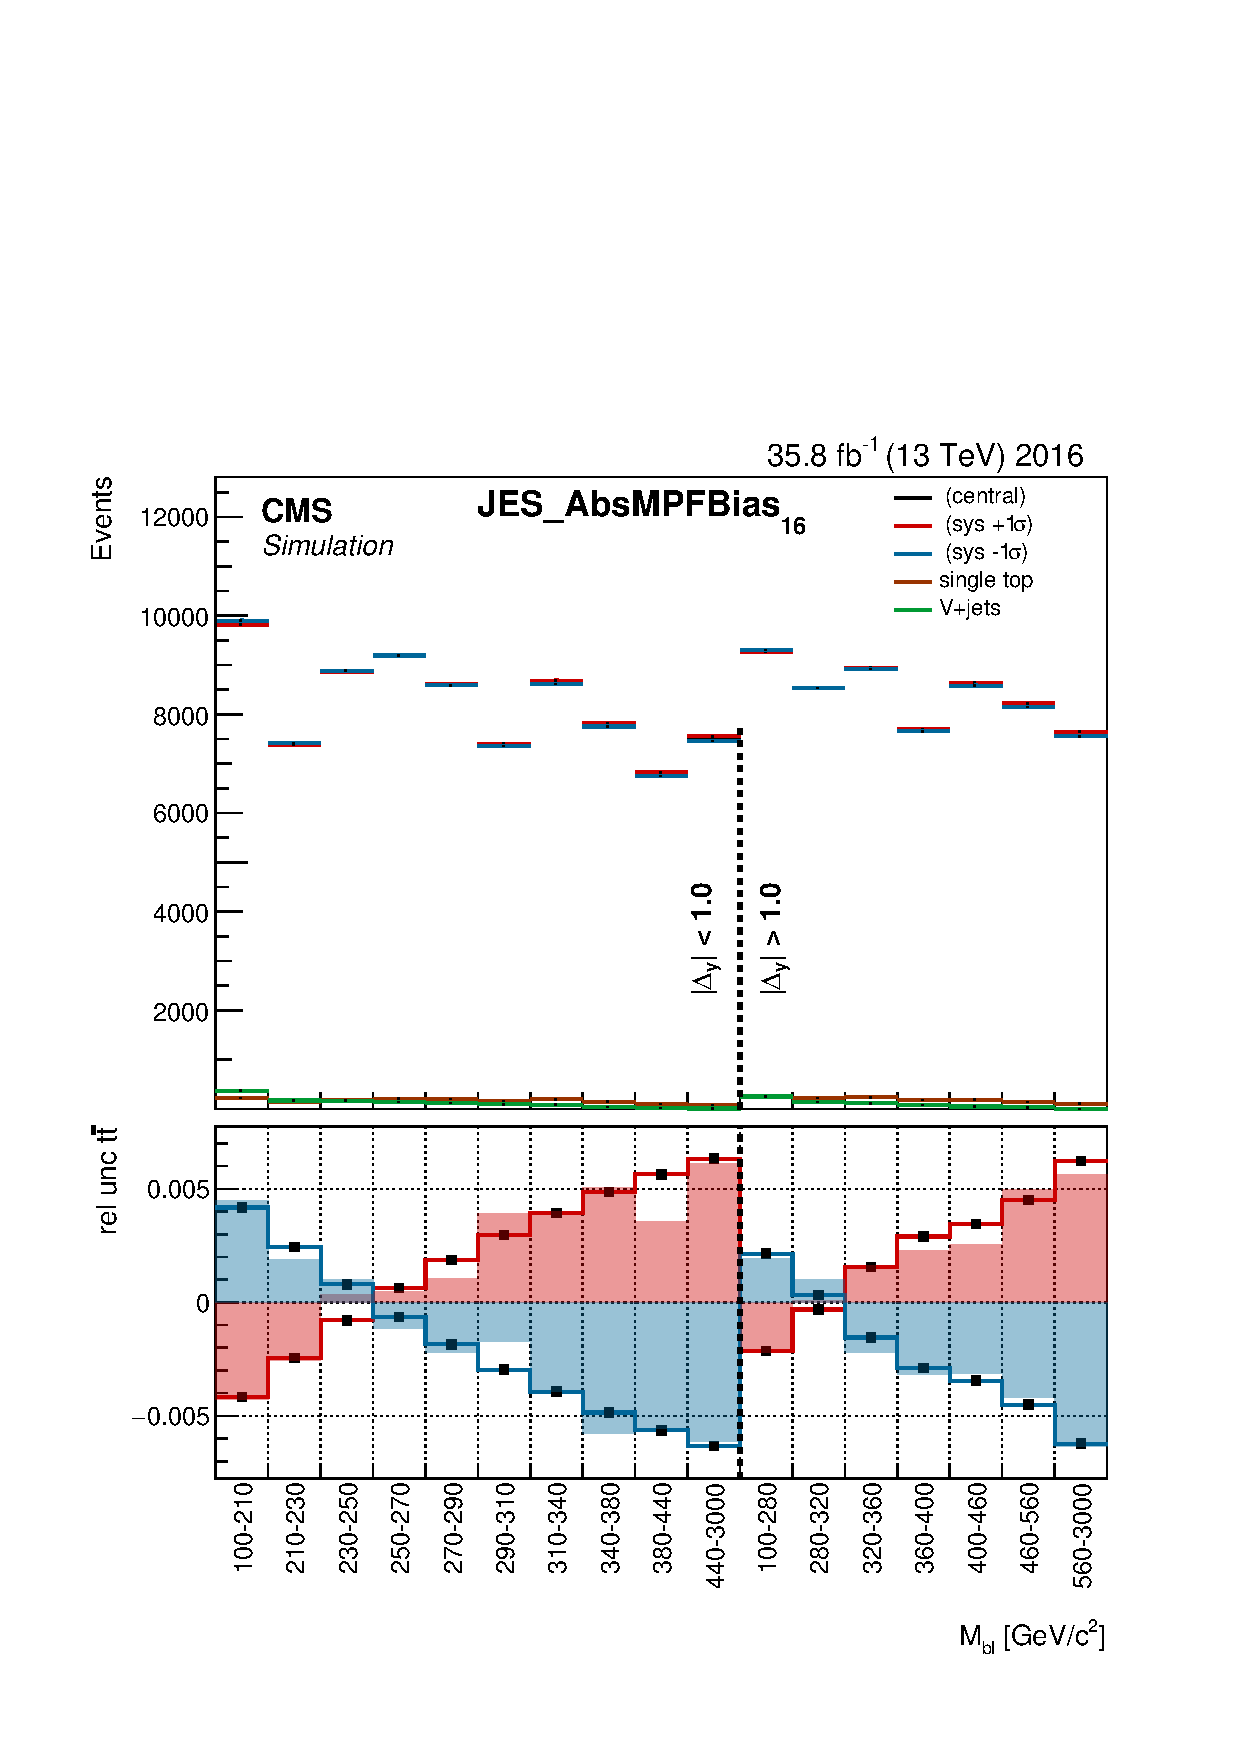
\includegraphics[width=.35\linewidth]{templates/JES_AbsoluteMPFBias_16}\hskip-.5cm
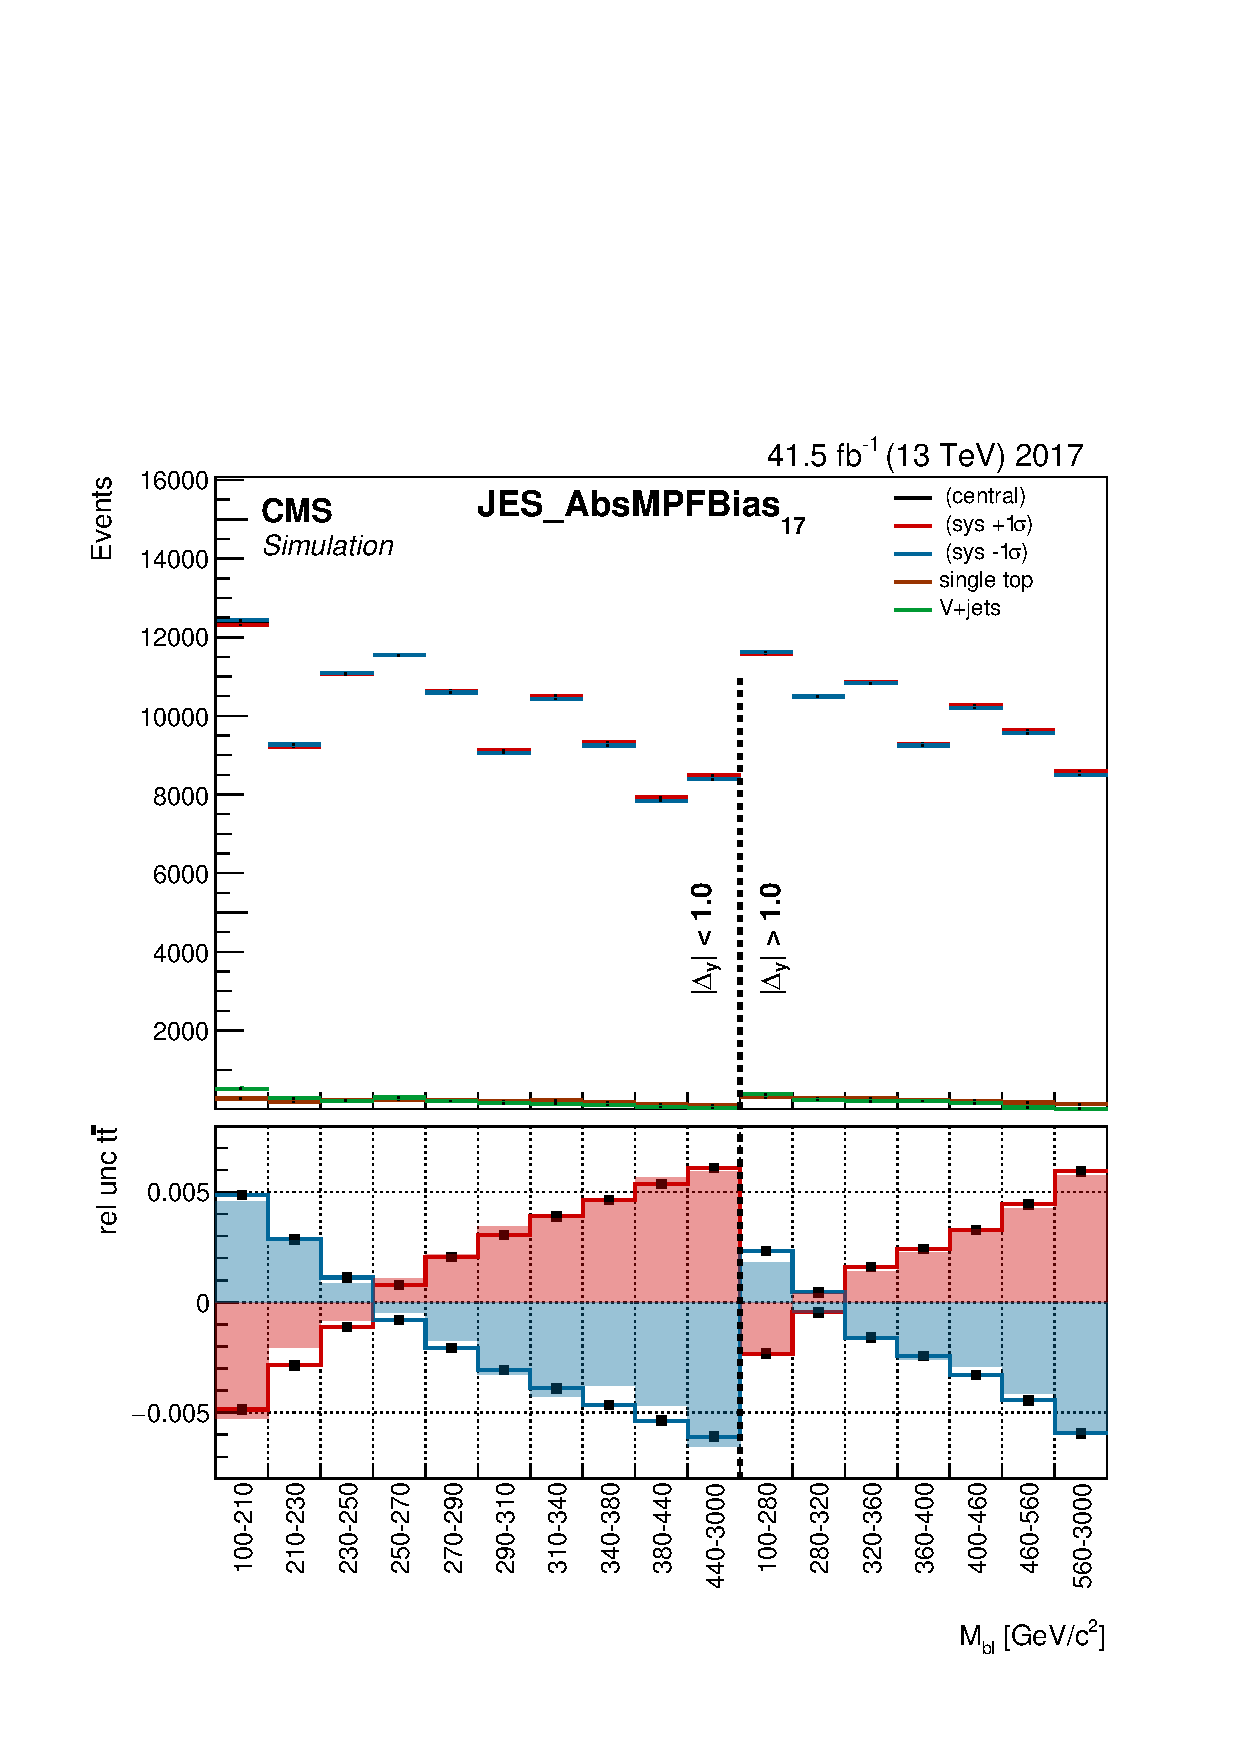
\includegraphics[width=.35\linewidth]{templates/JES_AbsoluteMPFBias_17}\hskip-.5cm
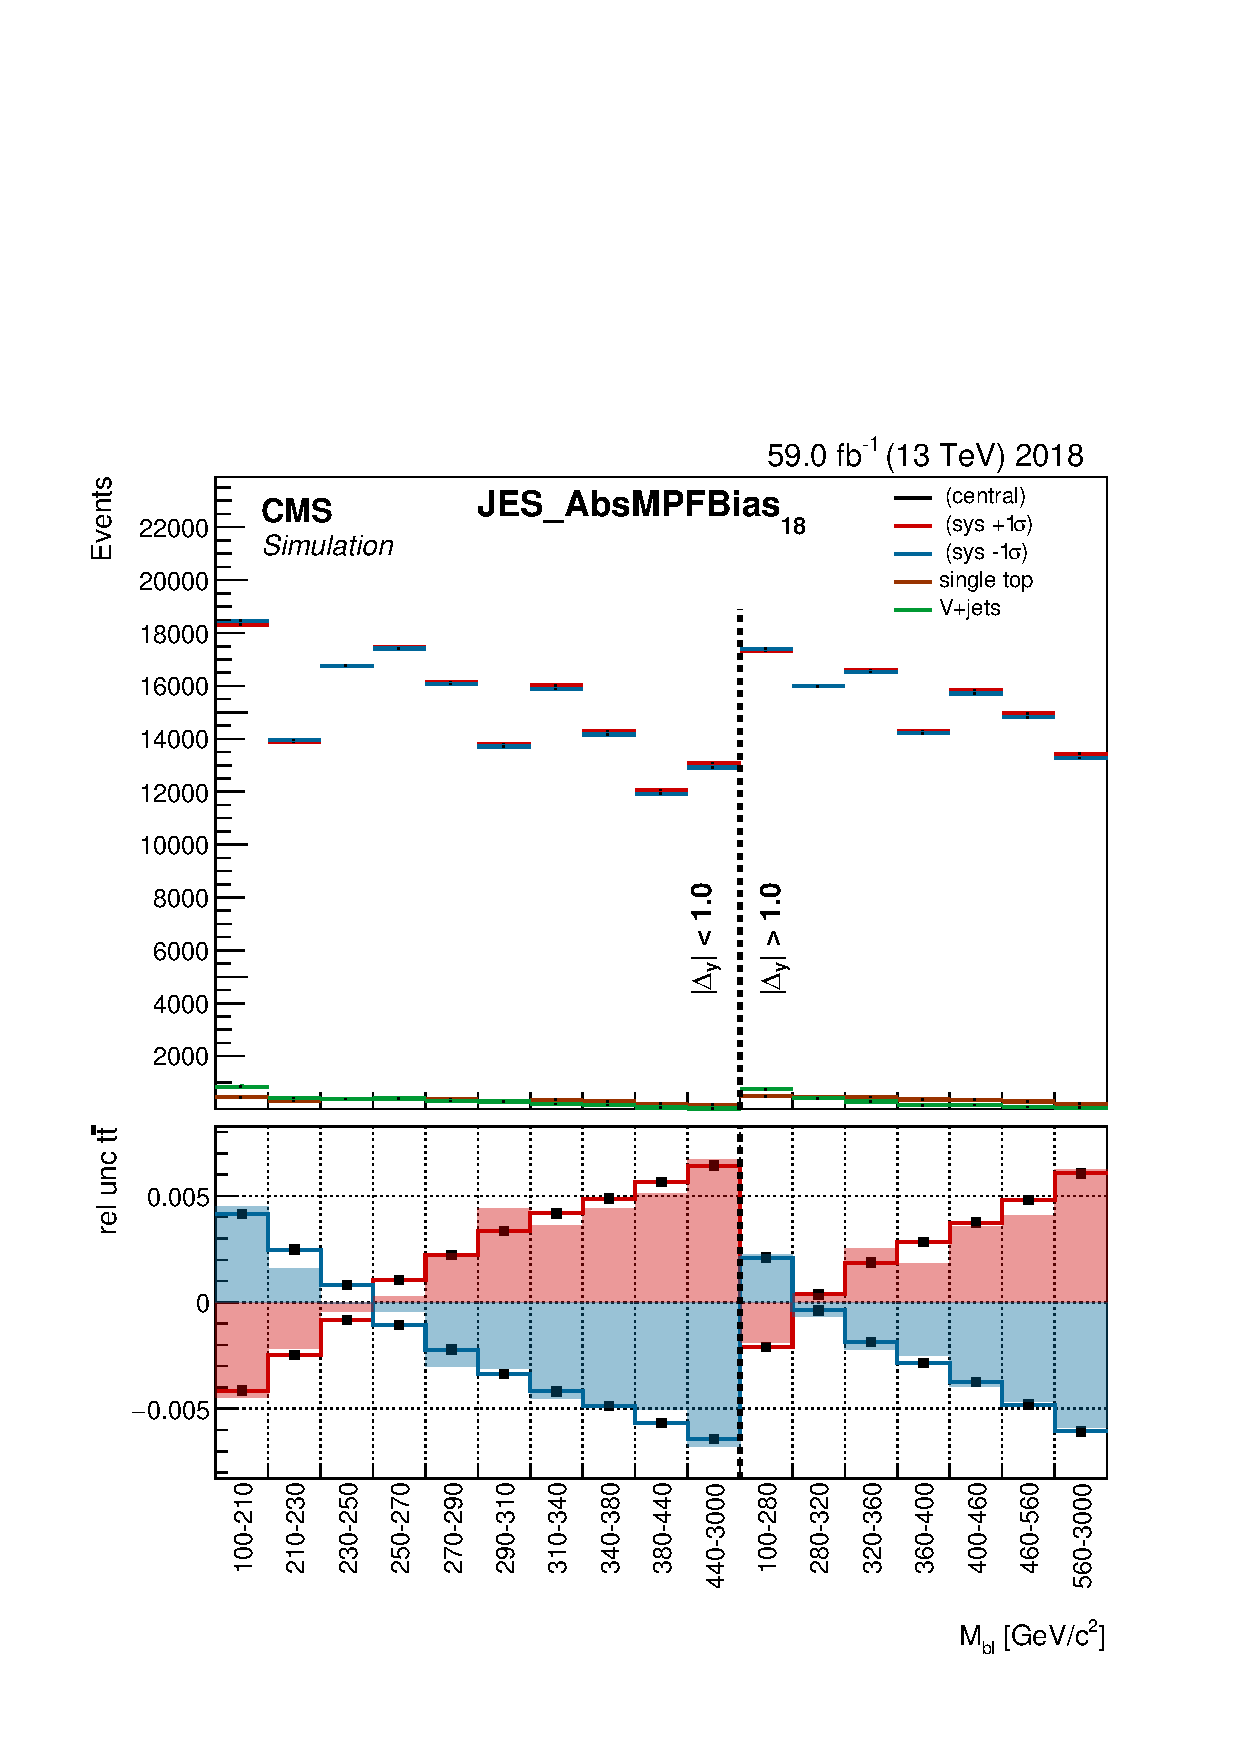
\includegraphics[width=.35\linewidth]{templates/JES_AbsoluteMPFBias_18}
\caption{JES\_AbsoluteMPFBias templates}
\label{fig:JES-AbsoluteMPFBias_template}
\end{figure}

\begin{figure} \centering
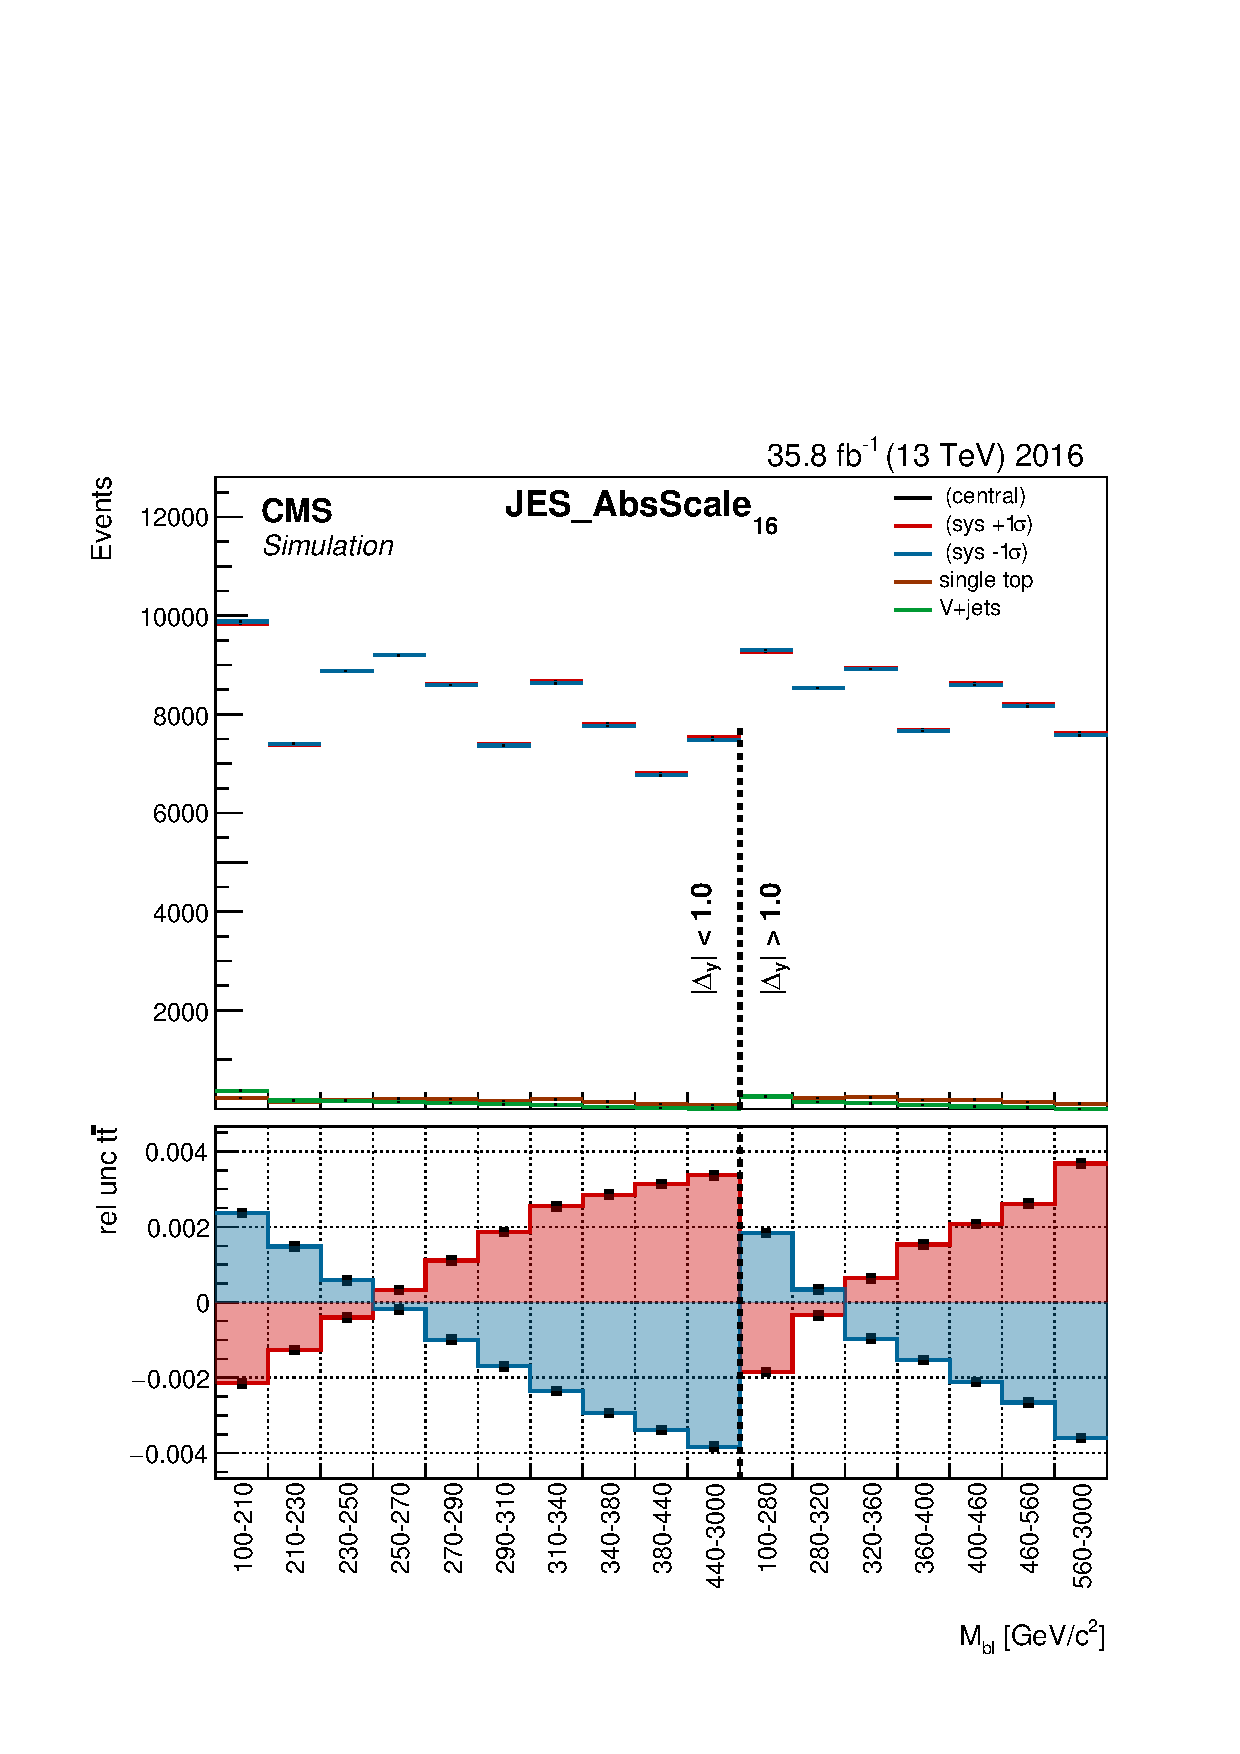
\includegraphics[width=.35\linewidth]{templates/JES_AbsoluteScale_16}\hskip-.5cm
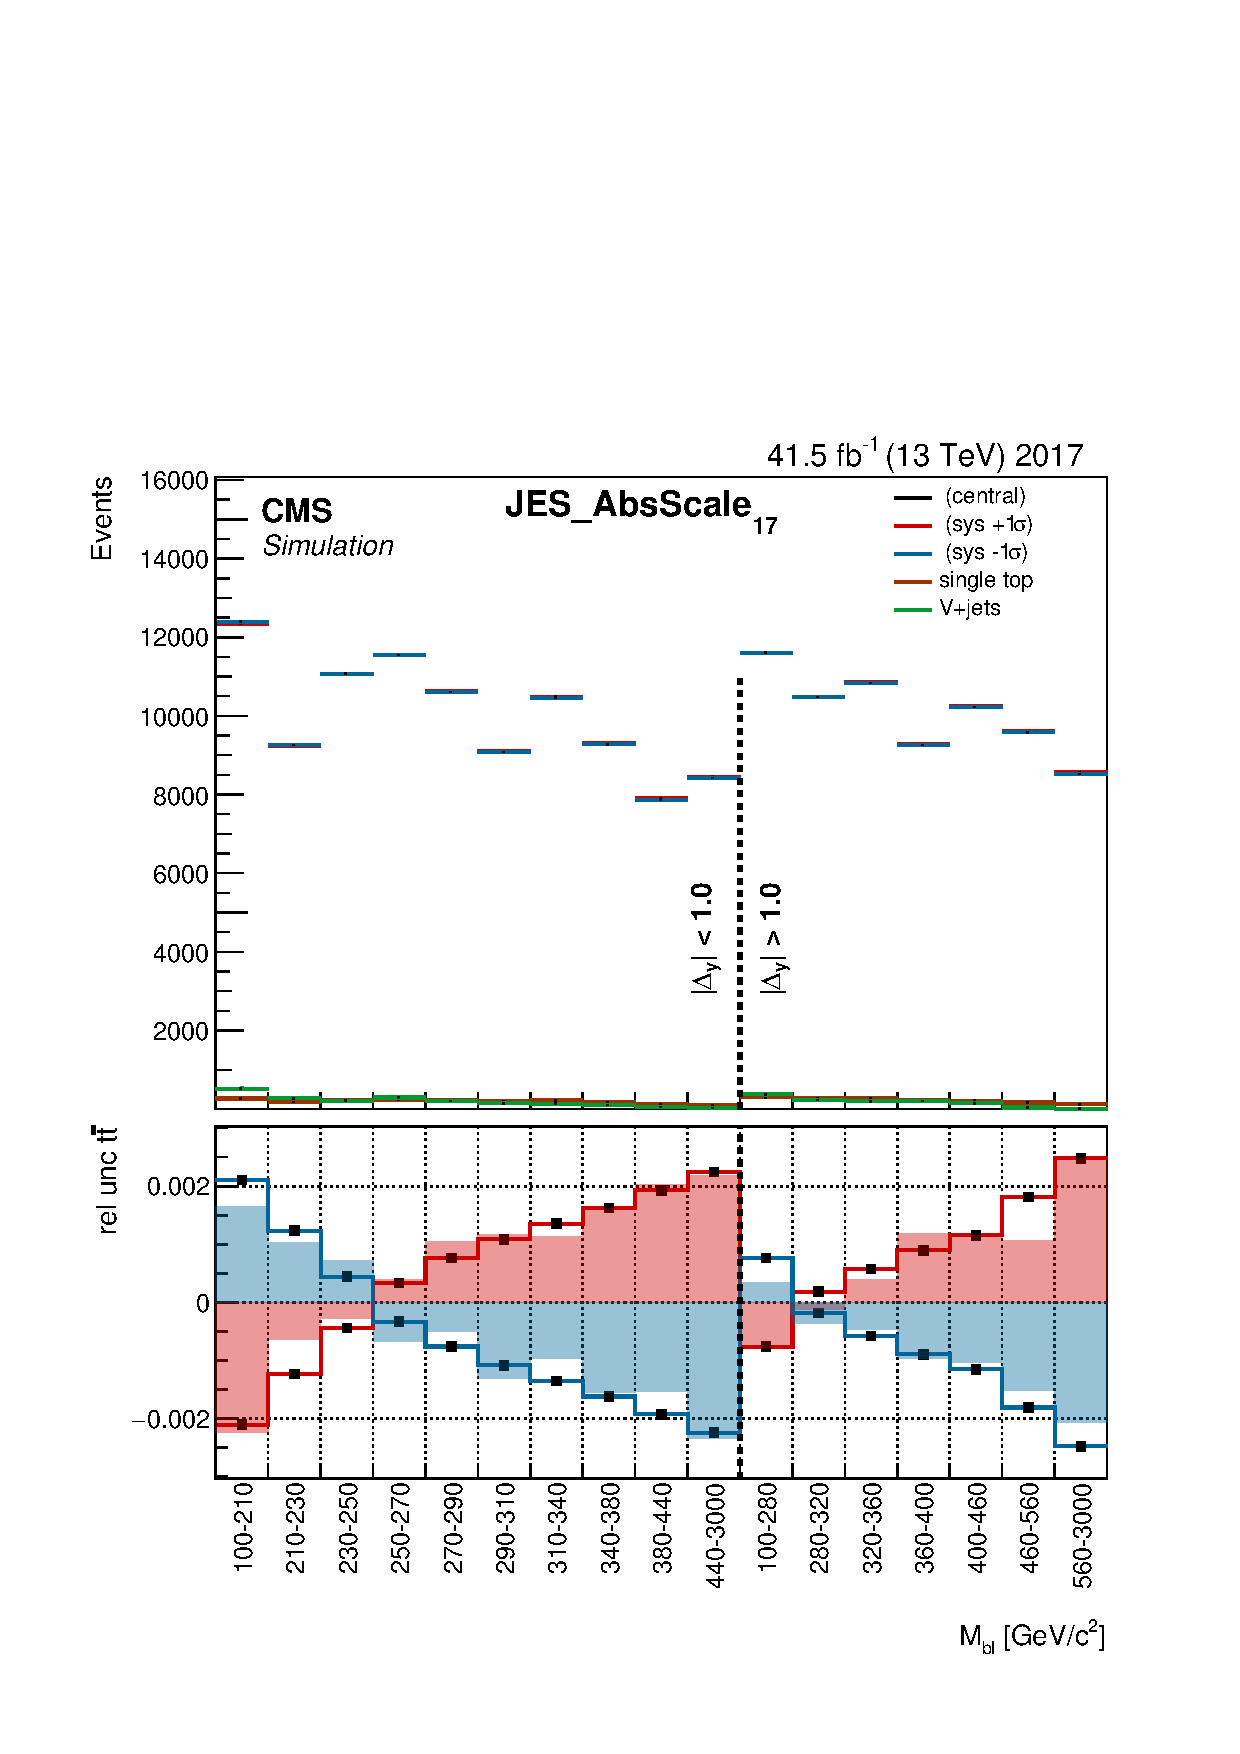
\includegraphics[width=.35\linewidth]{templates/JES_AbsoluteScale_17}\hskip-.5cm
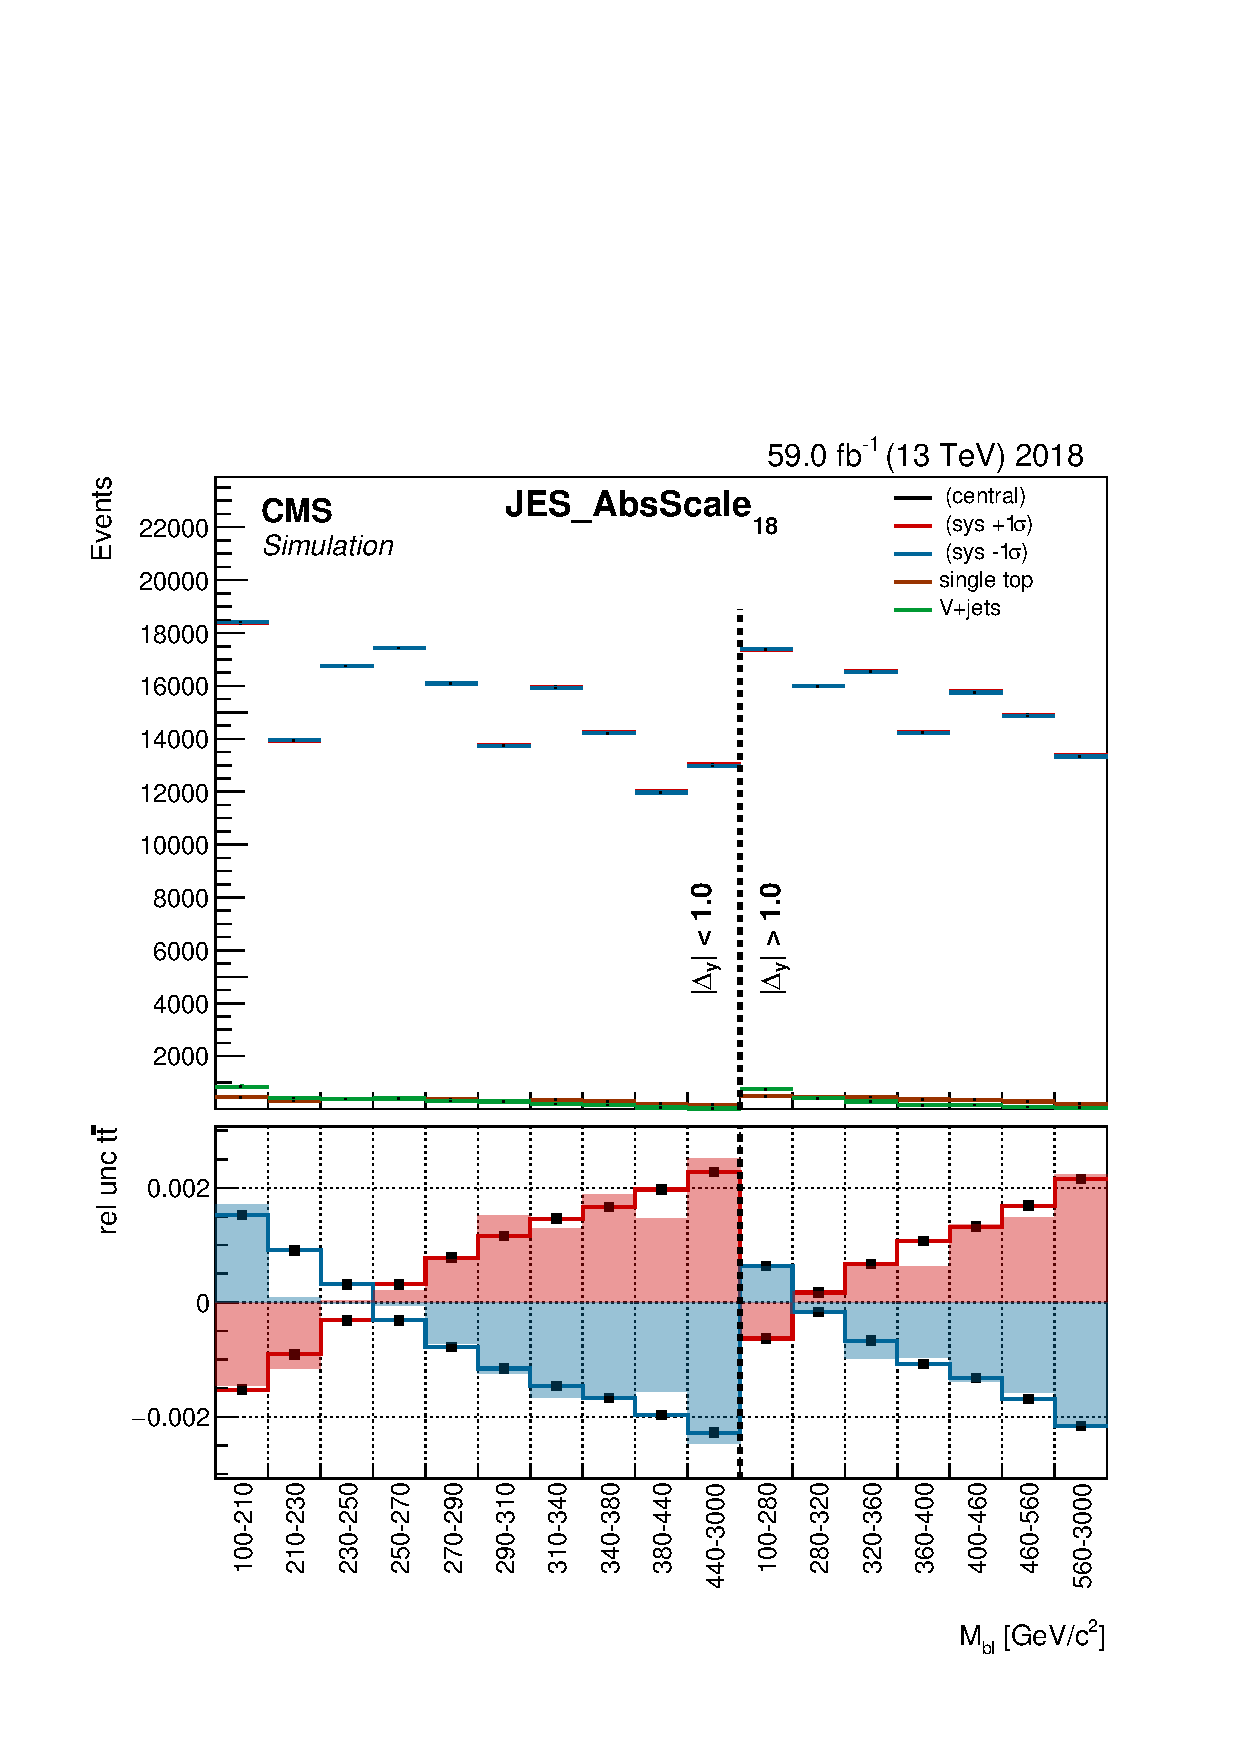
\includegraphics[width=.35\linewidth]{templates/JES_AbsoluteScale_18}
\caption{JES\_AbsoluteScale templates}
\label{fig:JES-AbsoluteScale_template}
\end{figure}

\begin{figure} \centering
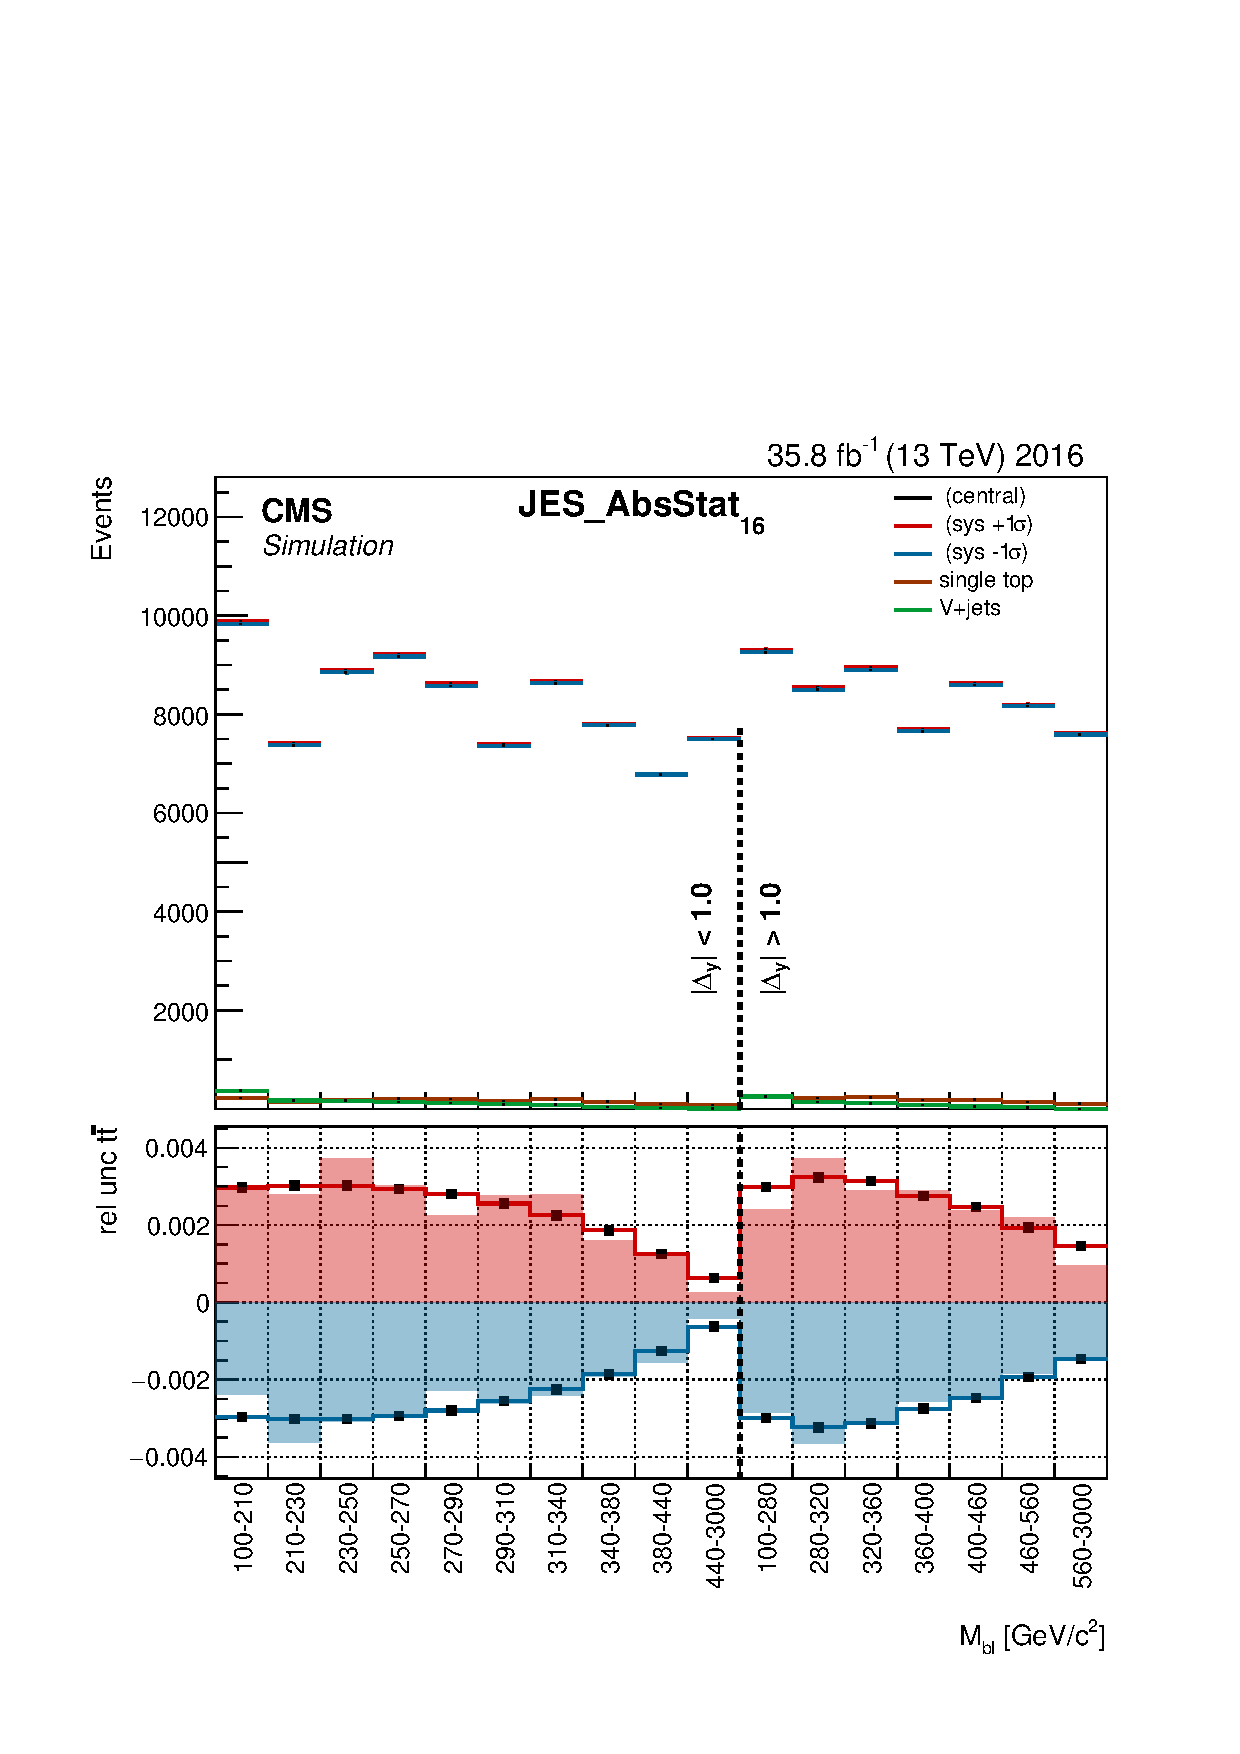
\includegraphics[width=.35\linewidth]{templates/JES_AbsoluteStat_16}\hskip-.5cm
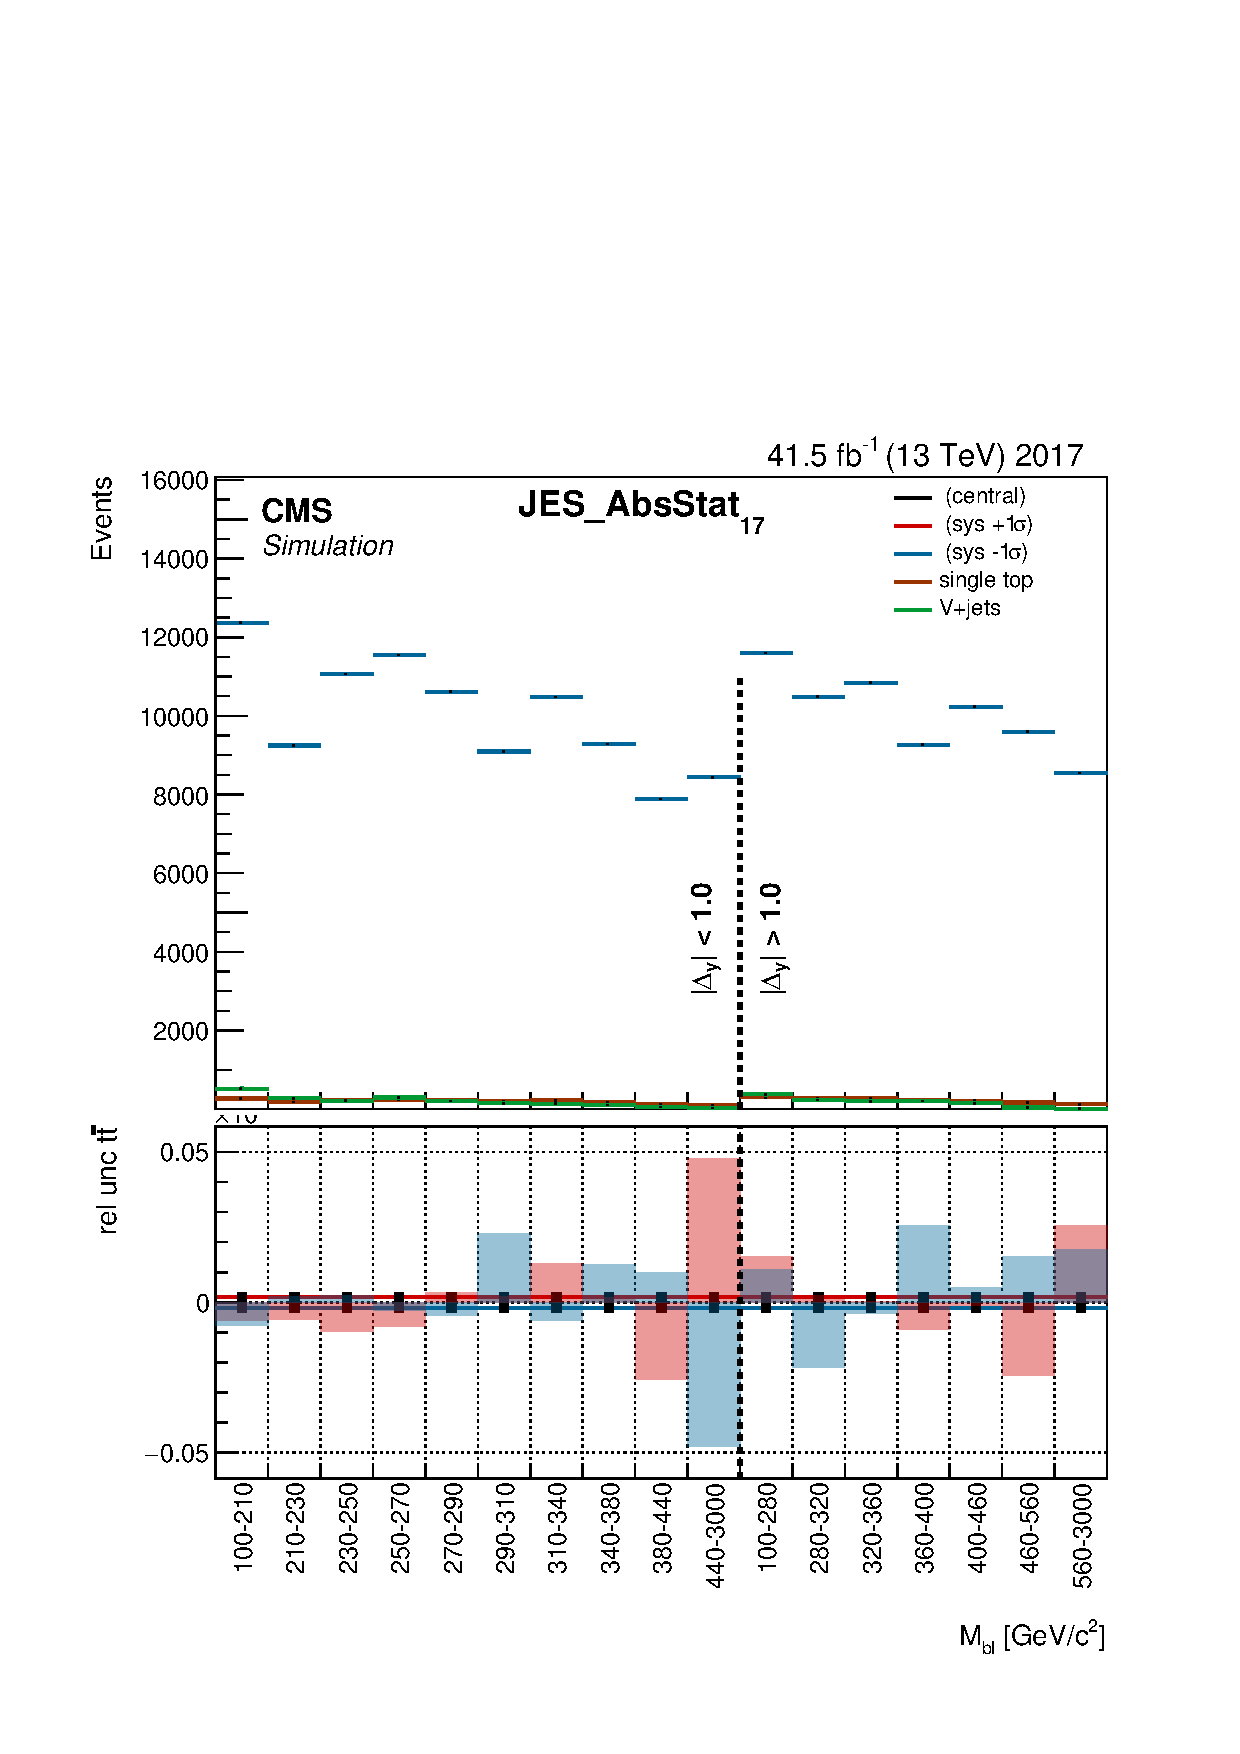
\includegraphics[width=.35\linewidth]{templates/JES_AbsoluteStat_17}\hskip-.5cm
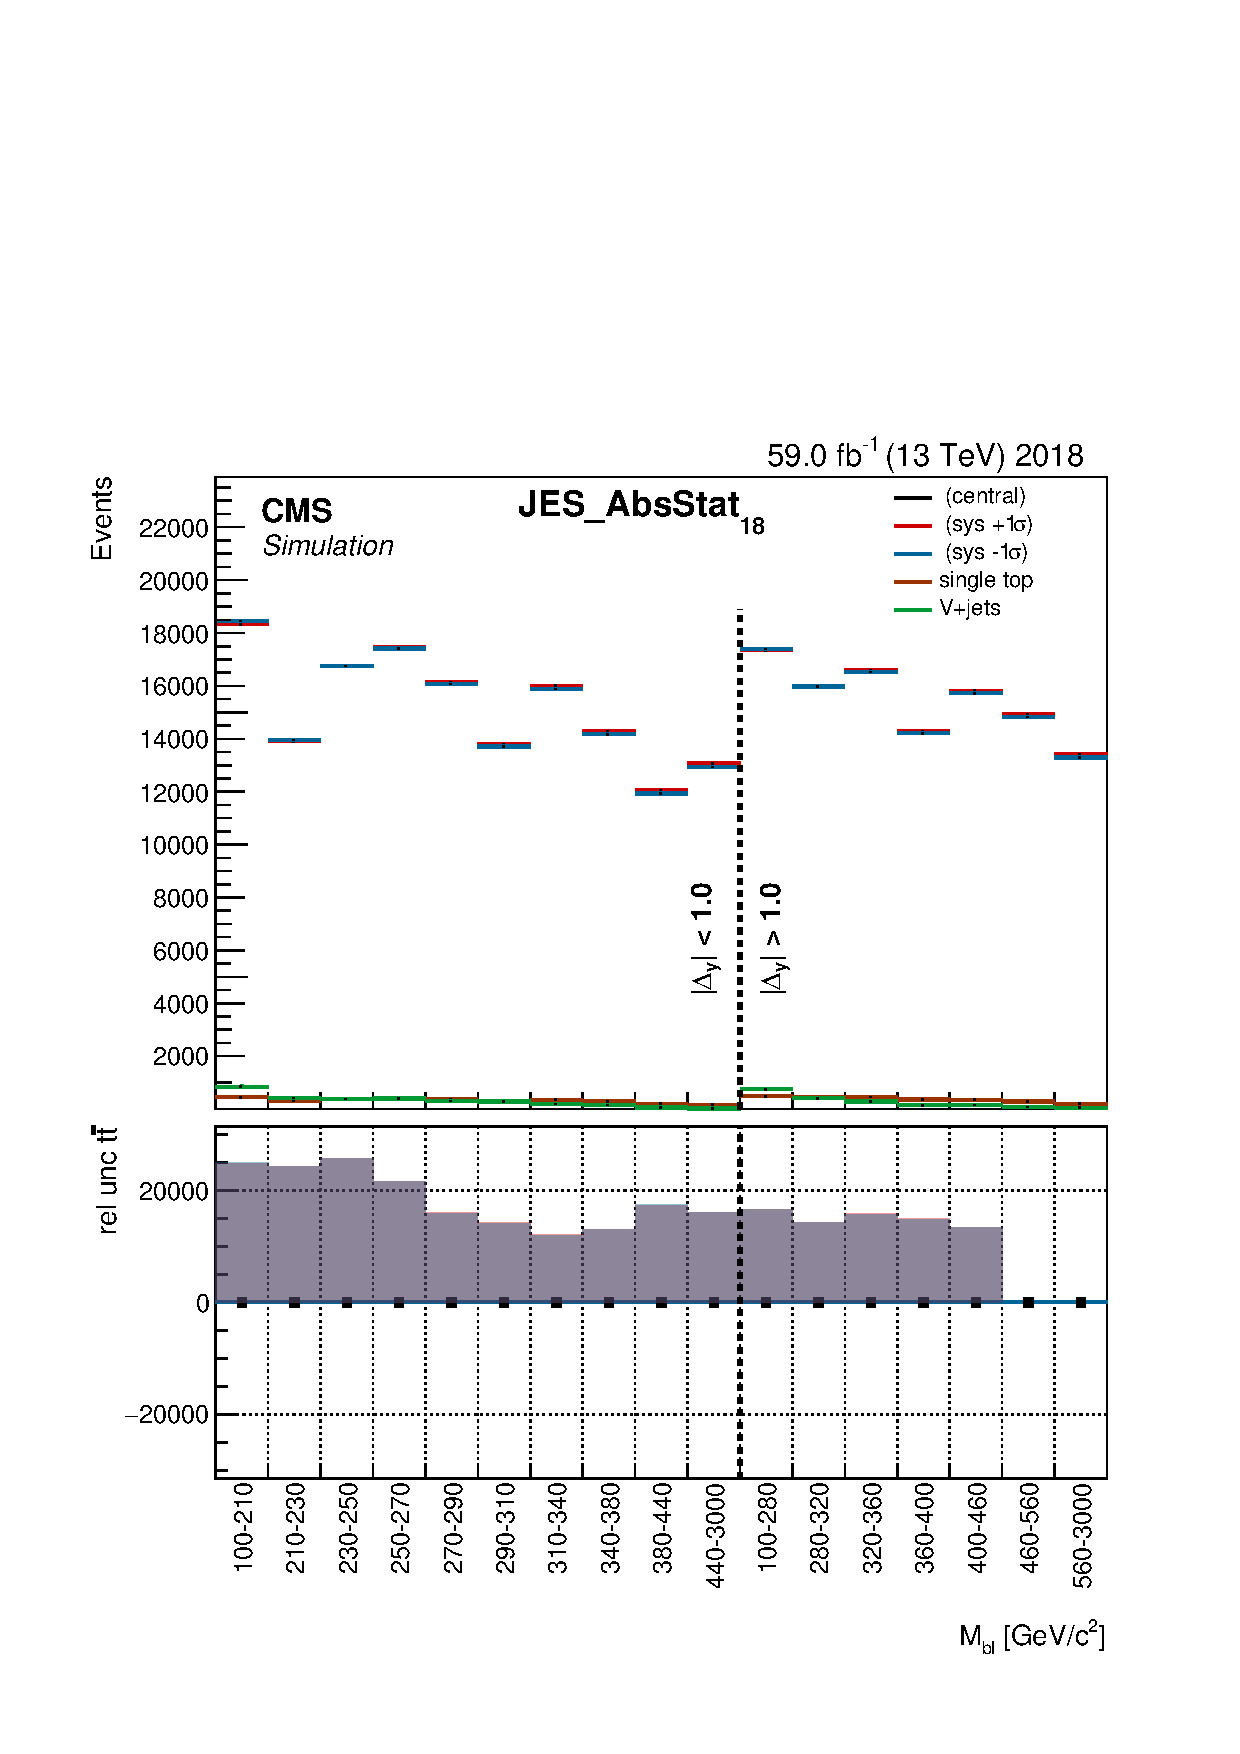
\includegraphics[width=.35\linewidth]{templates/JES_AbsoluteStat_18}
\caption{JES\_AbsoluteStat templates}
\label{fig:JES-AbsoluteStat_template}
\end{figure}

\begin{figure} \centering
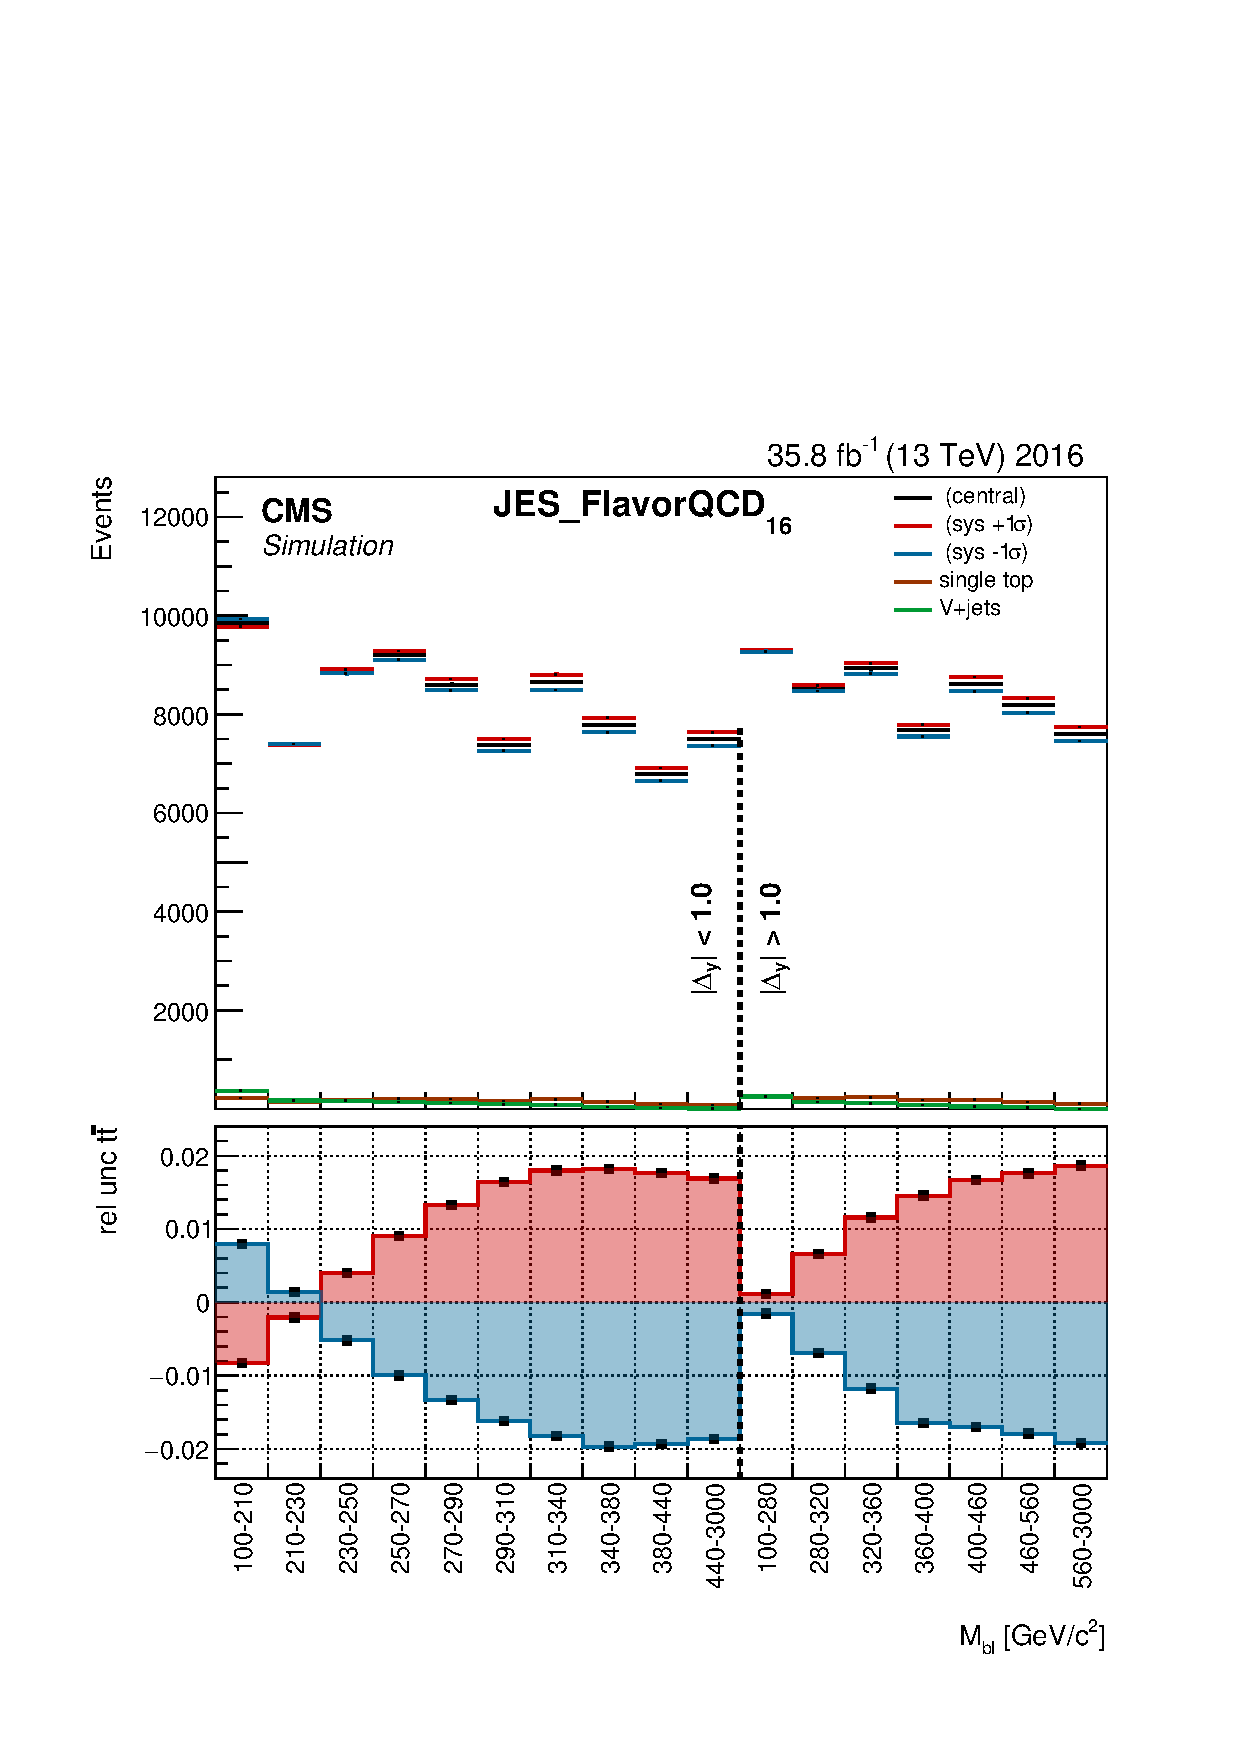
\includegraphics[width=.35\linewidth]{templates/JES_FlavorQCD_16}\hskip-.5cm
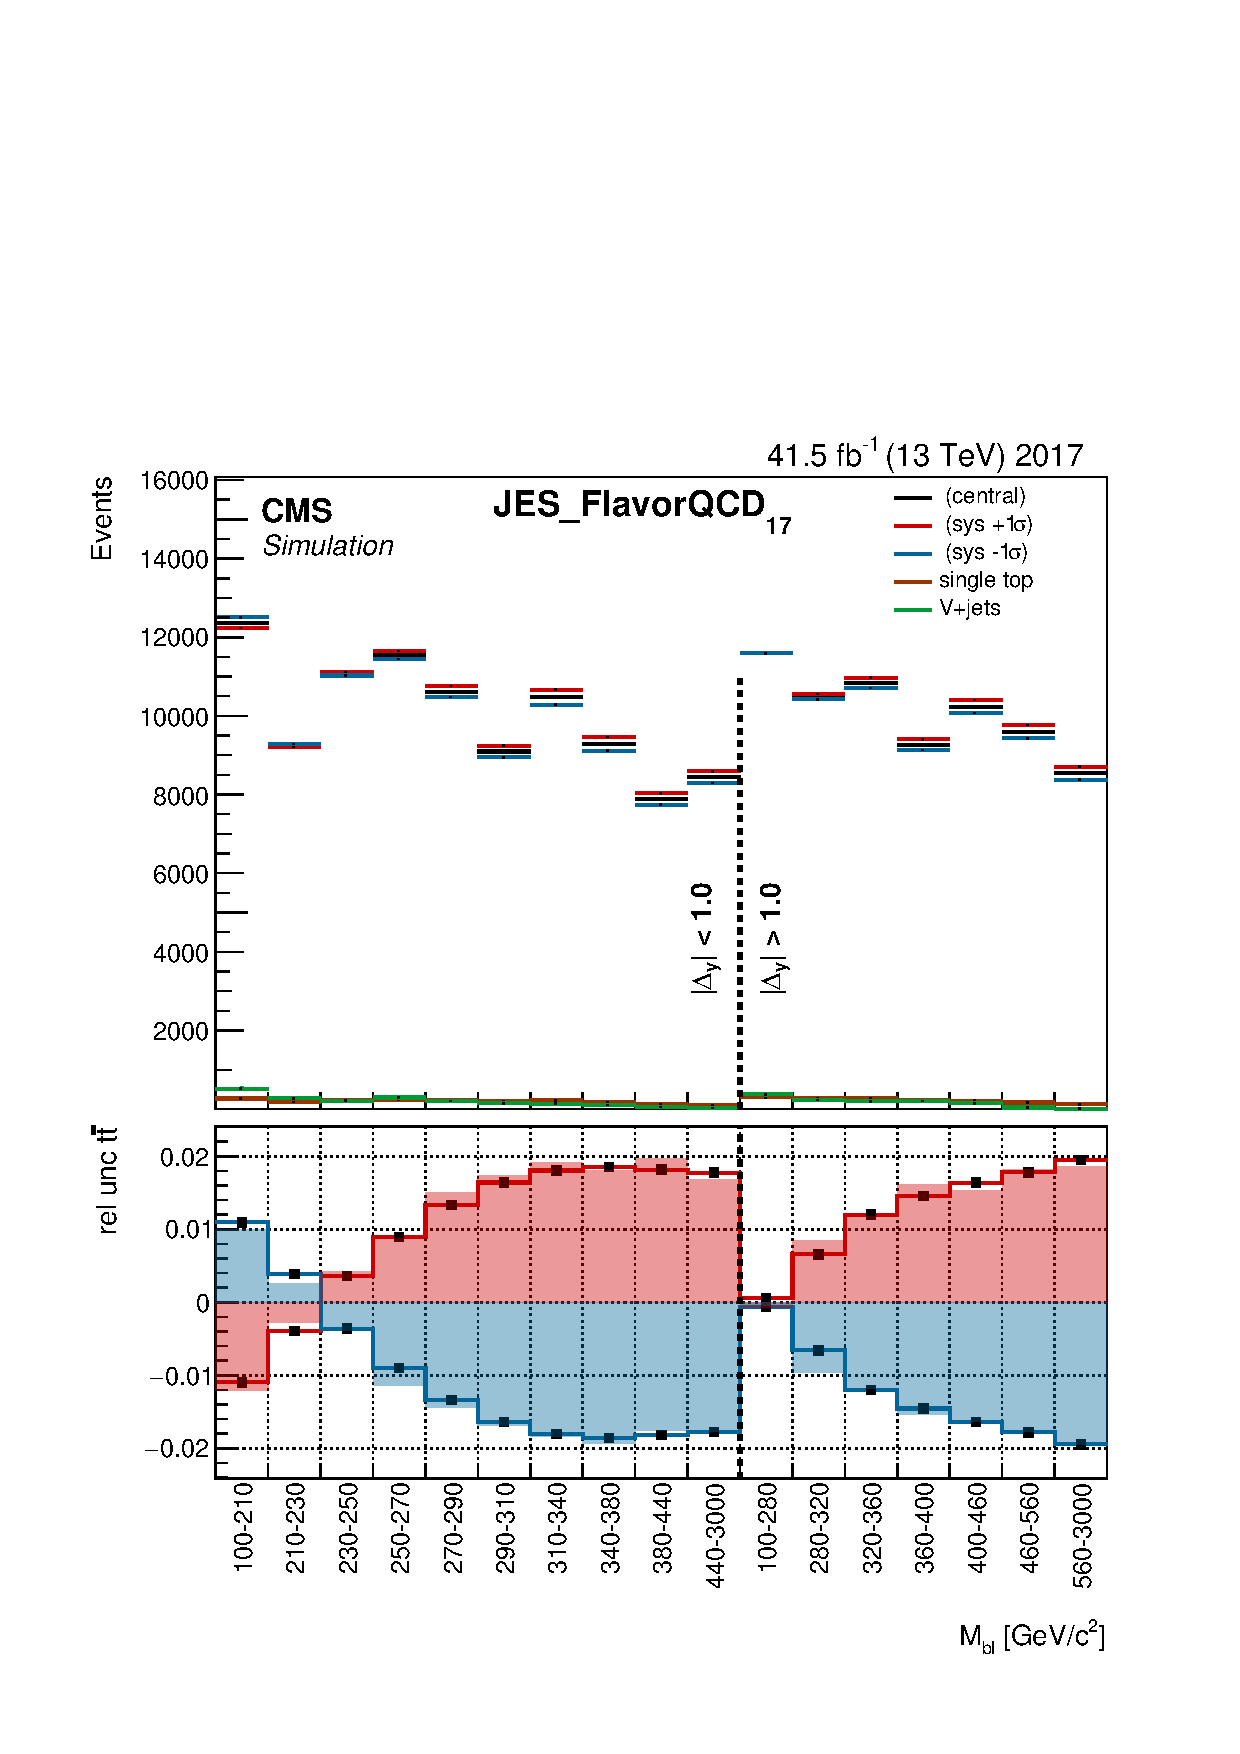
\includegraphics[width=.35\linewidth]{templates/JES_FlavorQCD_17}\hskip-.5cm
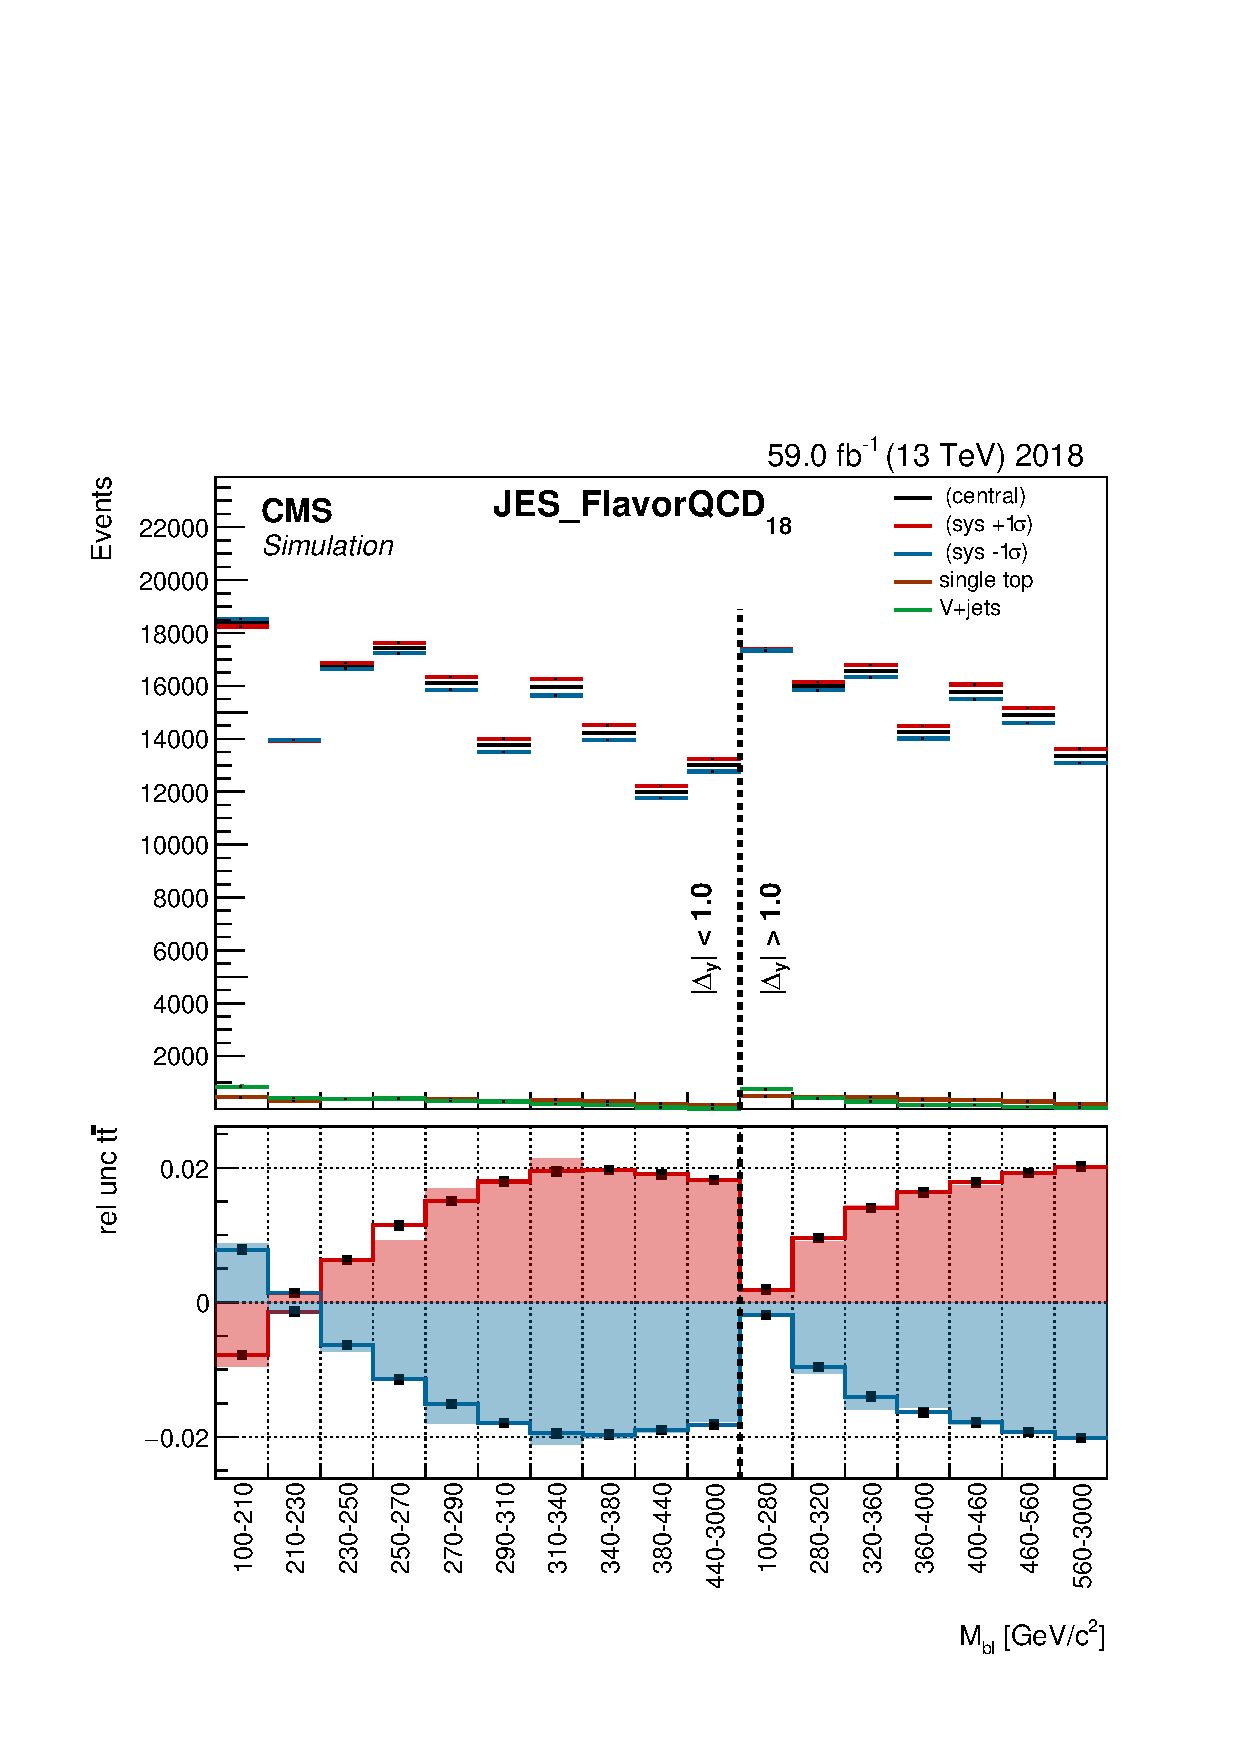
\includegraphics[width=.35\linewidth]{templates/JES_FlavorQCD_18}
\caption{JES\_FlavorQCD templates}
\label{fig:JES-FlavorQCD_template}
\end{figure}

\begin{figure} \centering
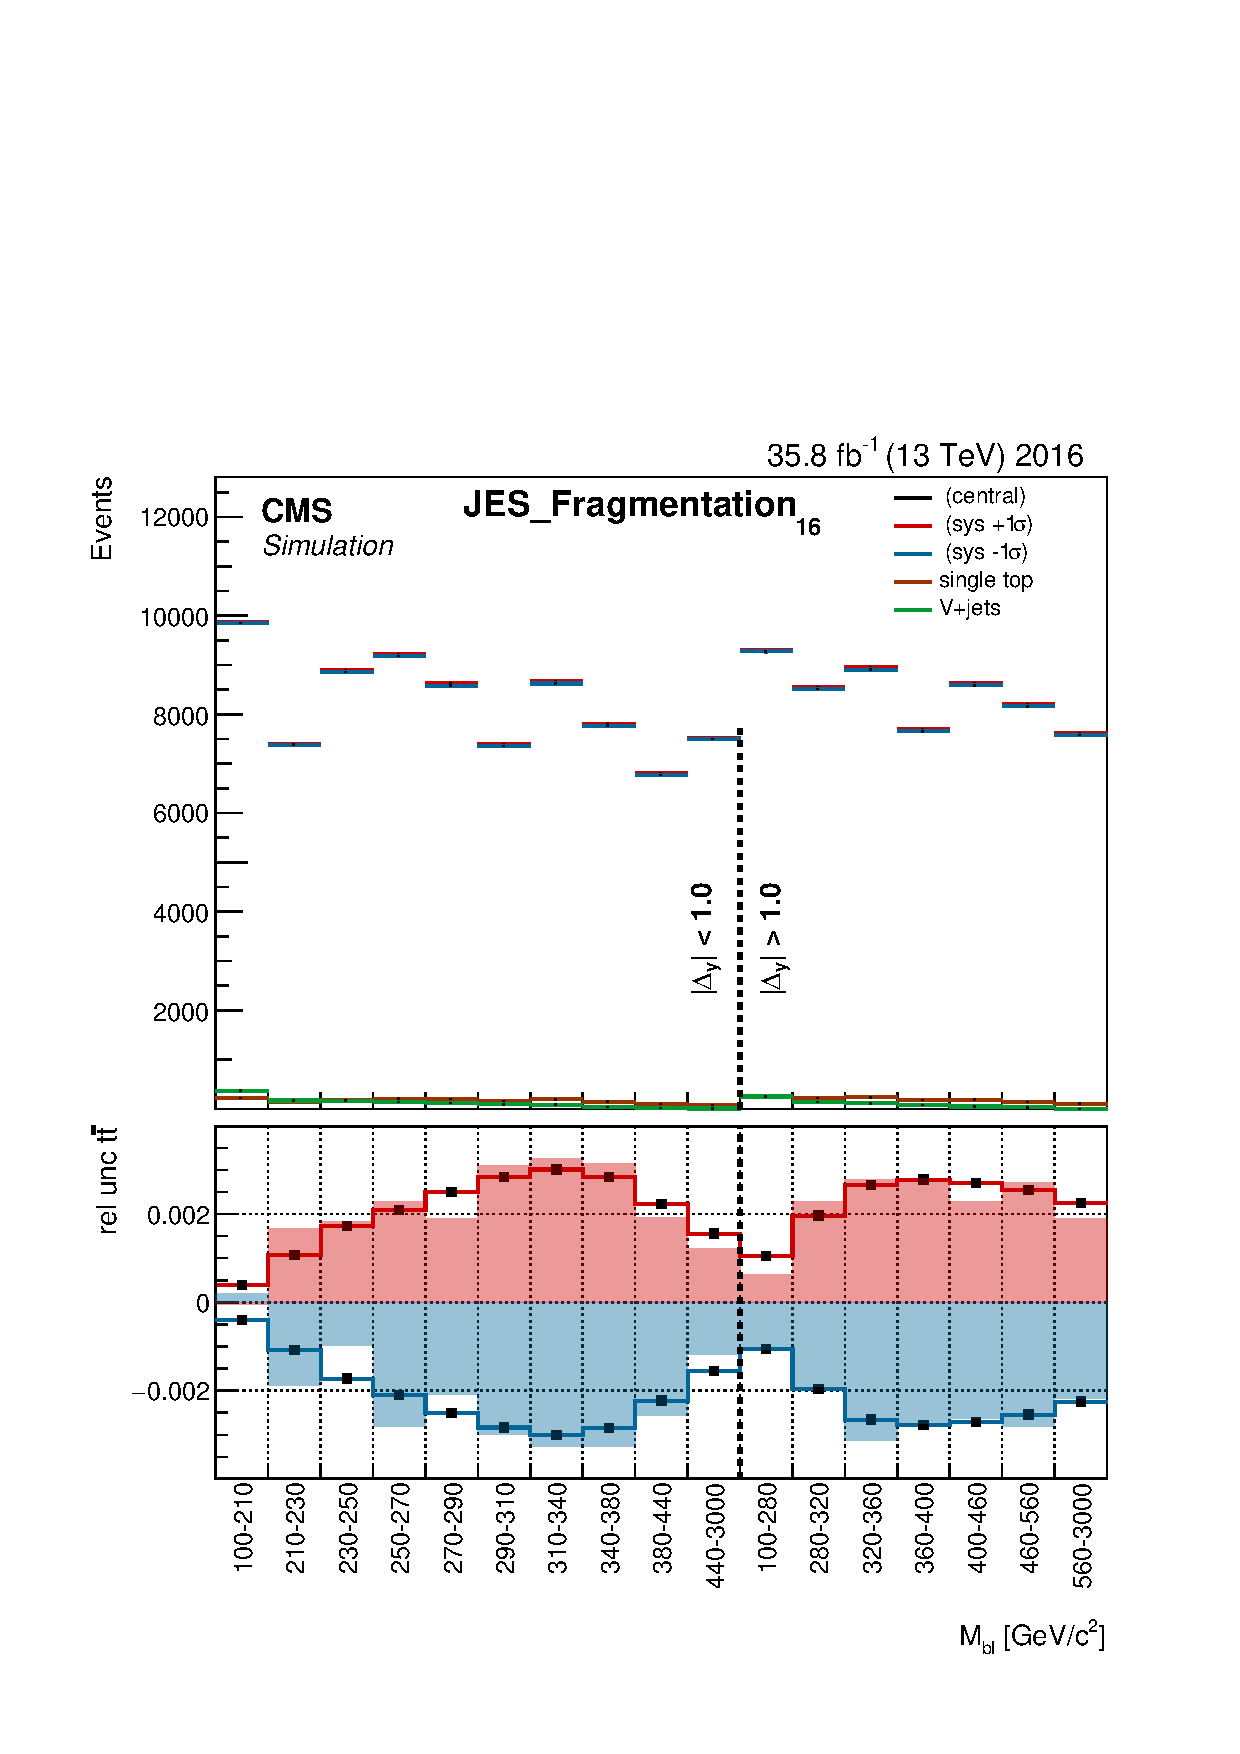
\includegraphics[width=.35\linewidth]{templates/JES_Fragmentation_16}\hskip-.5cm
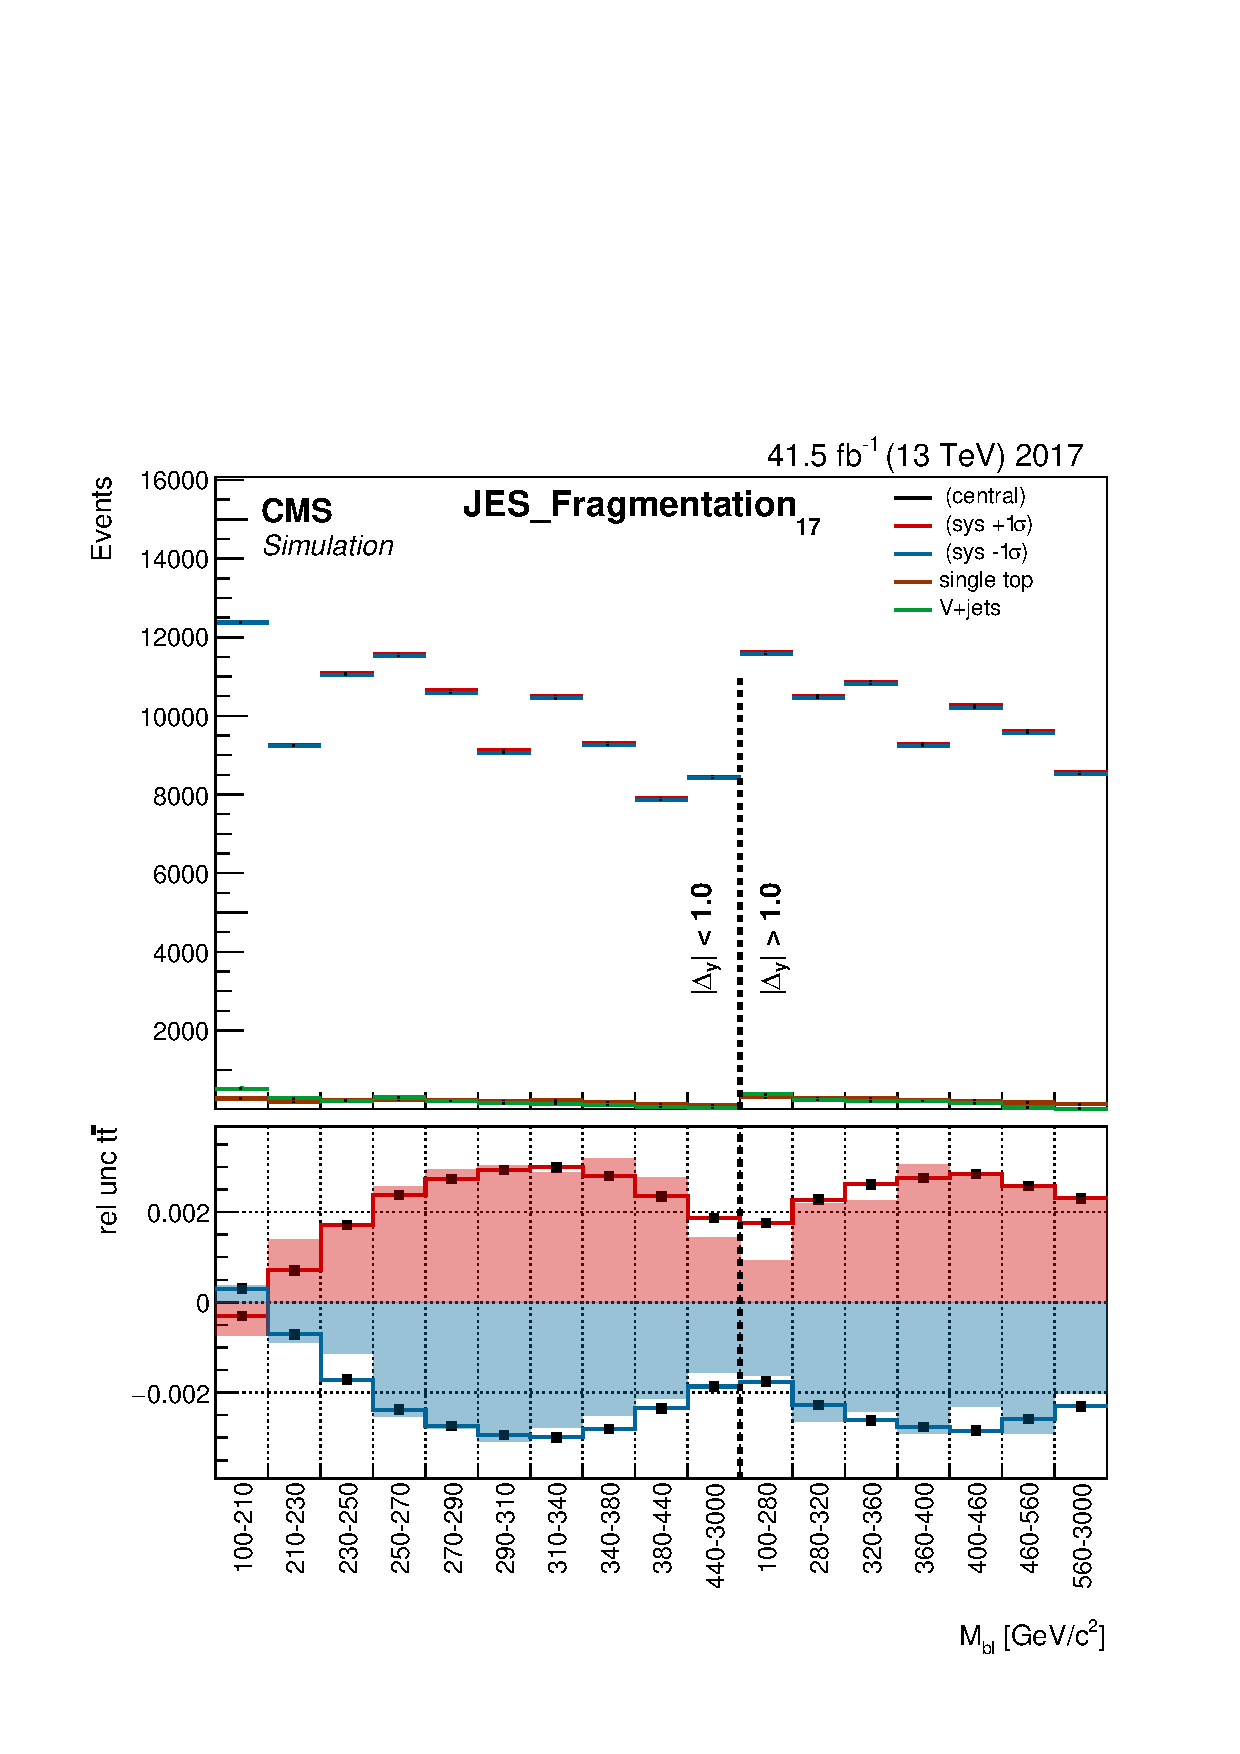
\includegraphics[width=.35\linewidth]{templates/JES_Fragmentation_17}\hskip-.5cm
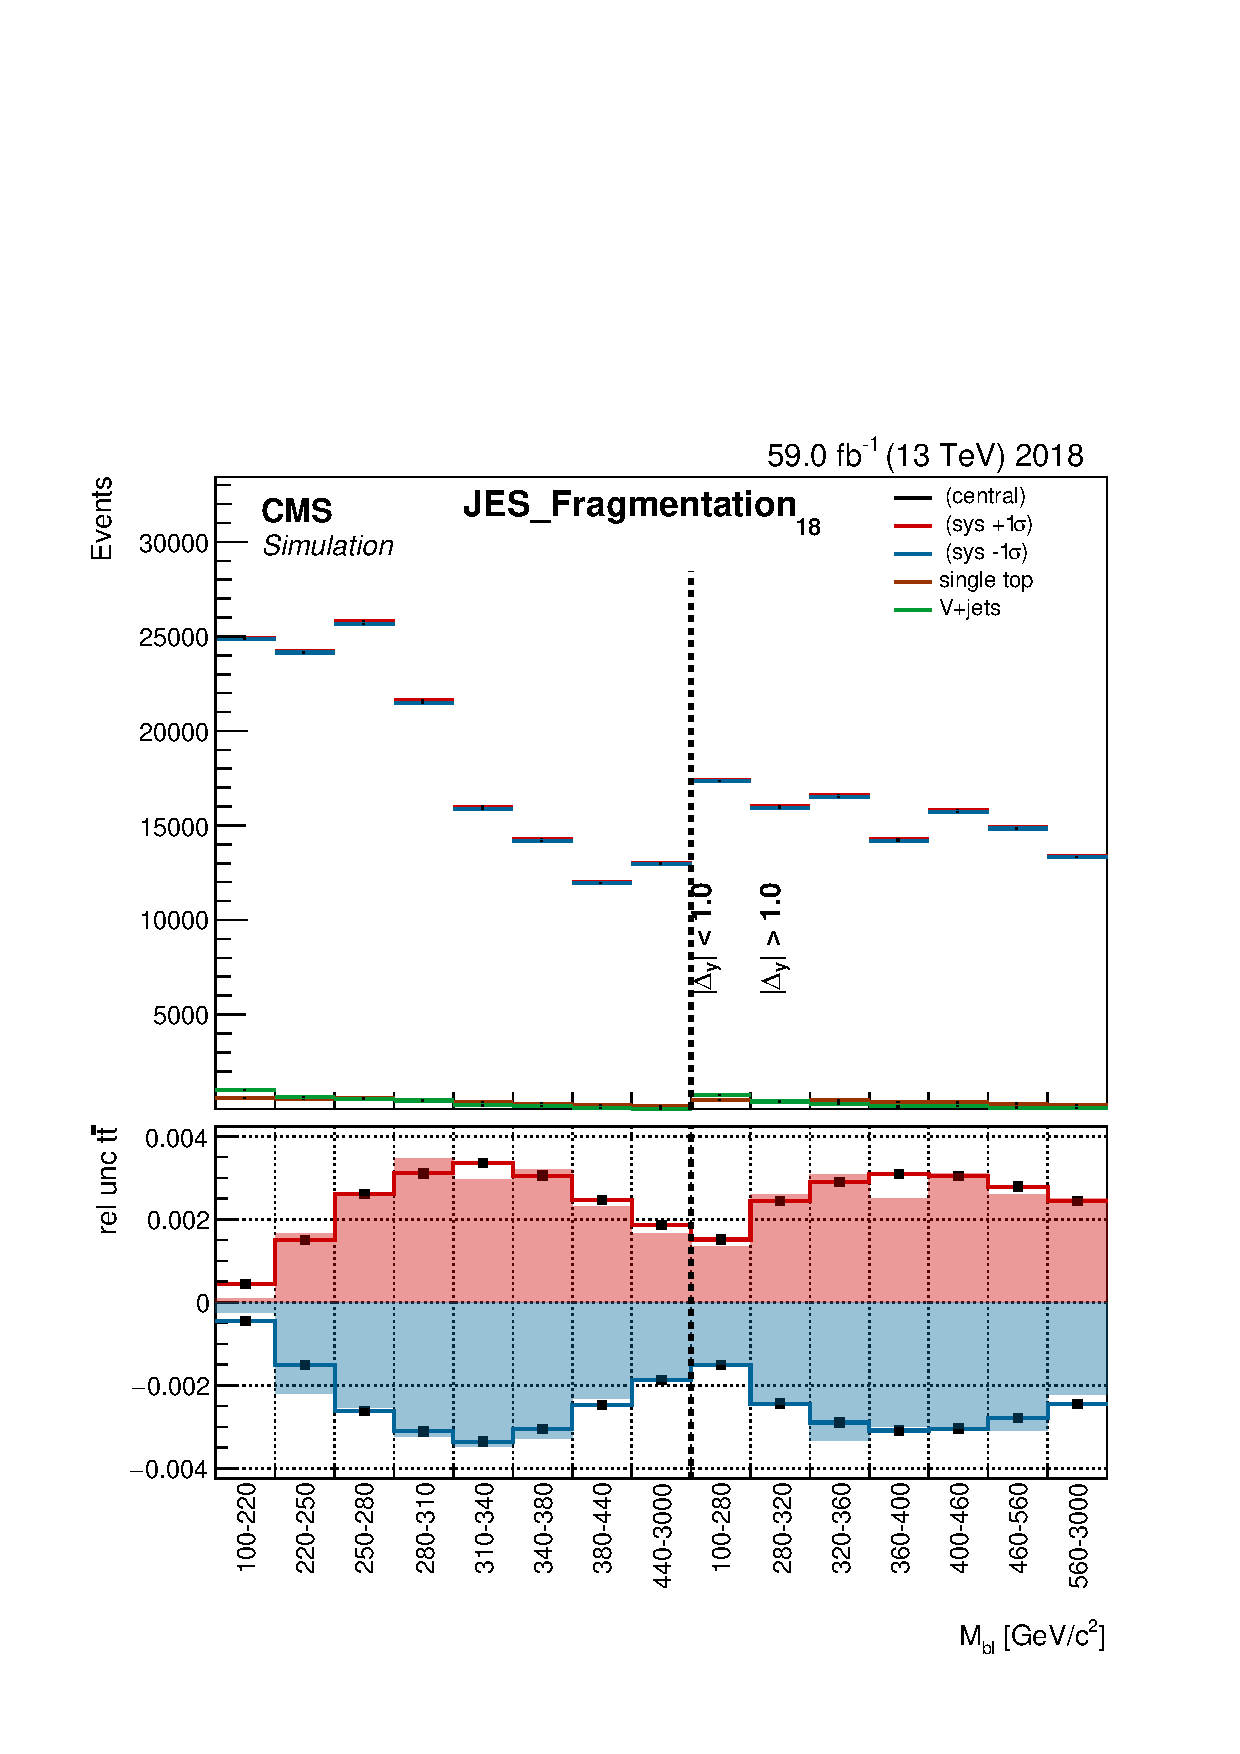
\includegraphics[width=.35\linewidth]{templates/JES_Fragmentation_18}
\caption{JES\_Fragmentation templates}
\label{fig:JES-Fragmentation_template}
\end{figure}

\begin{figure} \centering
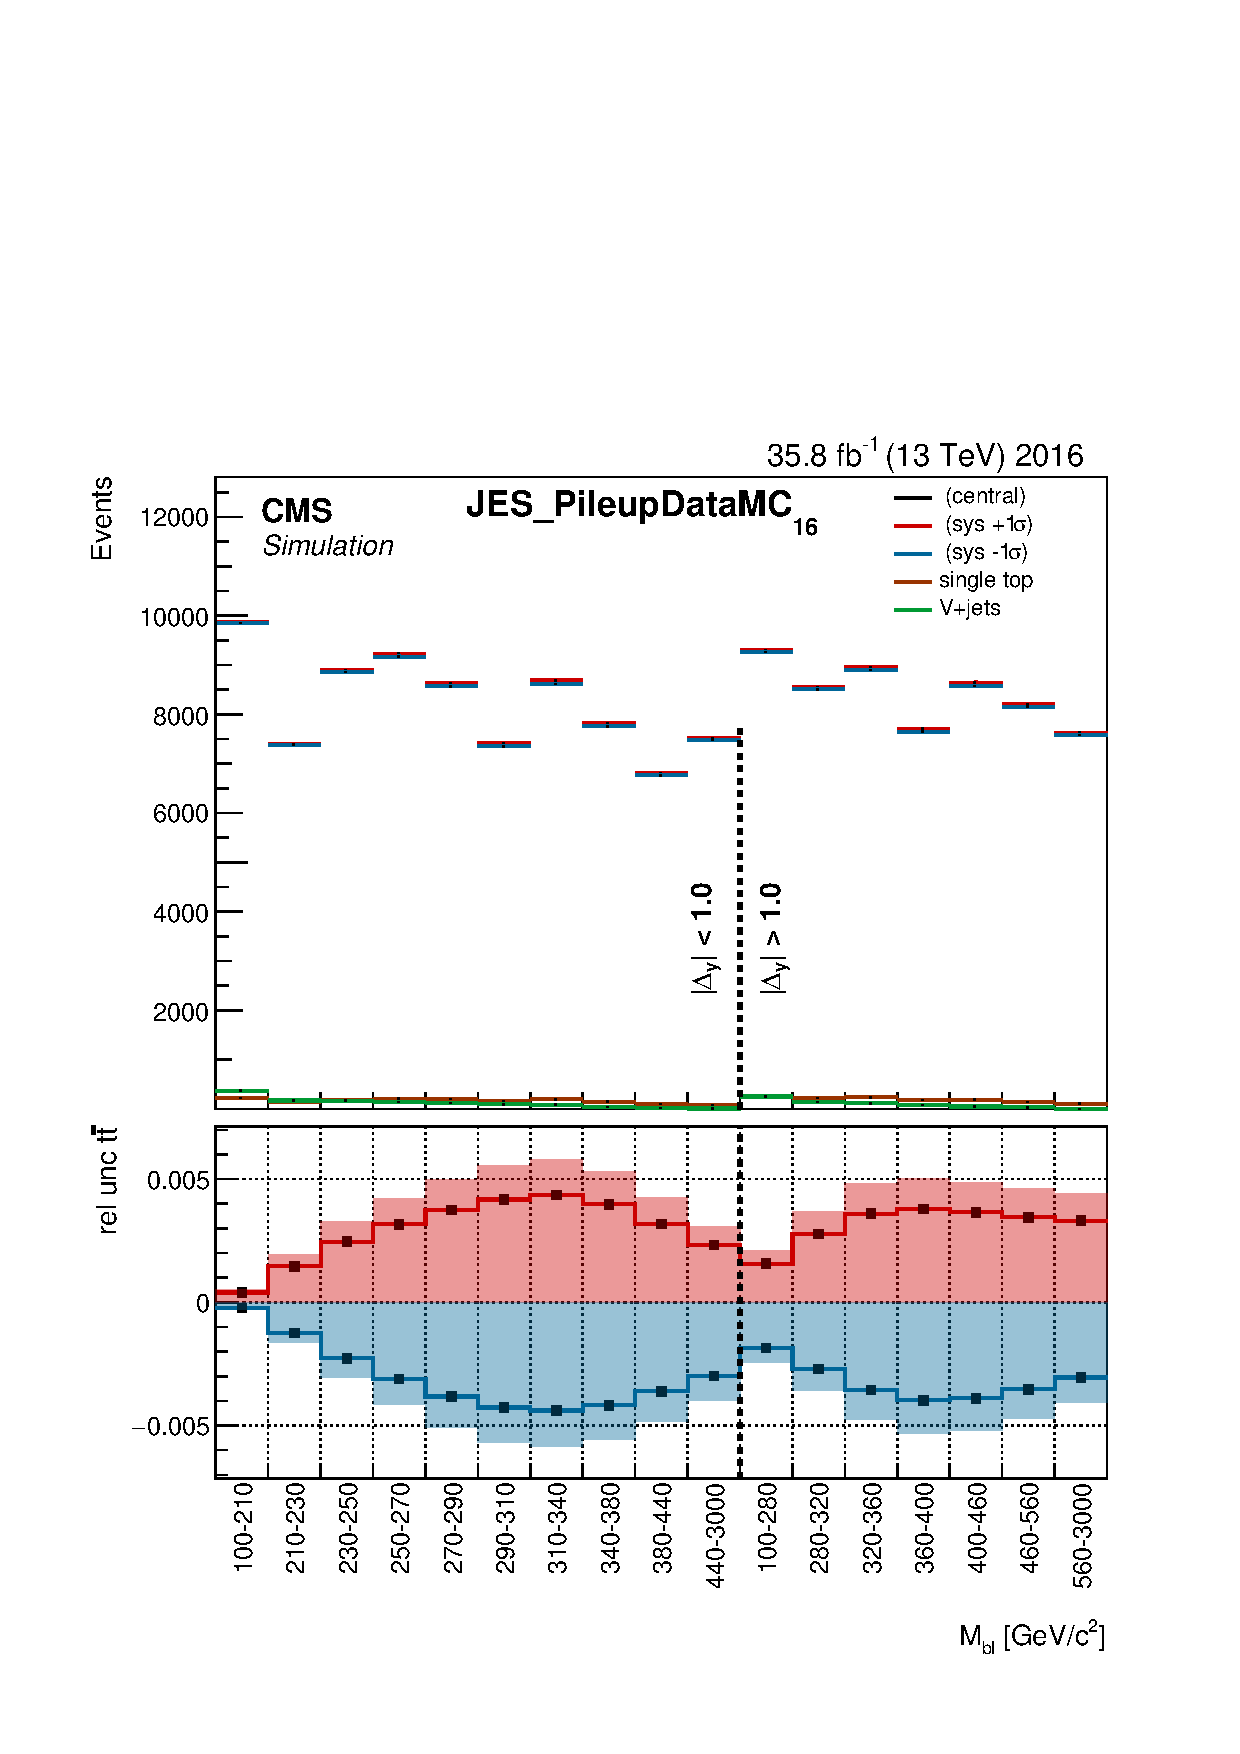
\includegraphics[width=.35\linewidth]{templates/JES_PileupDataMC_16}\hskip-.5cm
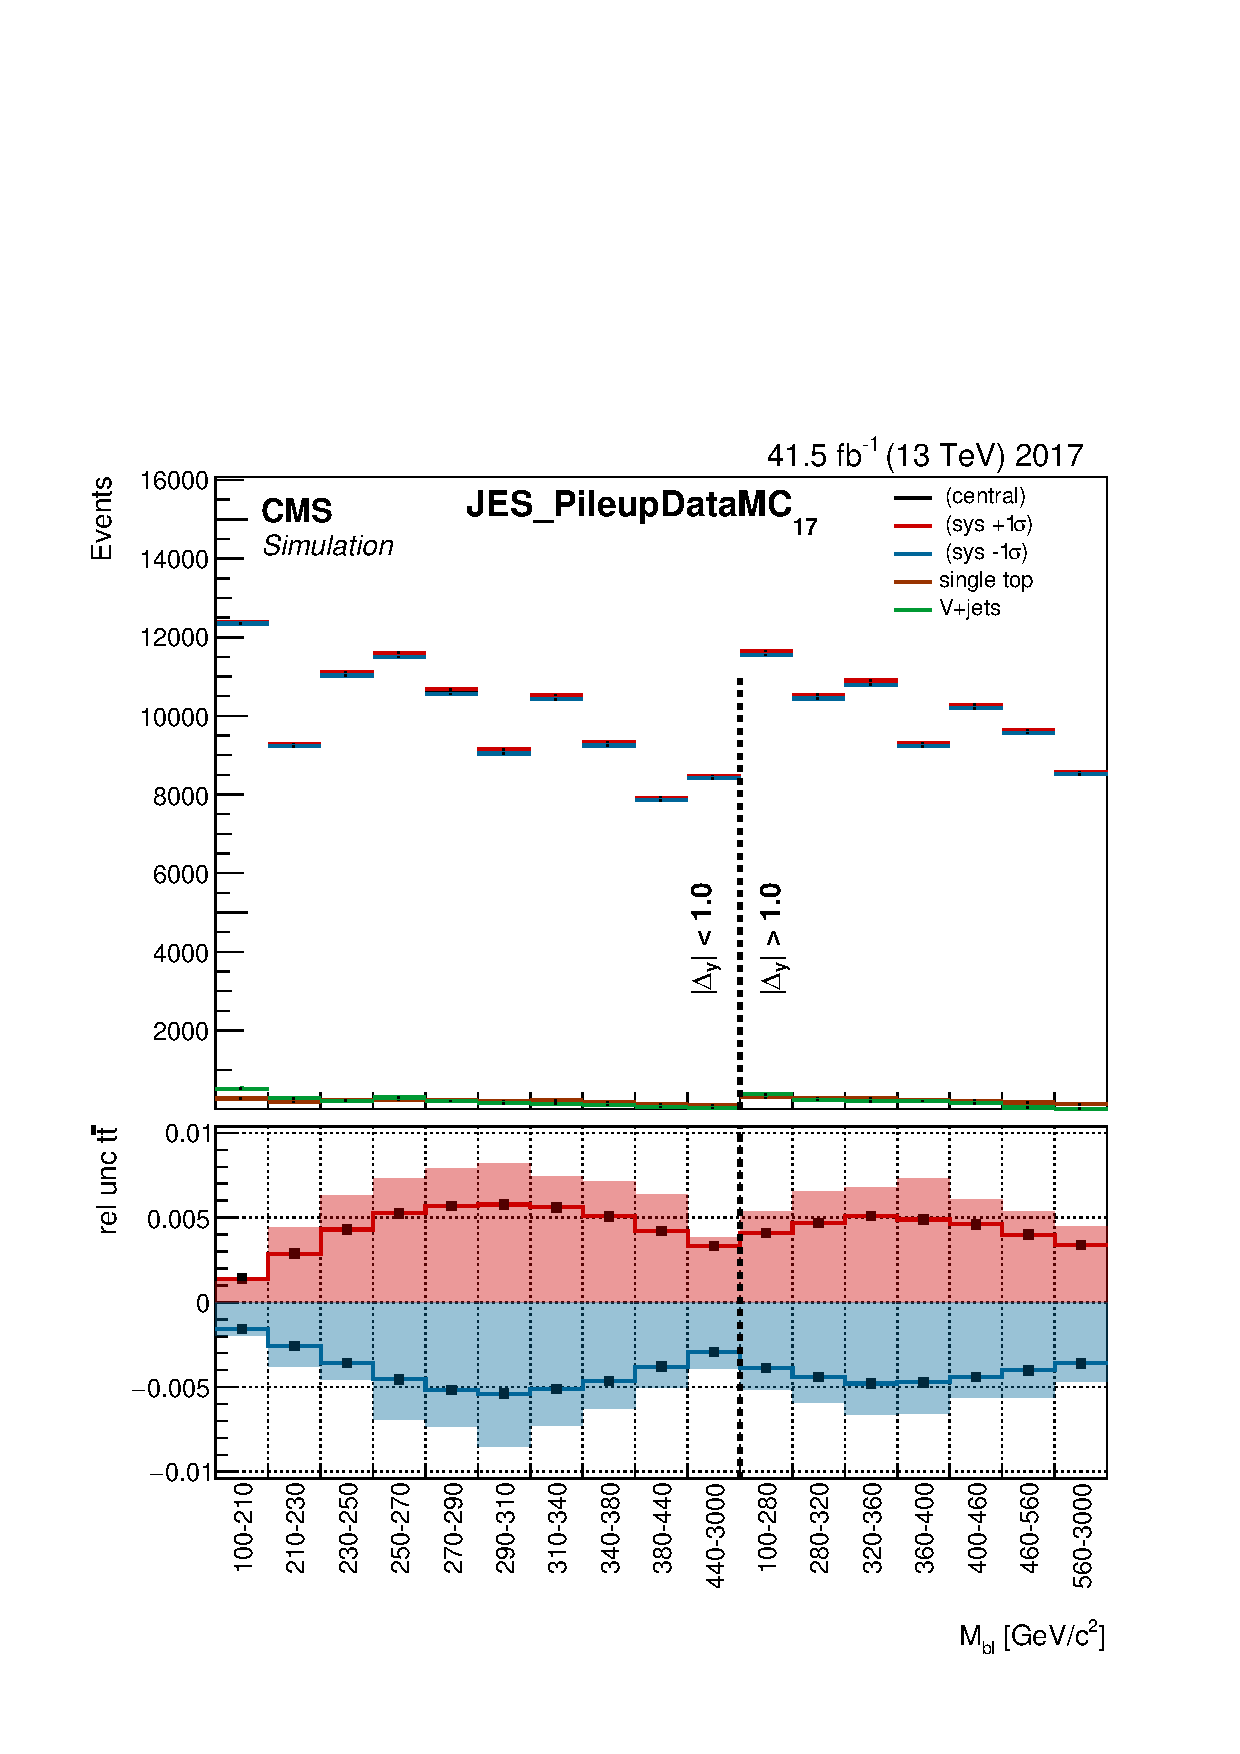
\includegraphics[width=.35\linewidth]{templates/JES_PileupDataMC_17}\hskip-.5cm
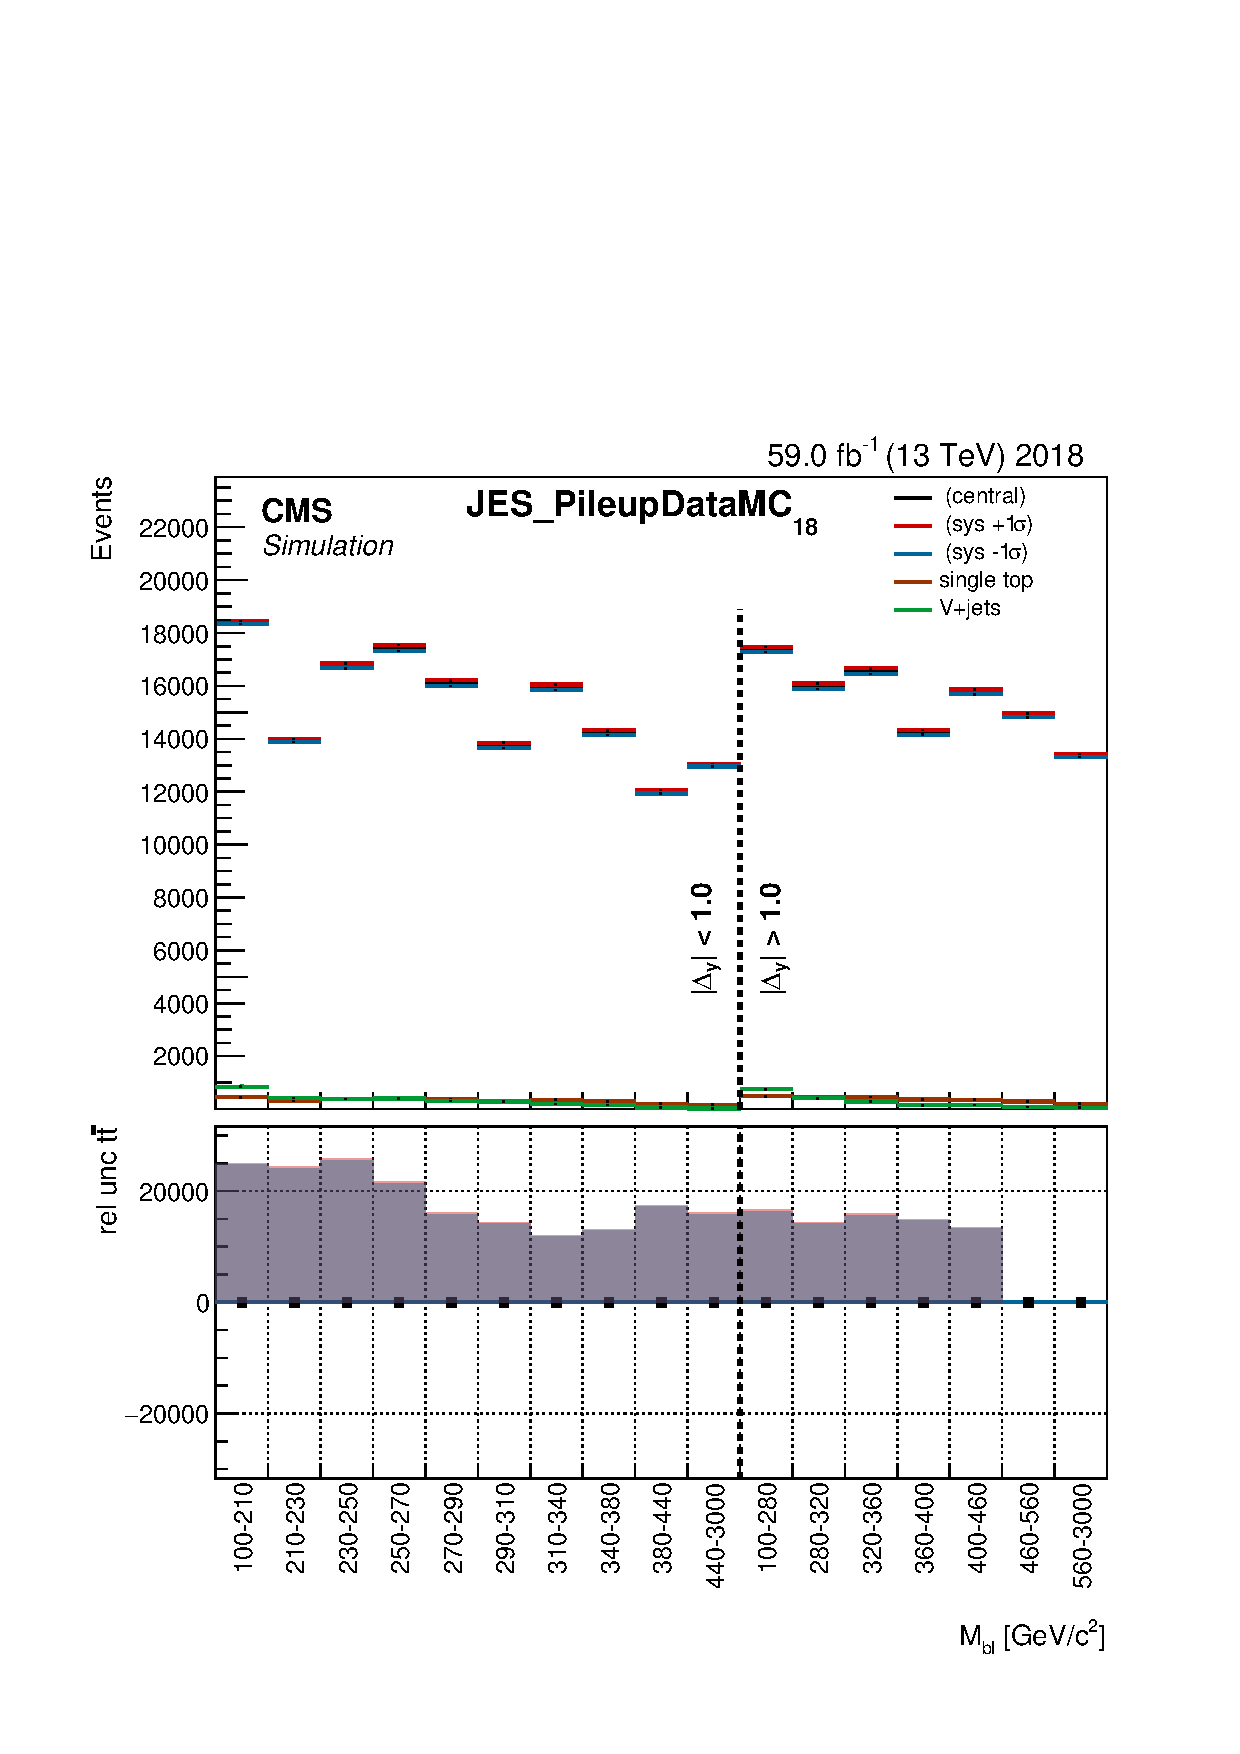
\includegraphics[width=.35\linewidth]{templates/JES_PileupDataMC_18}
\caption{JES\_PileupDataMC templates}
\label{fig:JES-PileupDataMC_template}
\end{figure}

\begin{figure} \centering
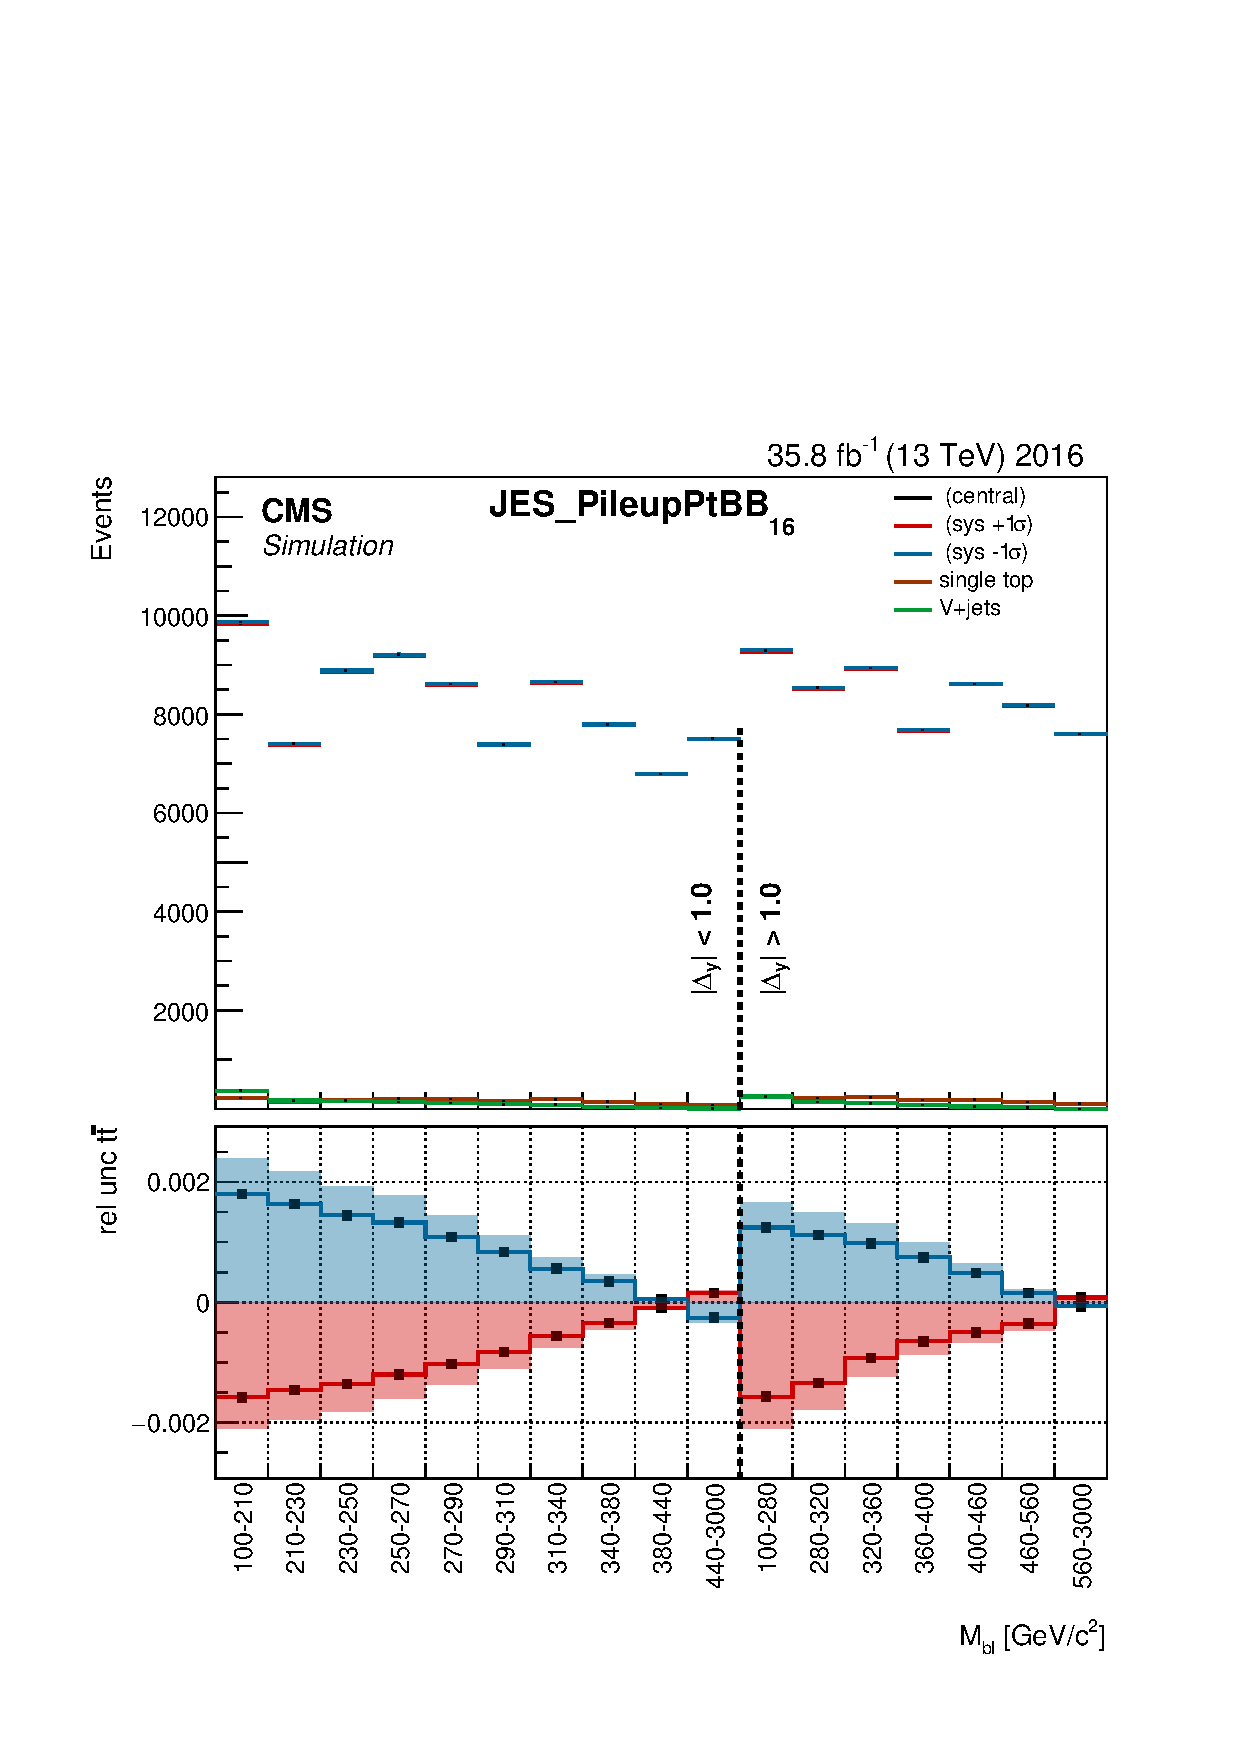
\includegraphics[width=.35\linewidth]{templates/JES_PileupPtBB_16}\hskip-.5cm
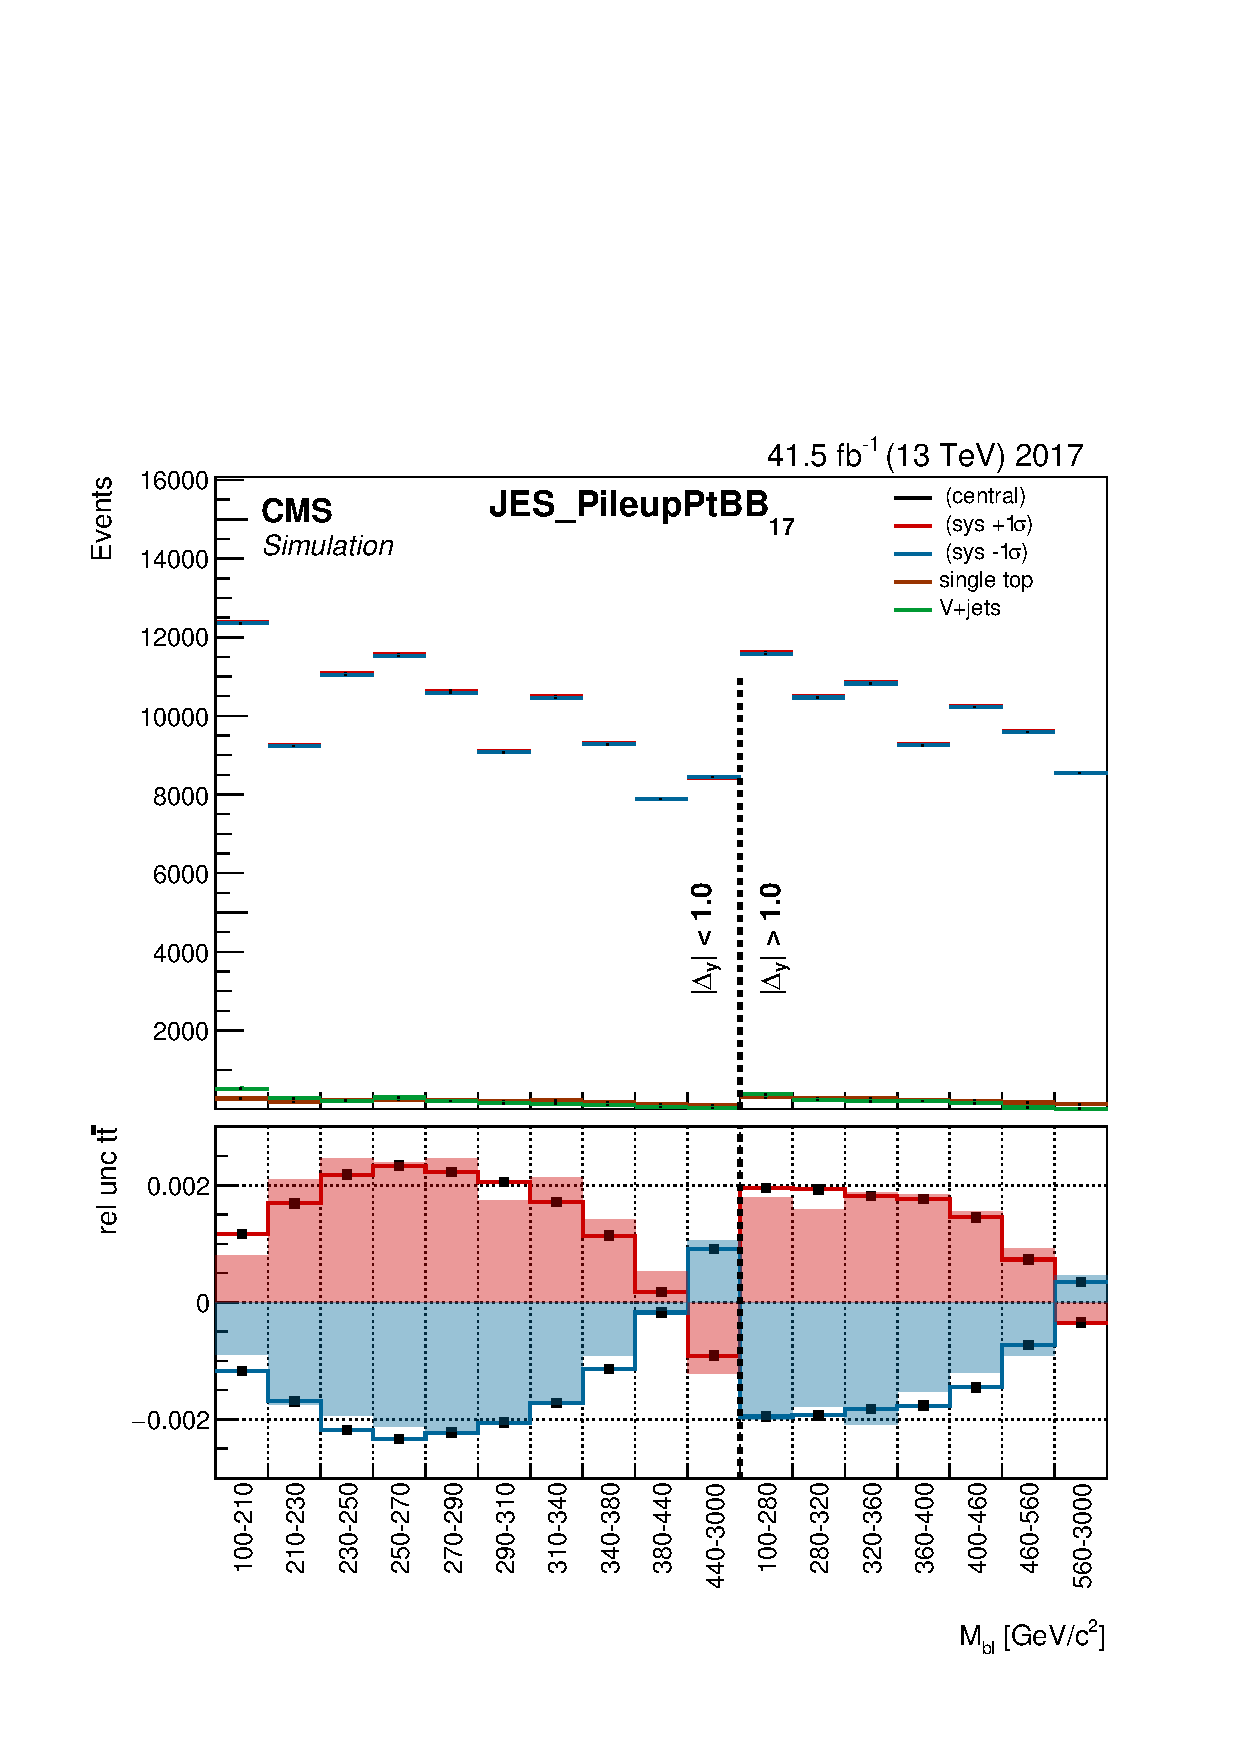
\includegraphics[width=.35\linewidth]{templates/JES_PileupPtBB_17}\hskip-.5cm
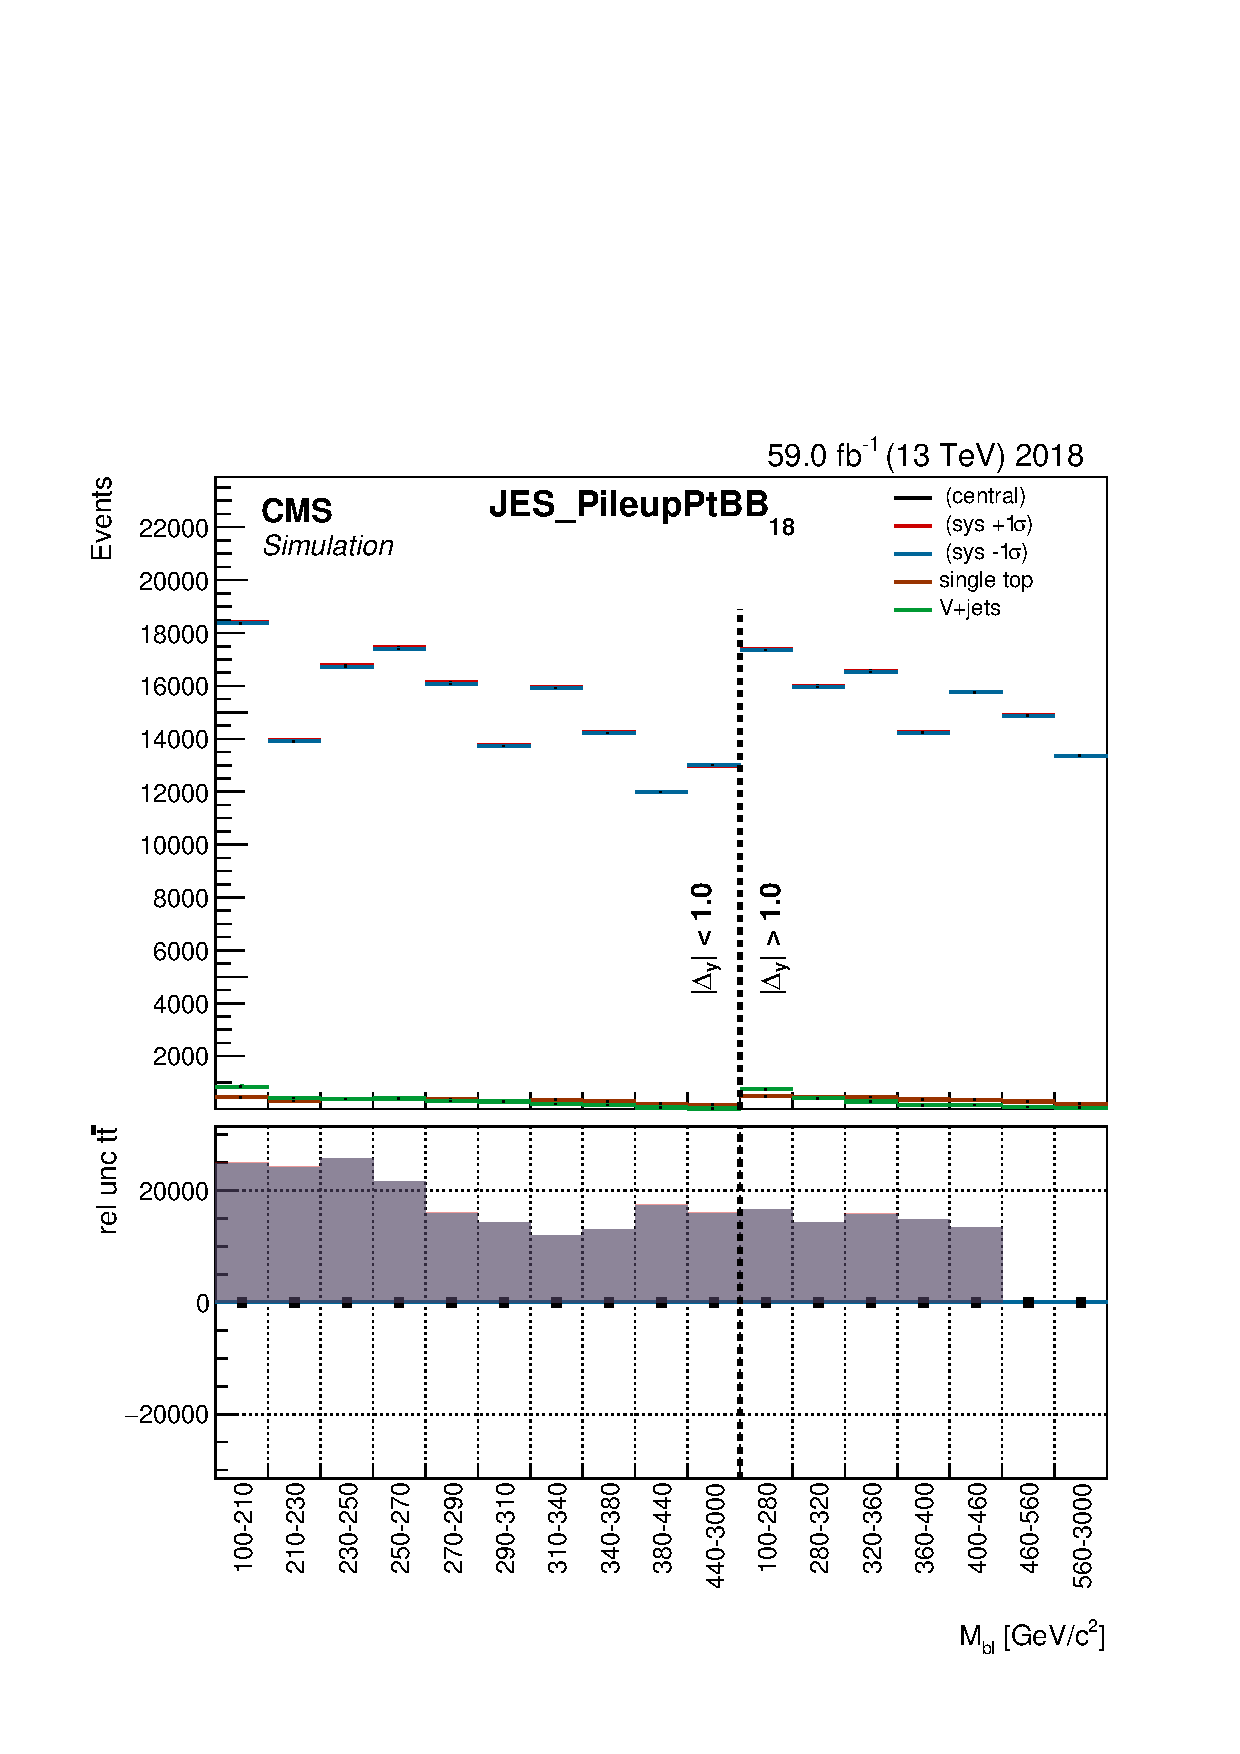
\includegraphics[width=.35\linewidth]{templates/JES_PileupPtBB_18}
\caption{JES\_PileupPtBB templates}
\label{fig:JES-PileupPtBB_template}
\end{figure}

\begin{figure} \centering
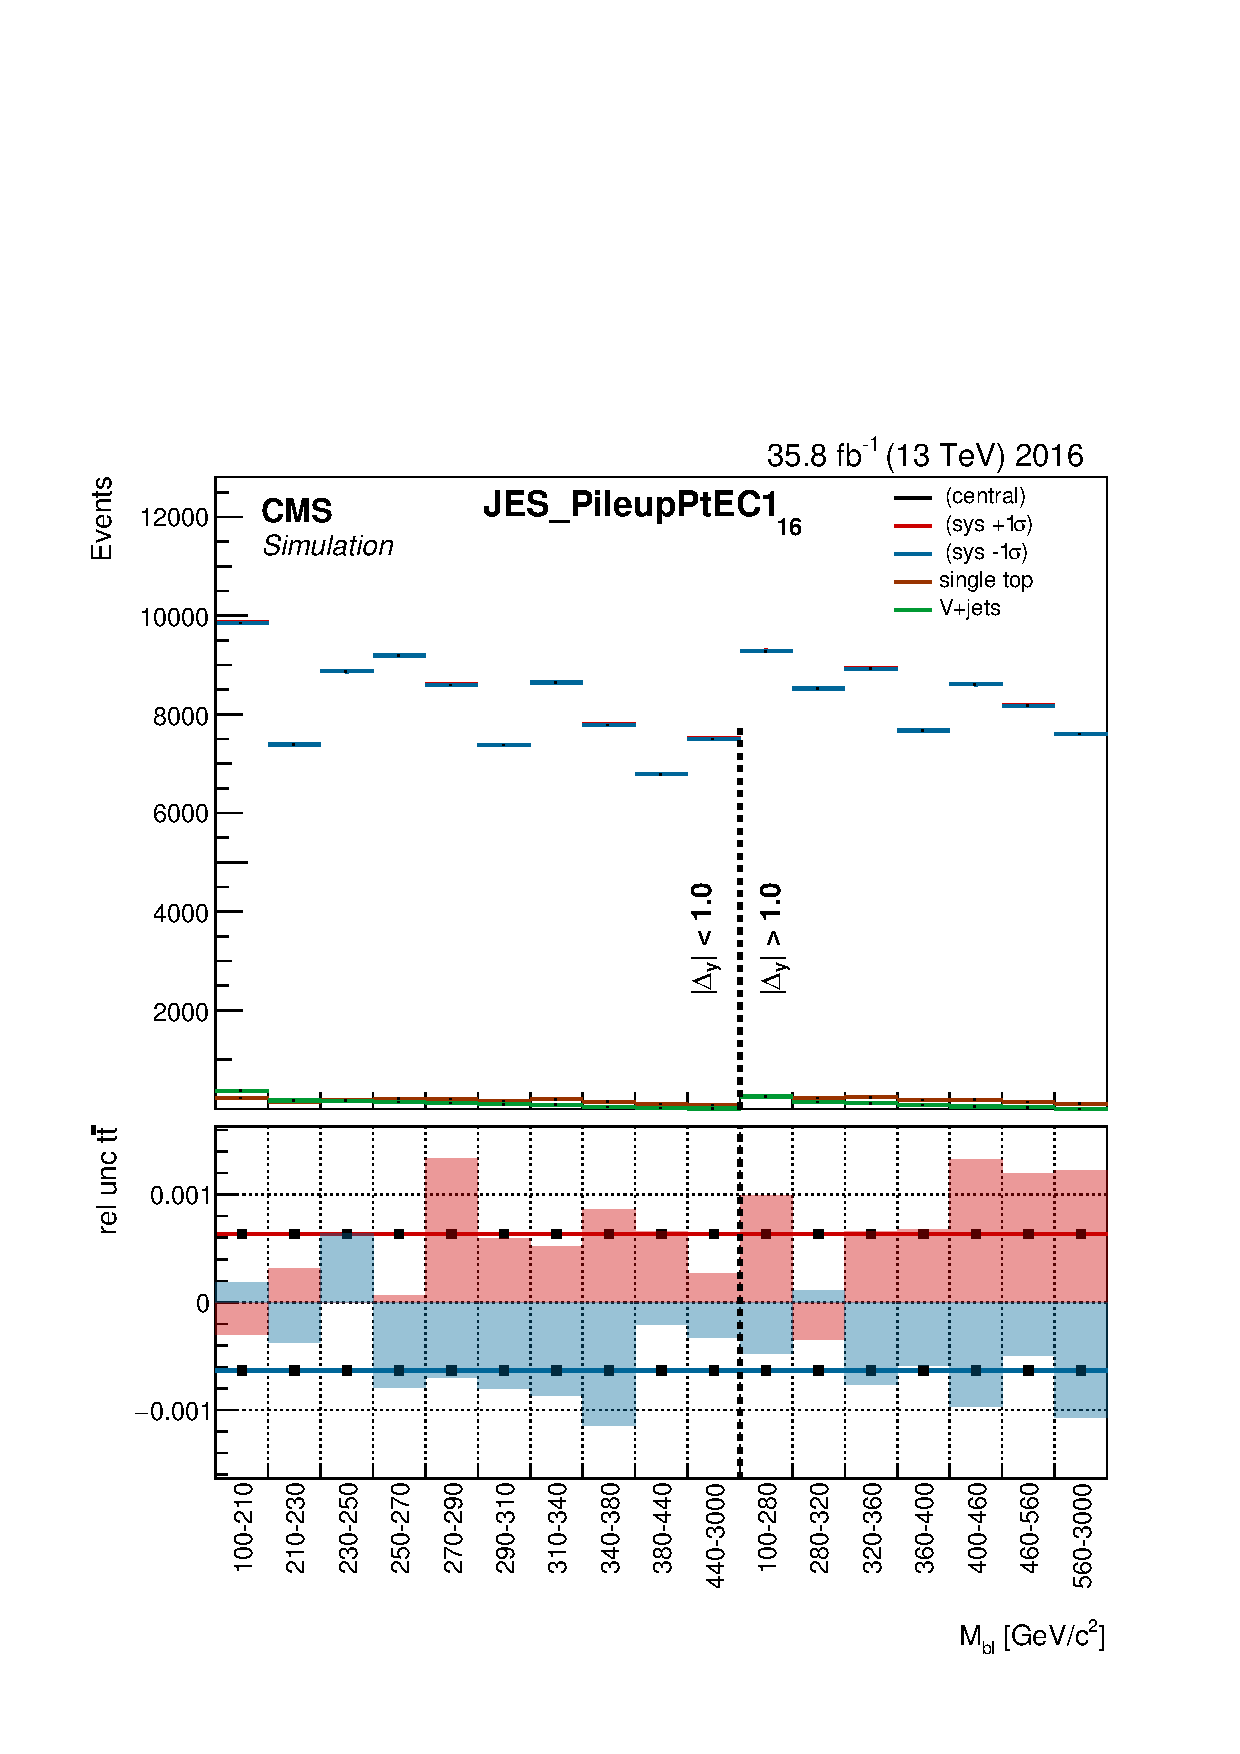
\includegraphics[width=.35\linewidth]{templates/JES_PileupPtEC1_16}\hskip-.5cm
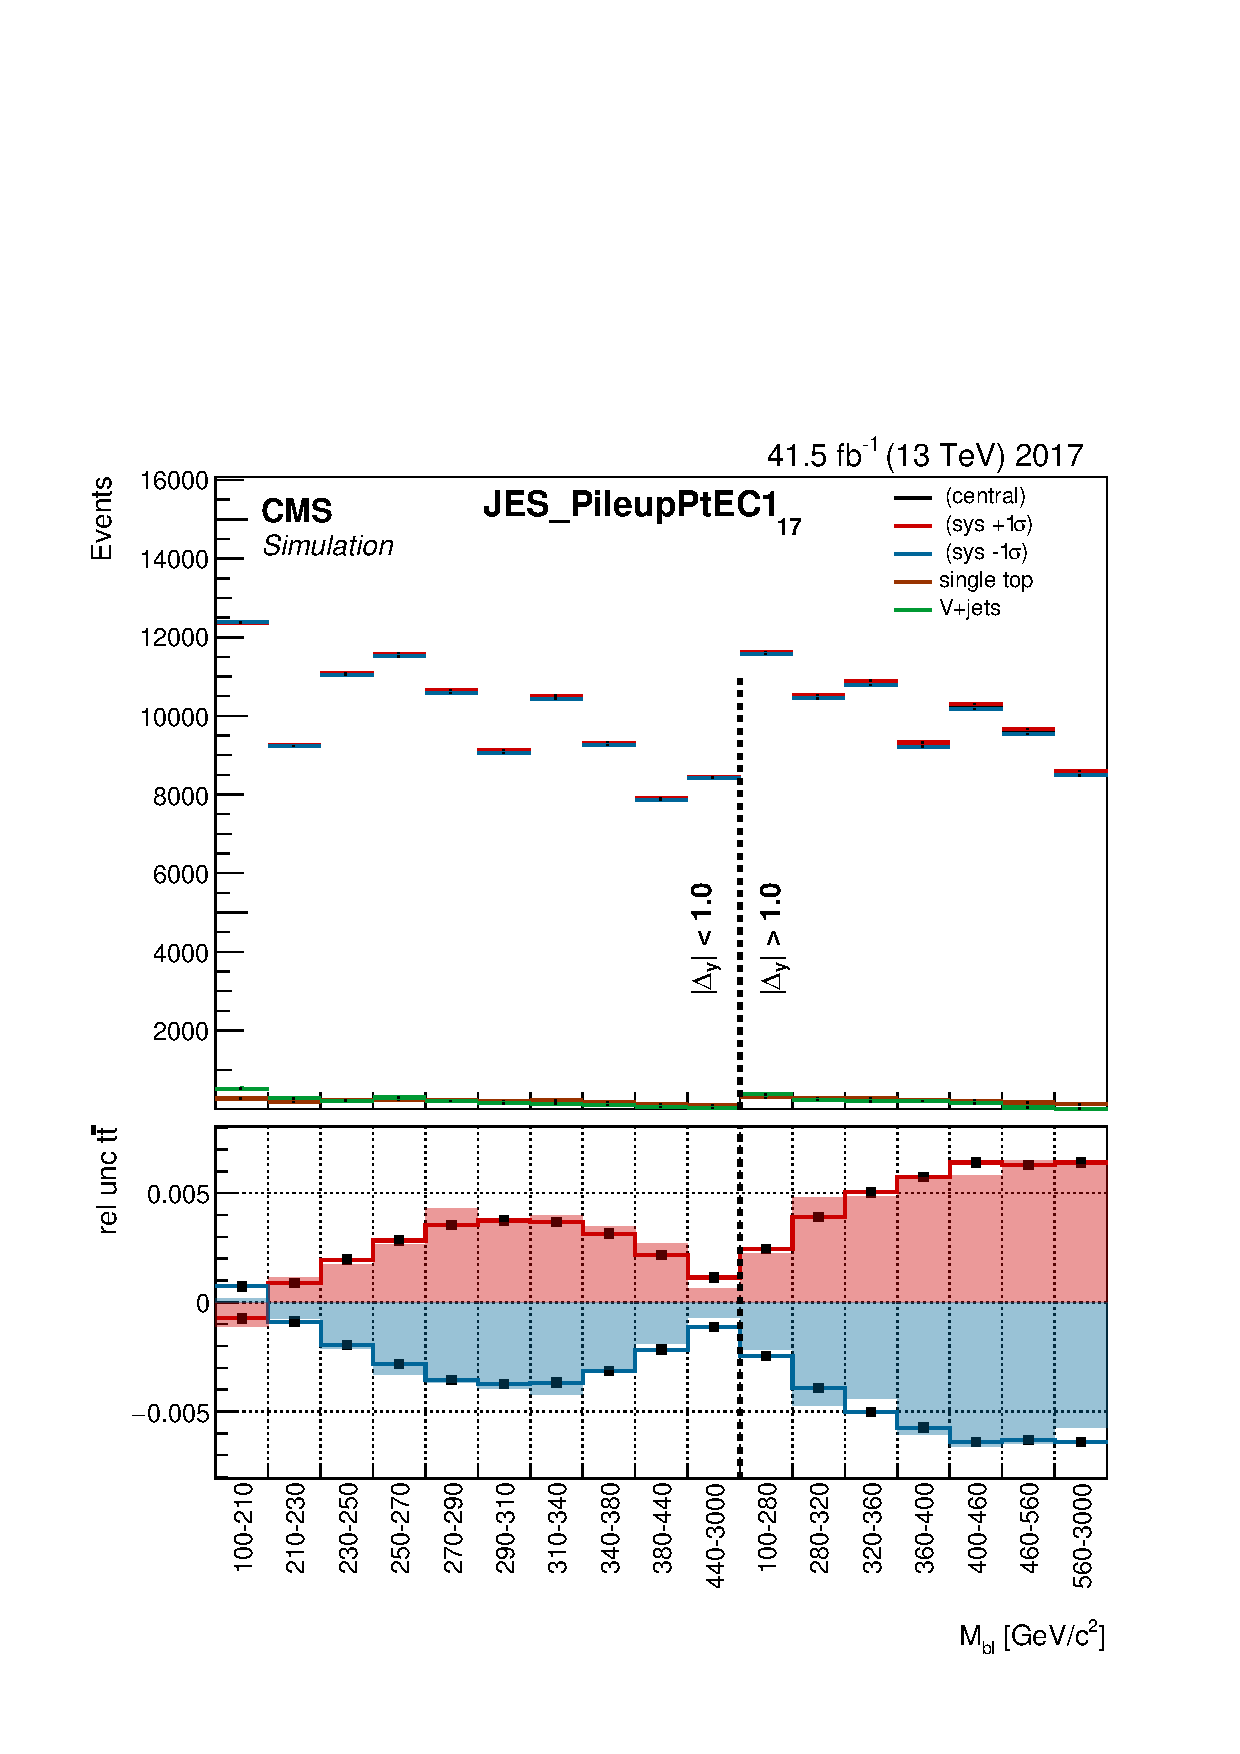
\includegraphics[width=.35\linewidth]{templates/JES_PileupPtEC1_17}\hskip-.5cm
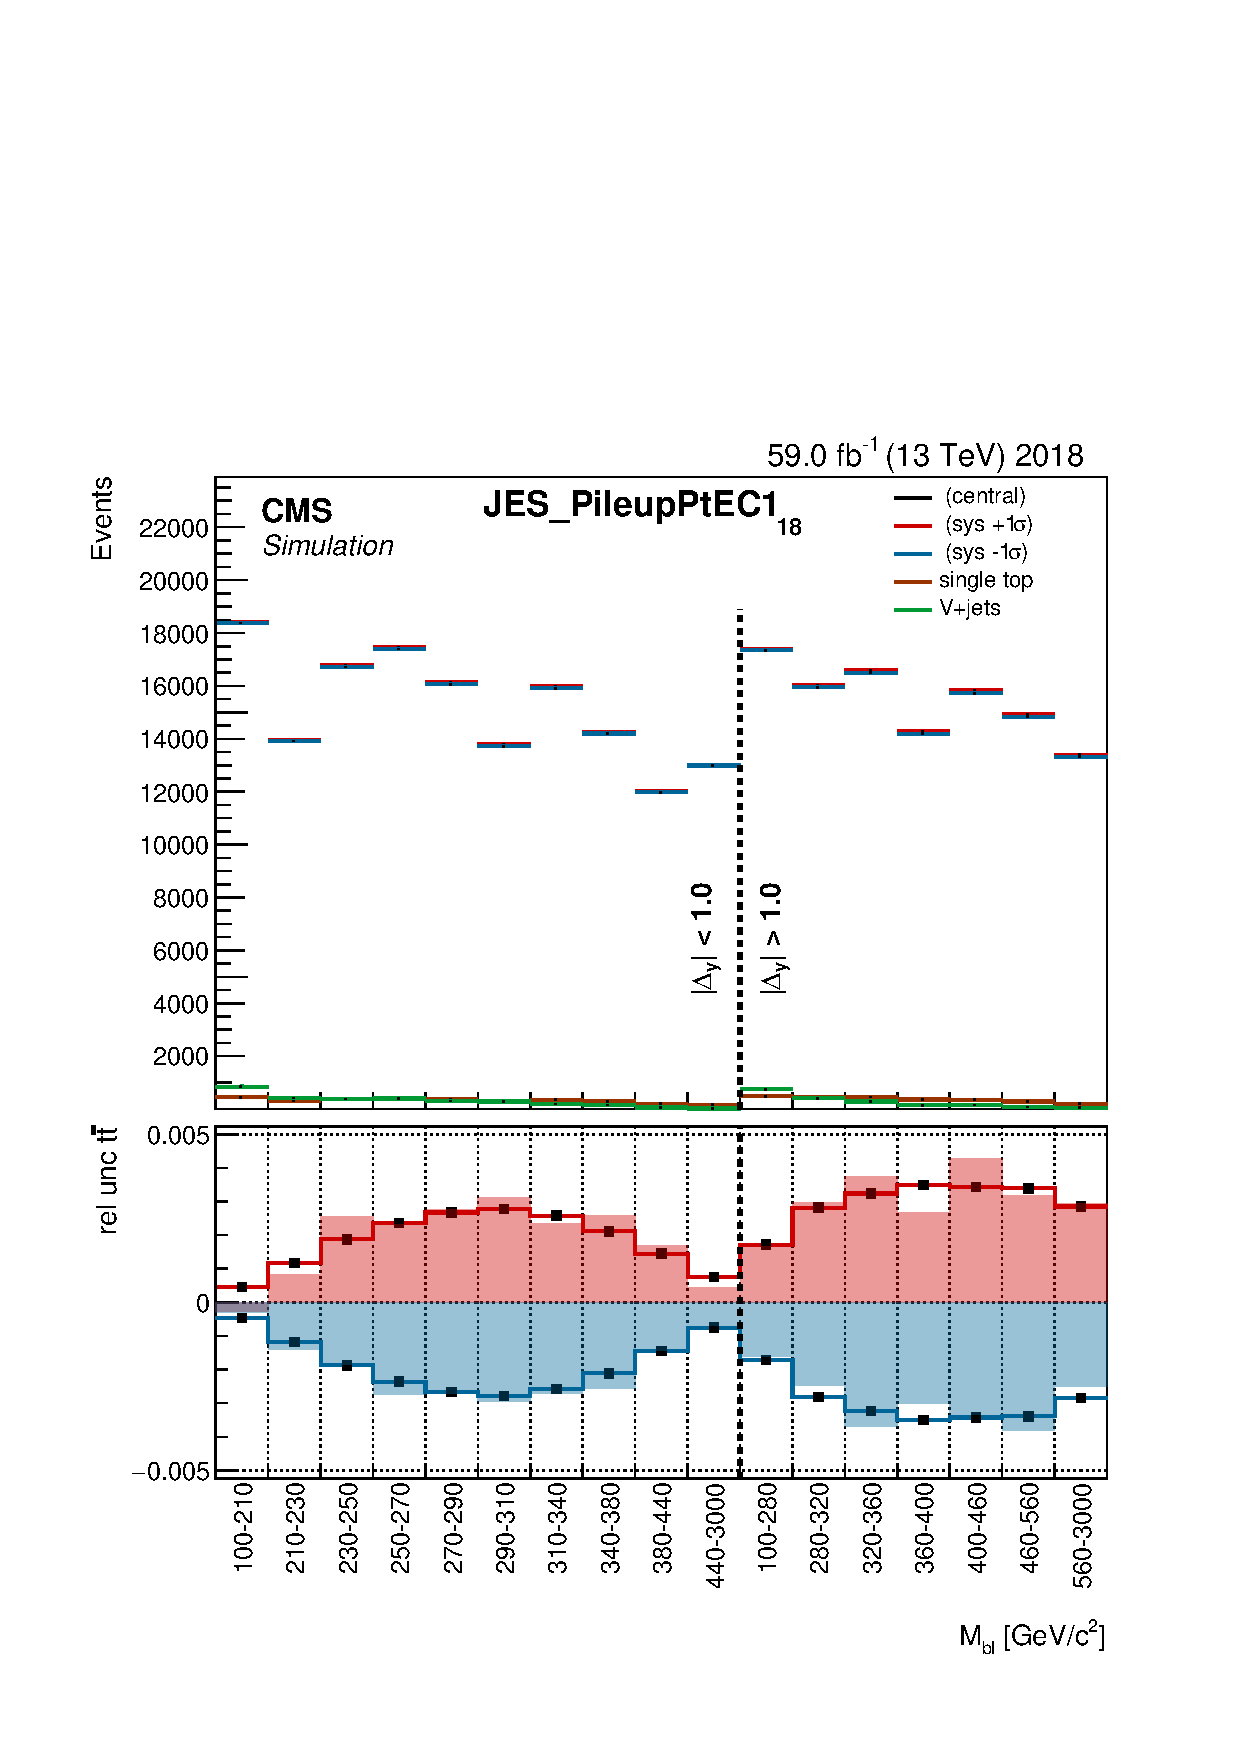
\includegraphics[width=.35\linewidth]{templates/JES_PileupPtEC1_18}
\caption{JES\_PileupPtEC1 templates}
\label{fig:JES-PileupPtEC1_template}
\end{figure}

\begin{figure} \centering
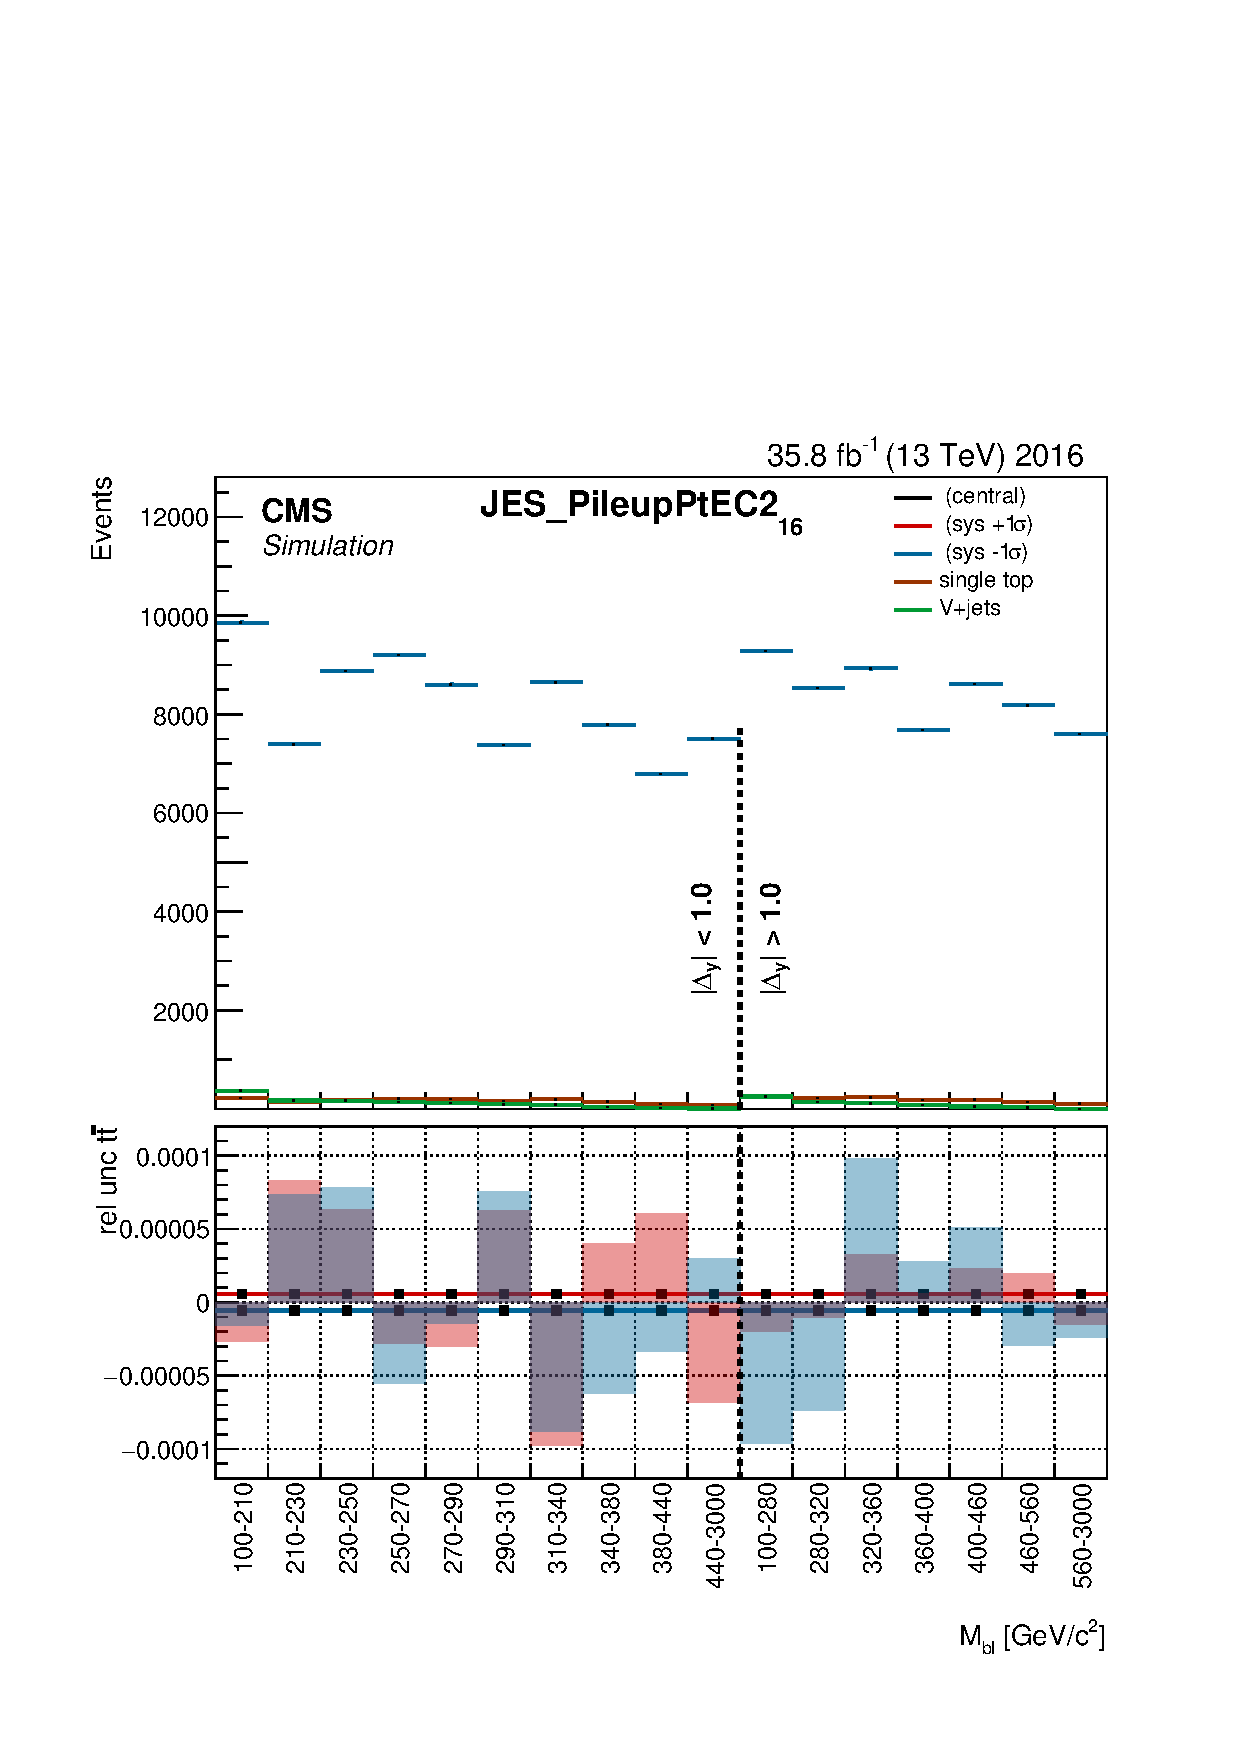
\includegraphics[width=.35\linewidth]{templates/JES_PileupPtEC2_16}\hskip-.5cm
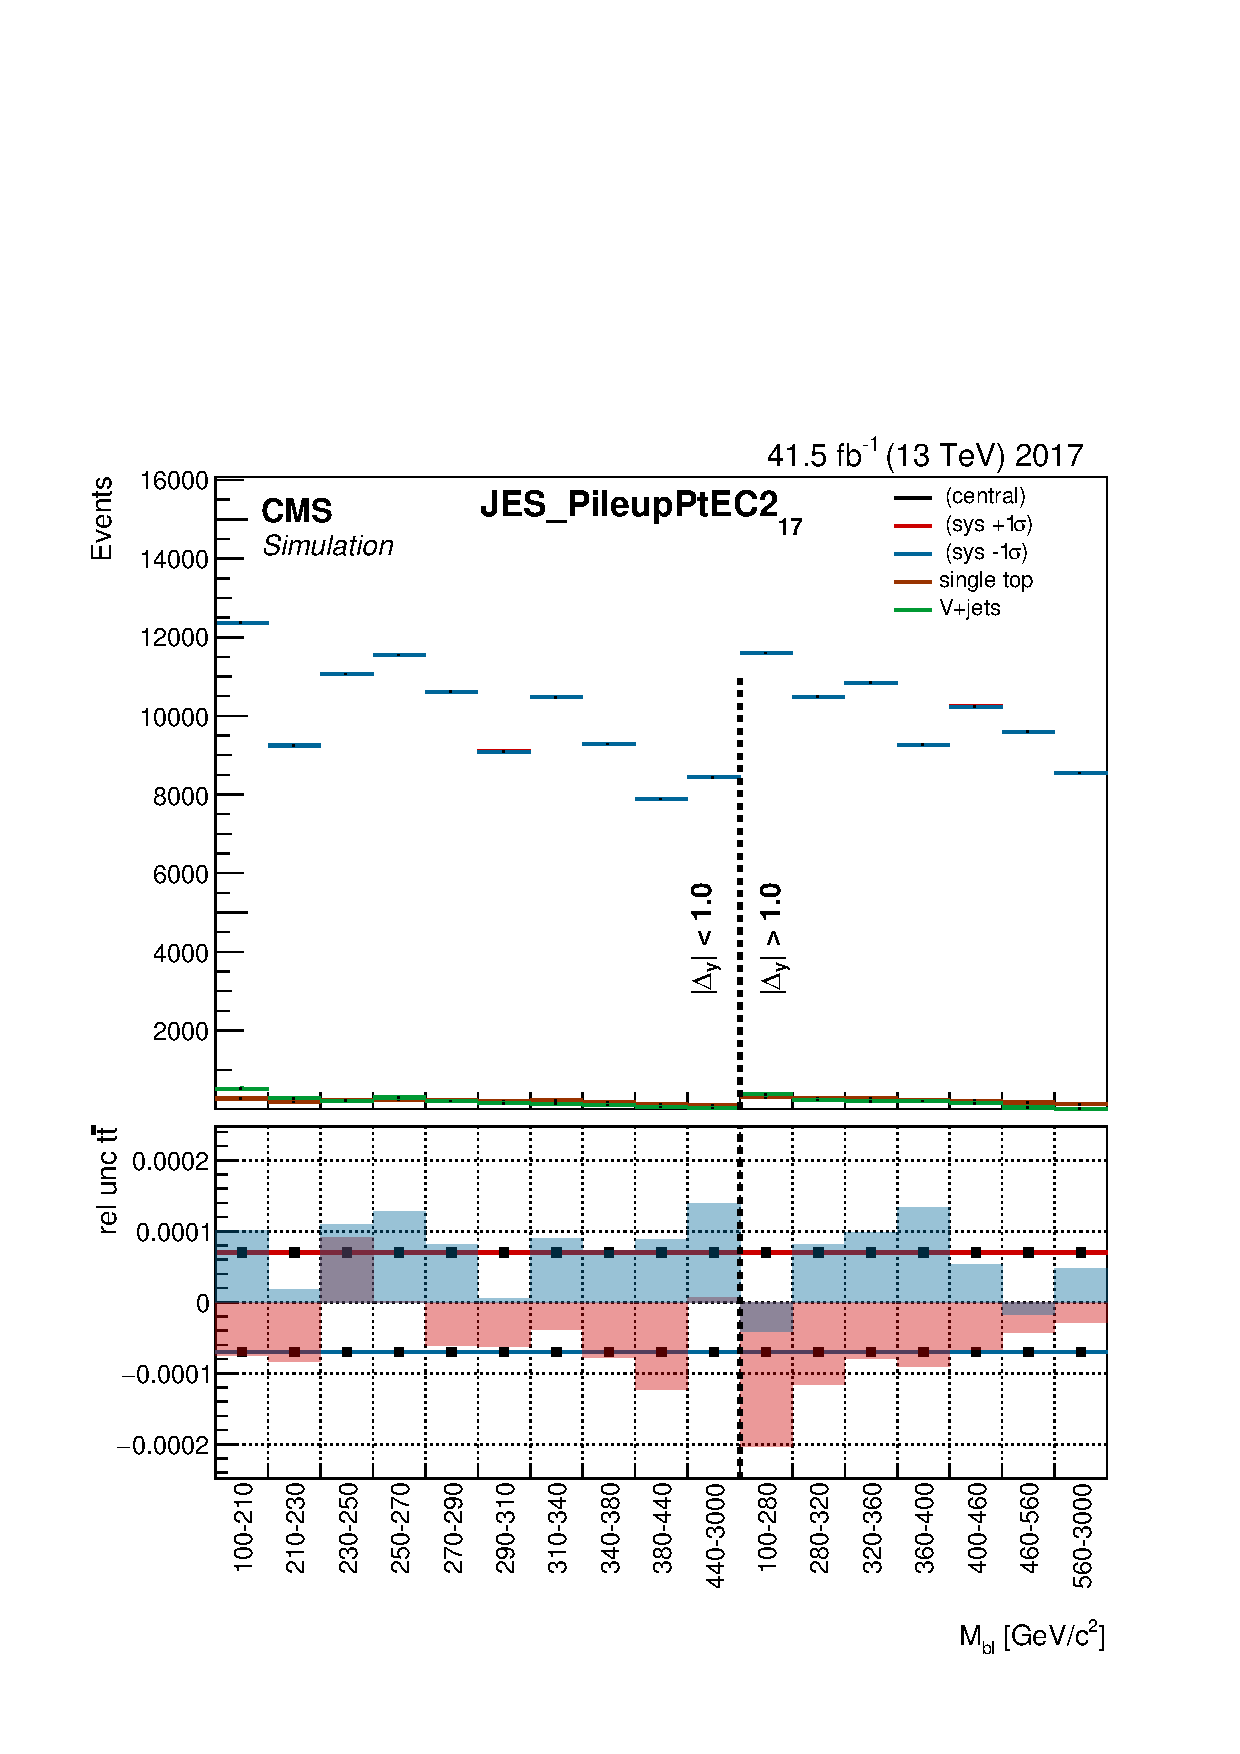
\includegraphics[width=.35\linewidth]{templates/JES_PileupPtEC2_17}\hskip-.5cm
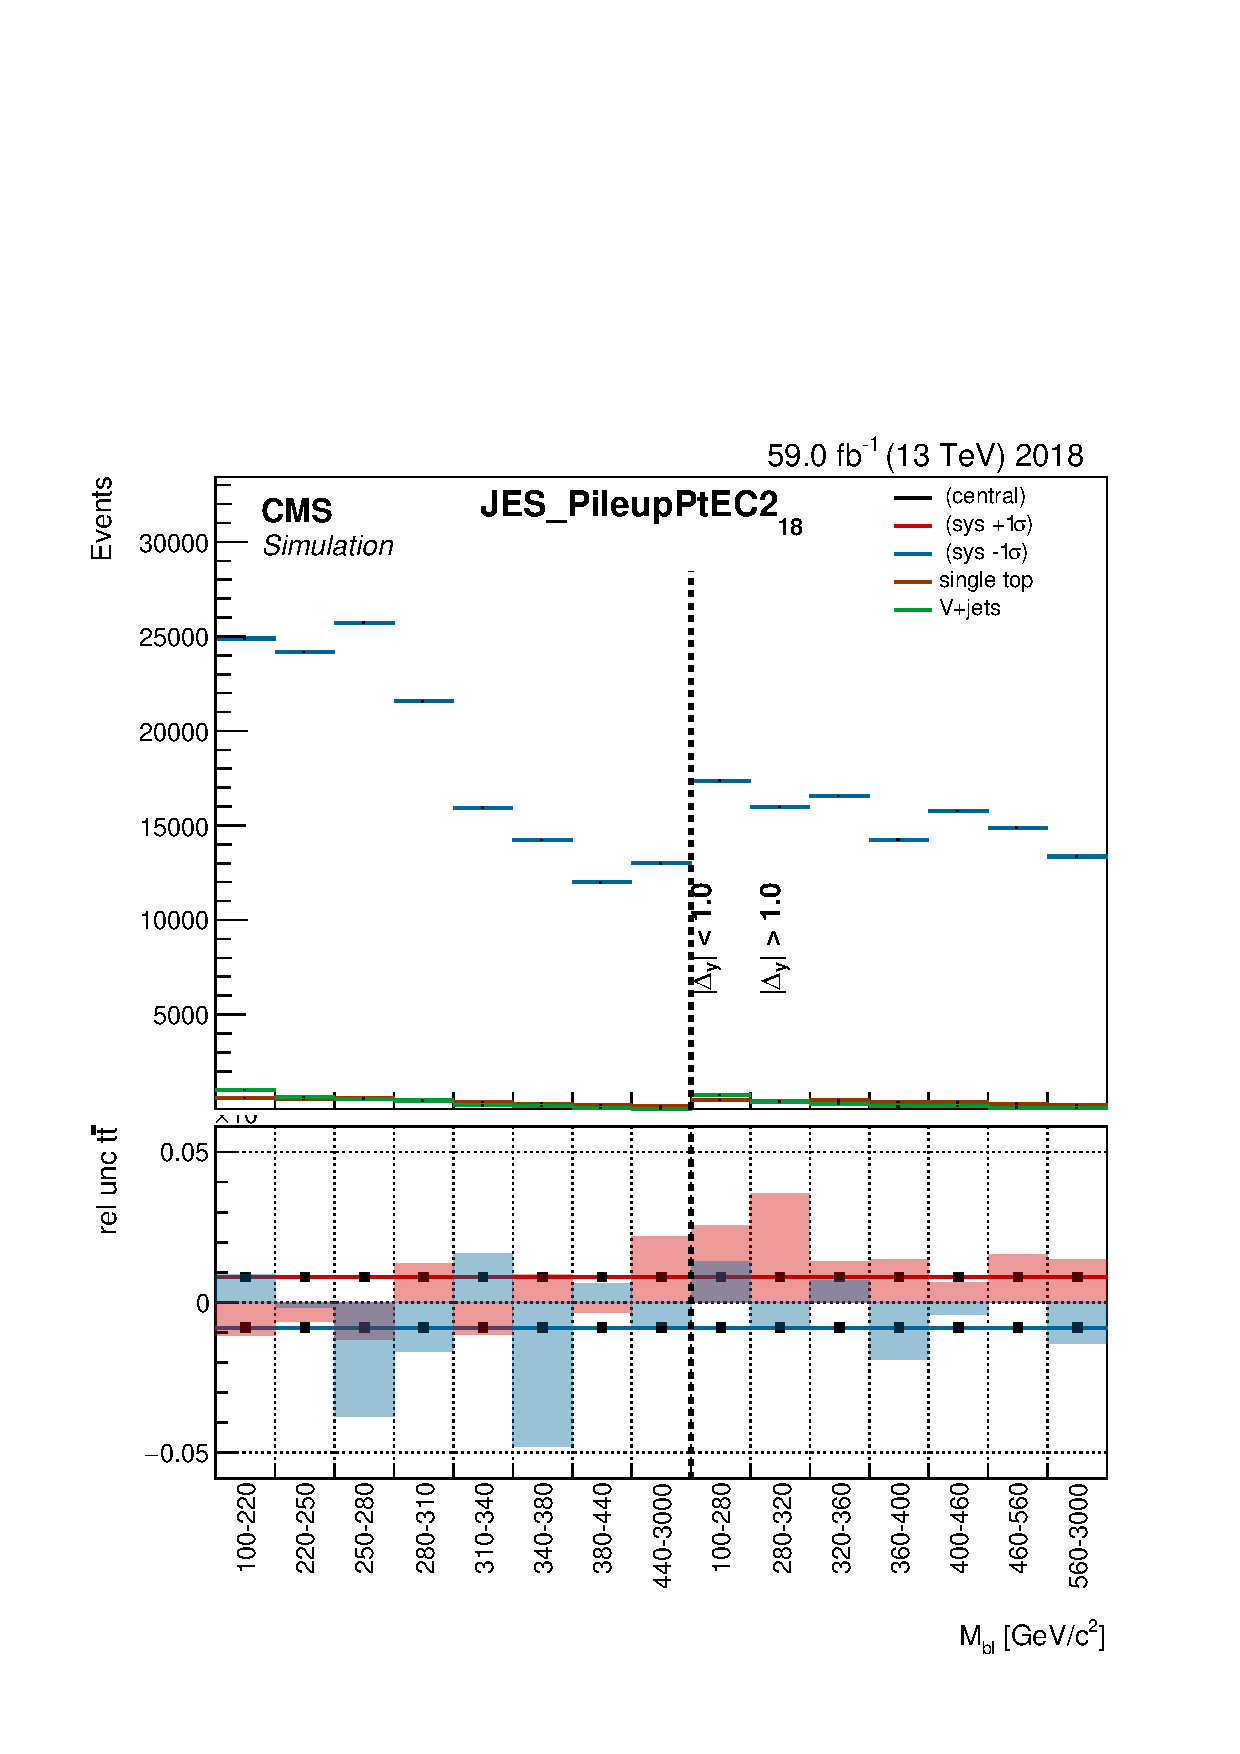
\includegraphics[width=.35\linewidth]{templates/JES_PileupPtEC2_18}
\caption{JES\_PileupPtEC2 templates}
\label{fig:JES-PileupPtEC2_template}
\end{figure}

\begin{figure} \centering
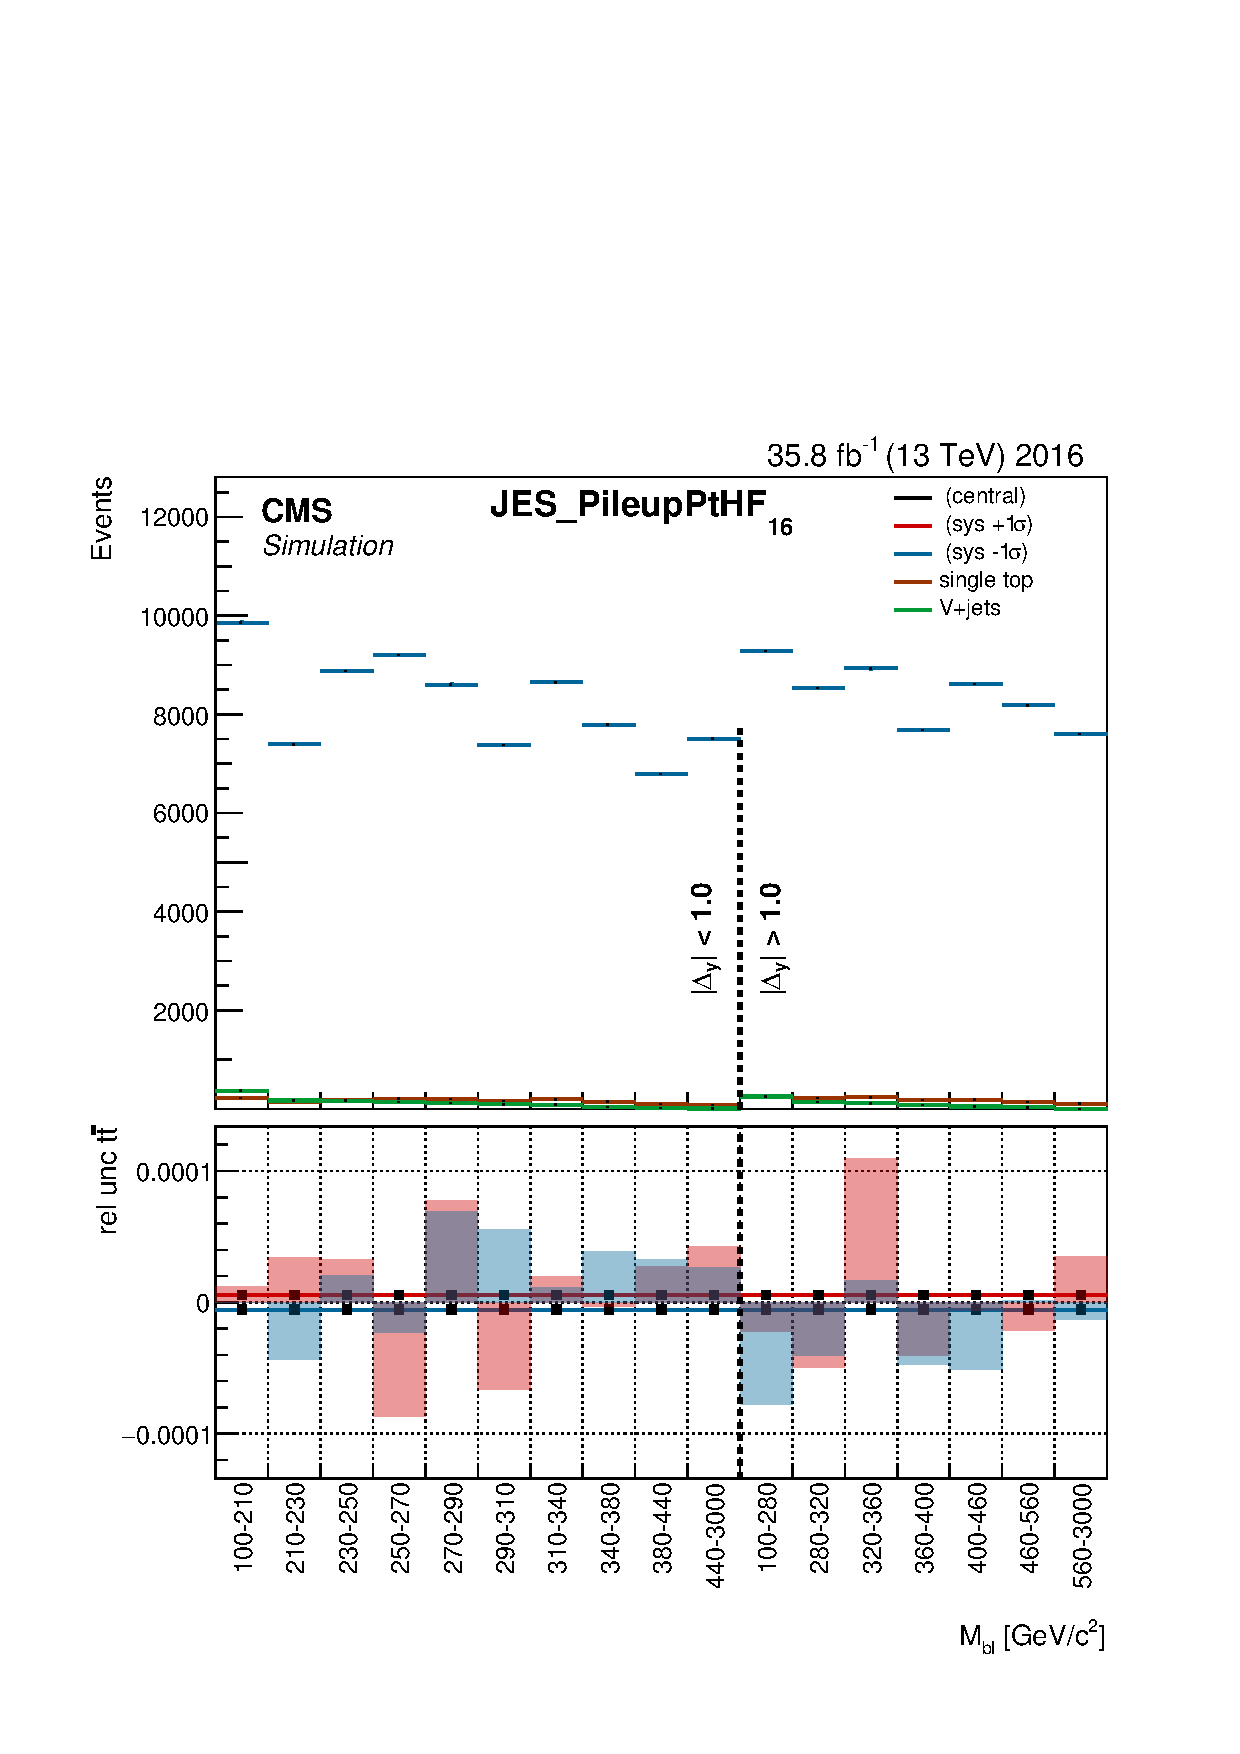
\includegraphics[width=.35\linewidth]{templates/JES_PileupPtHF_16}\hskip-.5cm
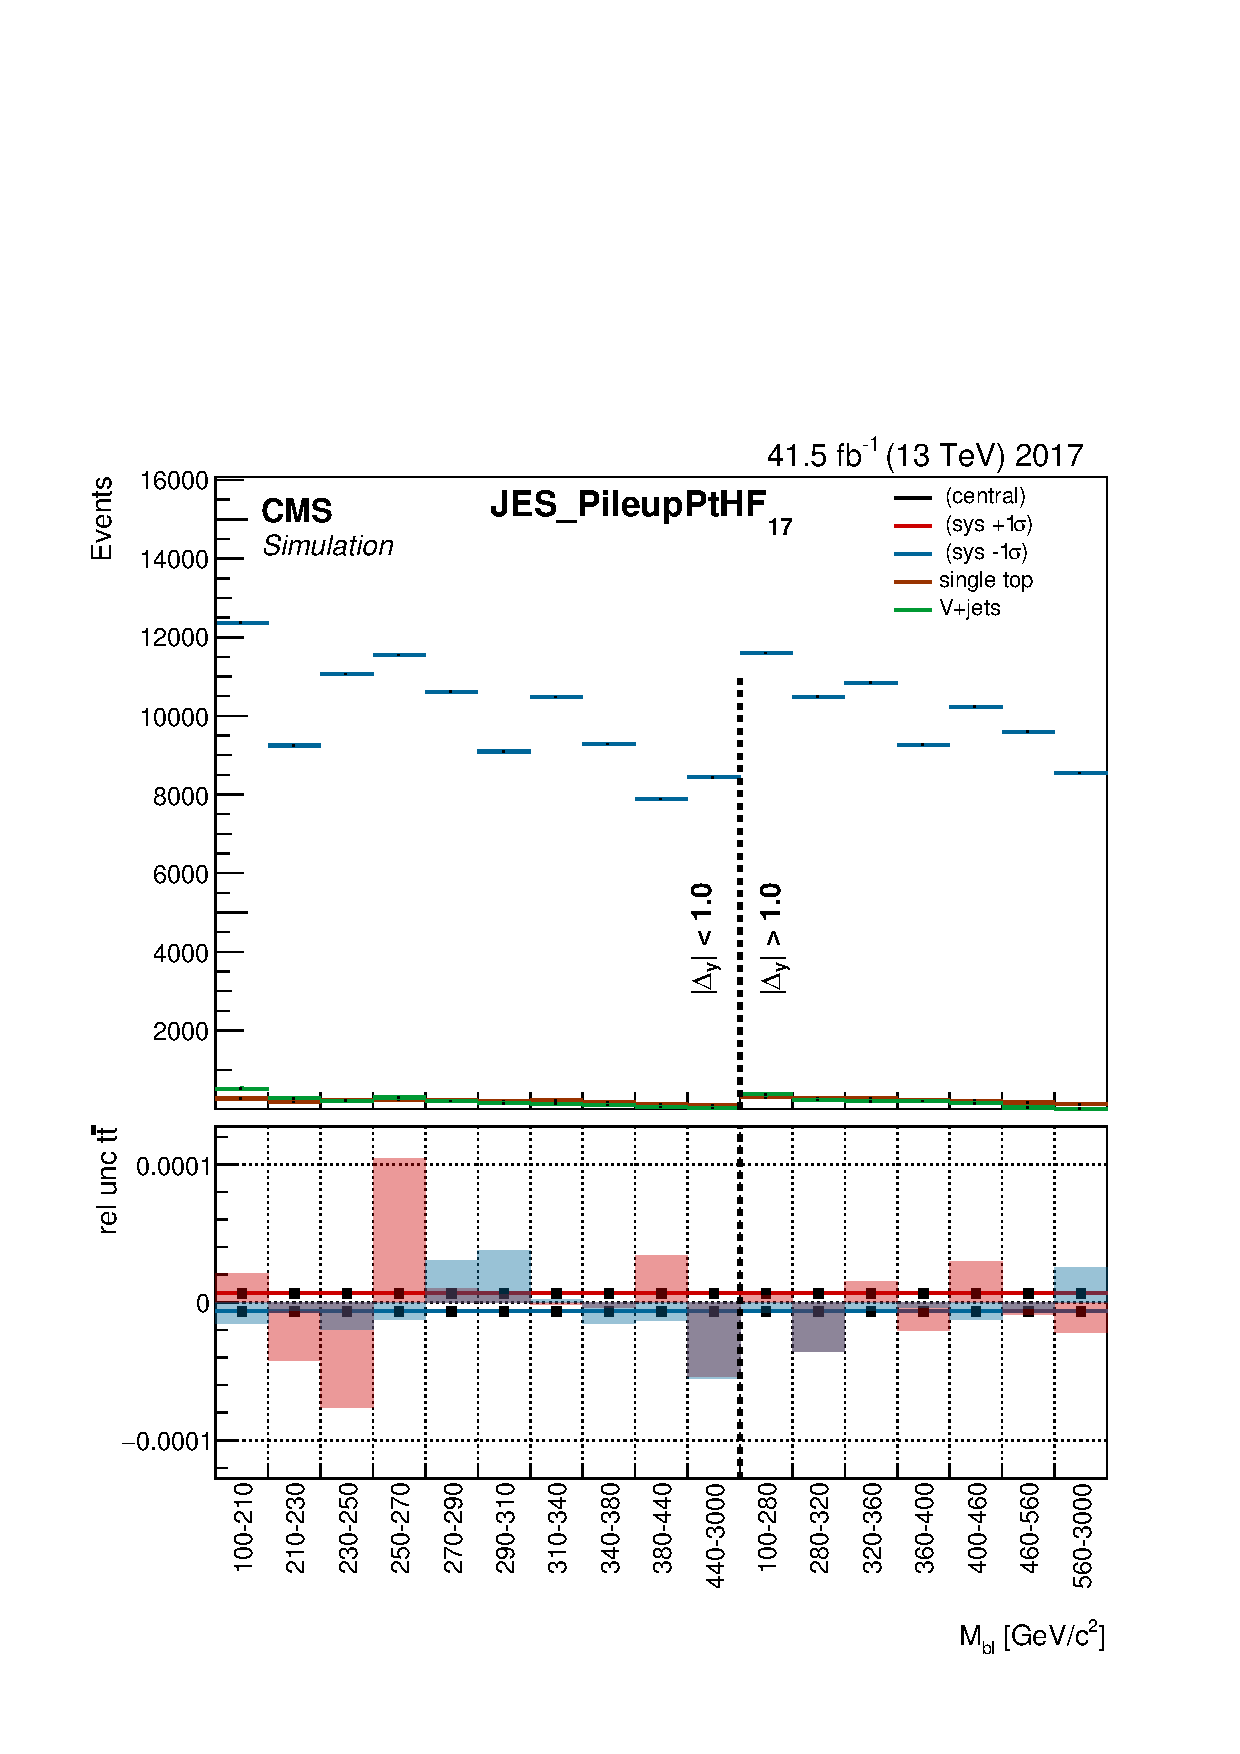
\includegraphics[width=.35\linewidth]{templates/JES_PileupPtHF_17}\hskip-.5cm
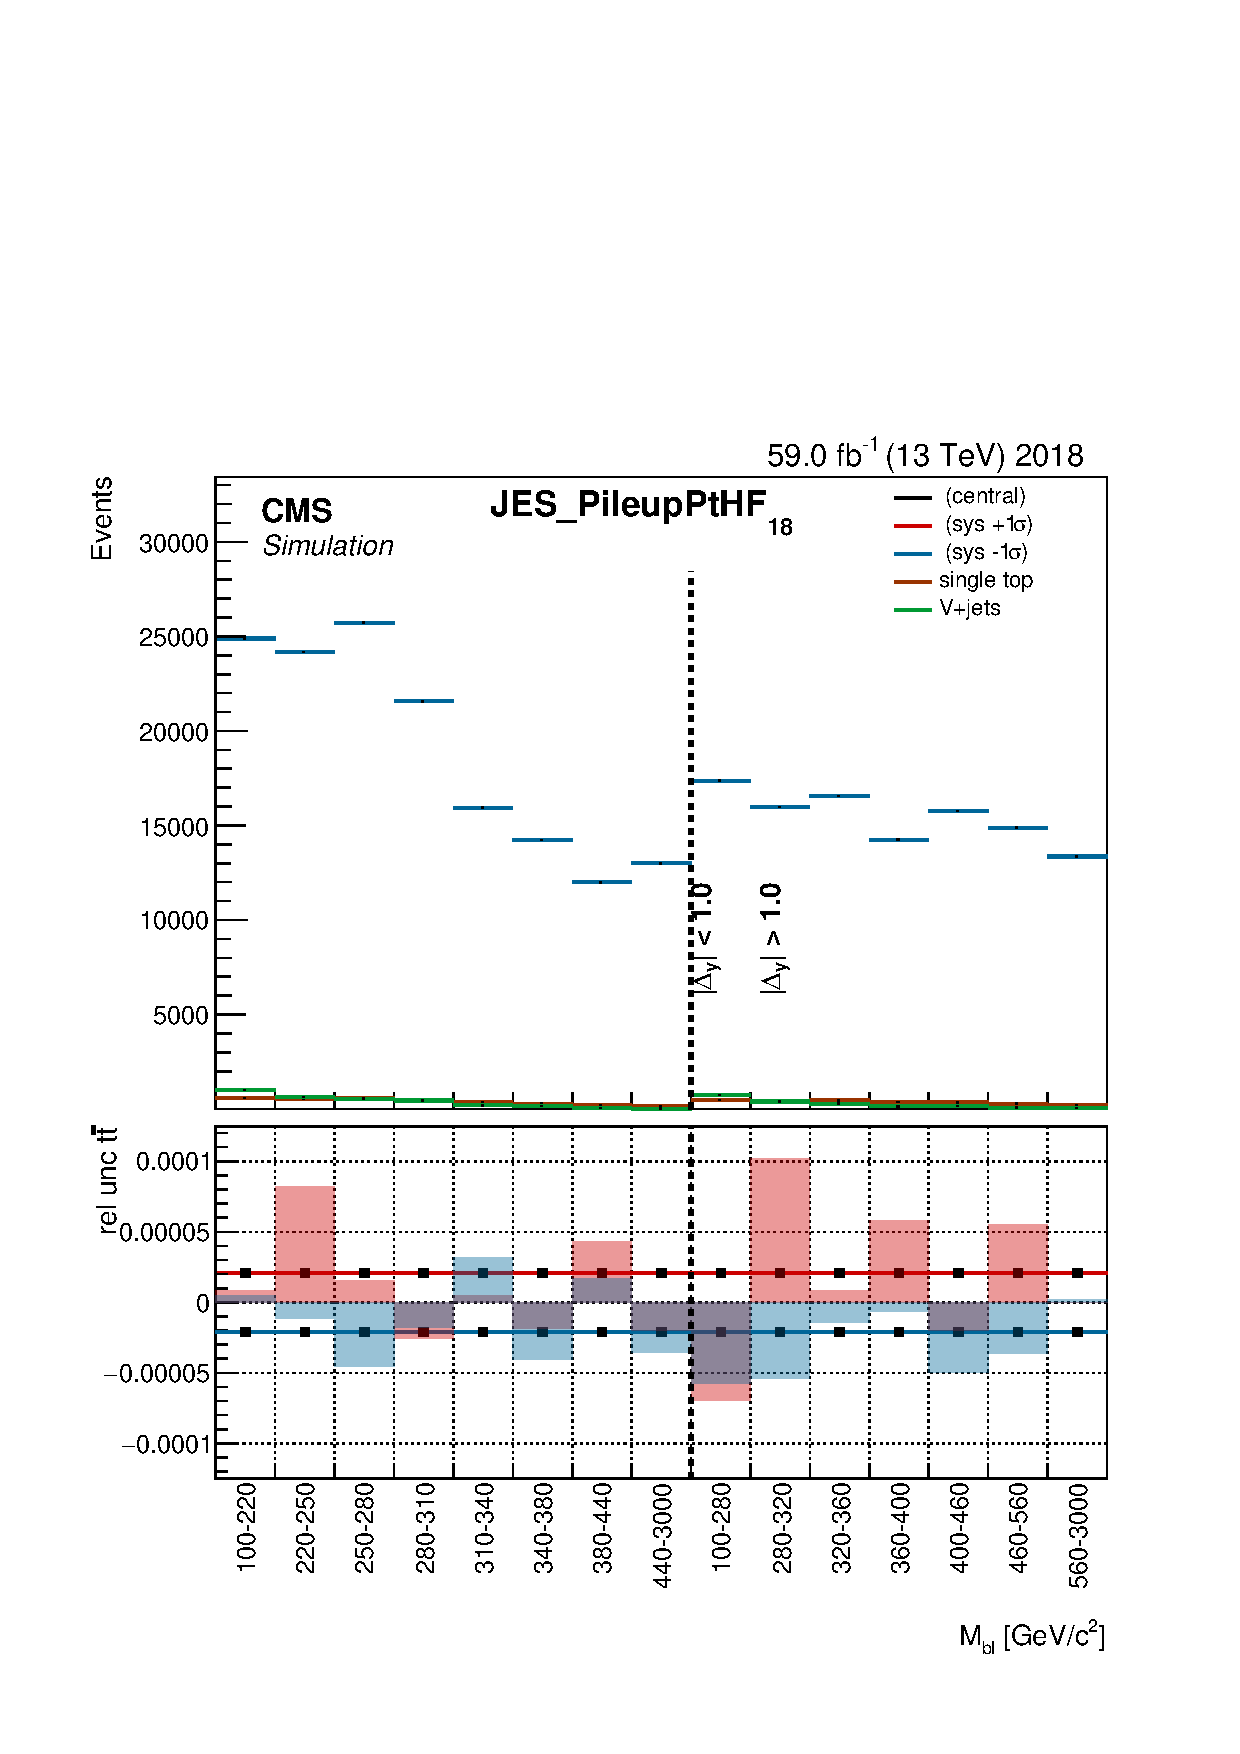
\includegraphics[width=.35\linewidth]{templates/JES_PileupPtHF_18}
\caption{JES\_PileupPtHF templates}
\label{fig:JES-PileupPtHF_template}
\end{figure}

\begin{figure} \centering
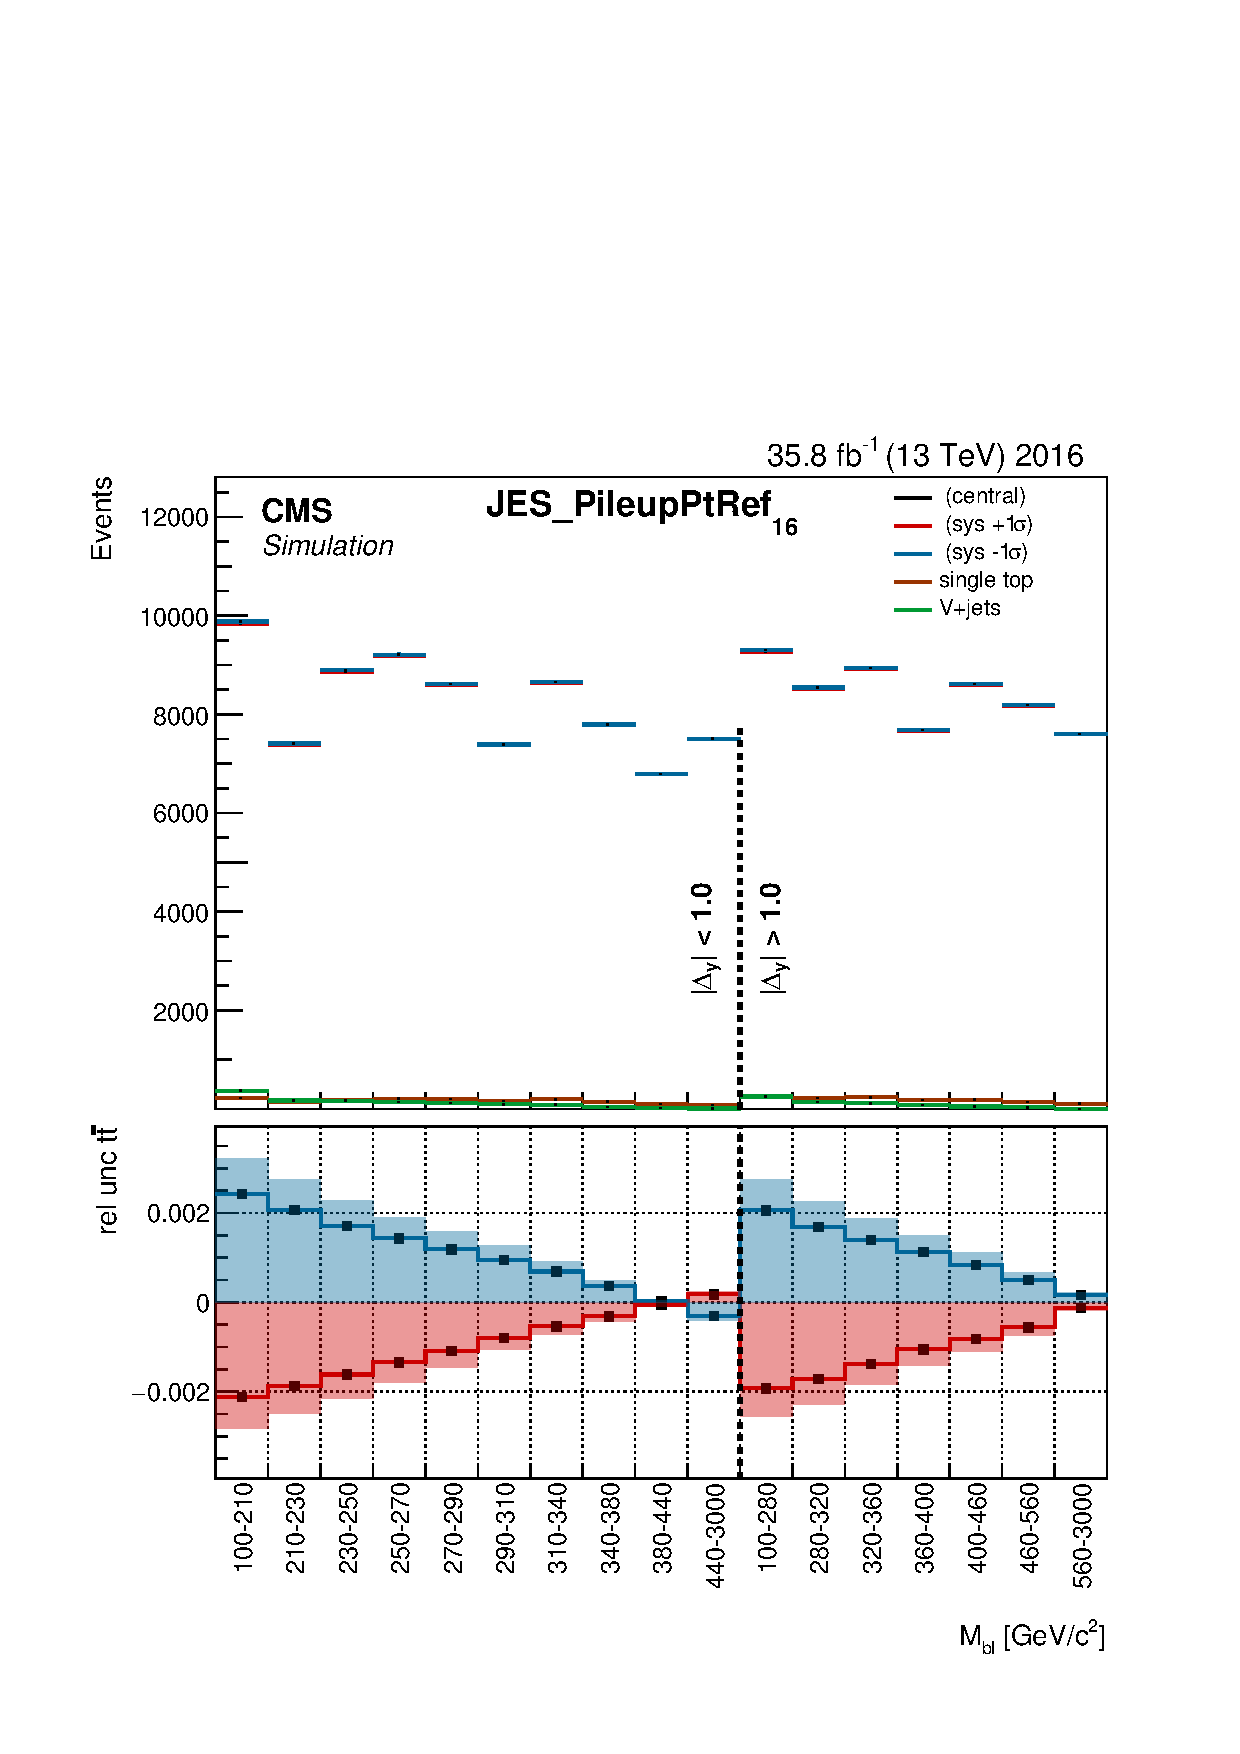
\includegraphics[width=.35\linewidth]{templates/JES_PileupPtRef_16}\hskip-.5cm
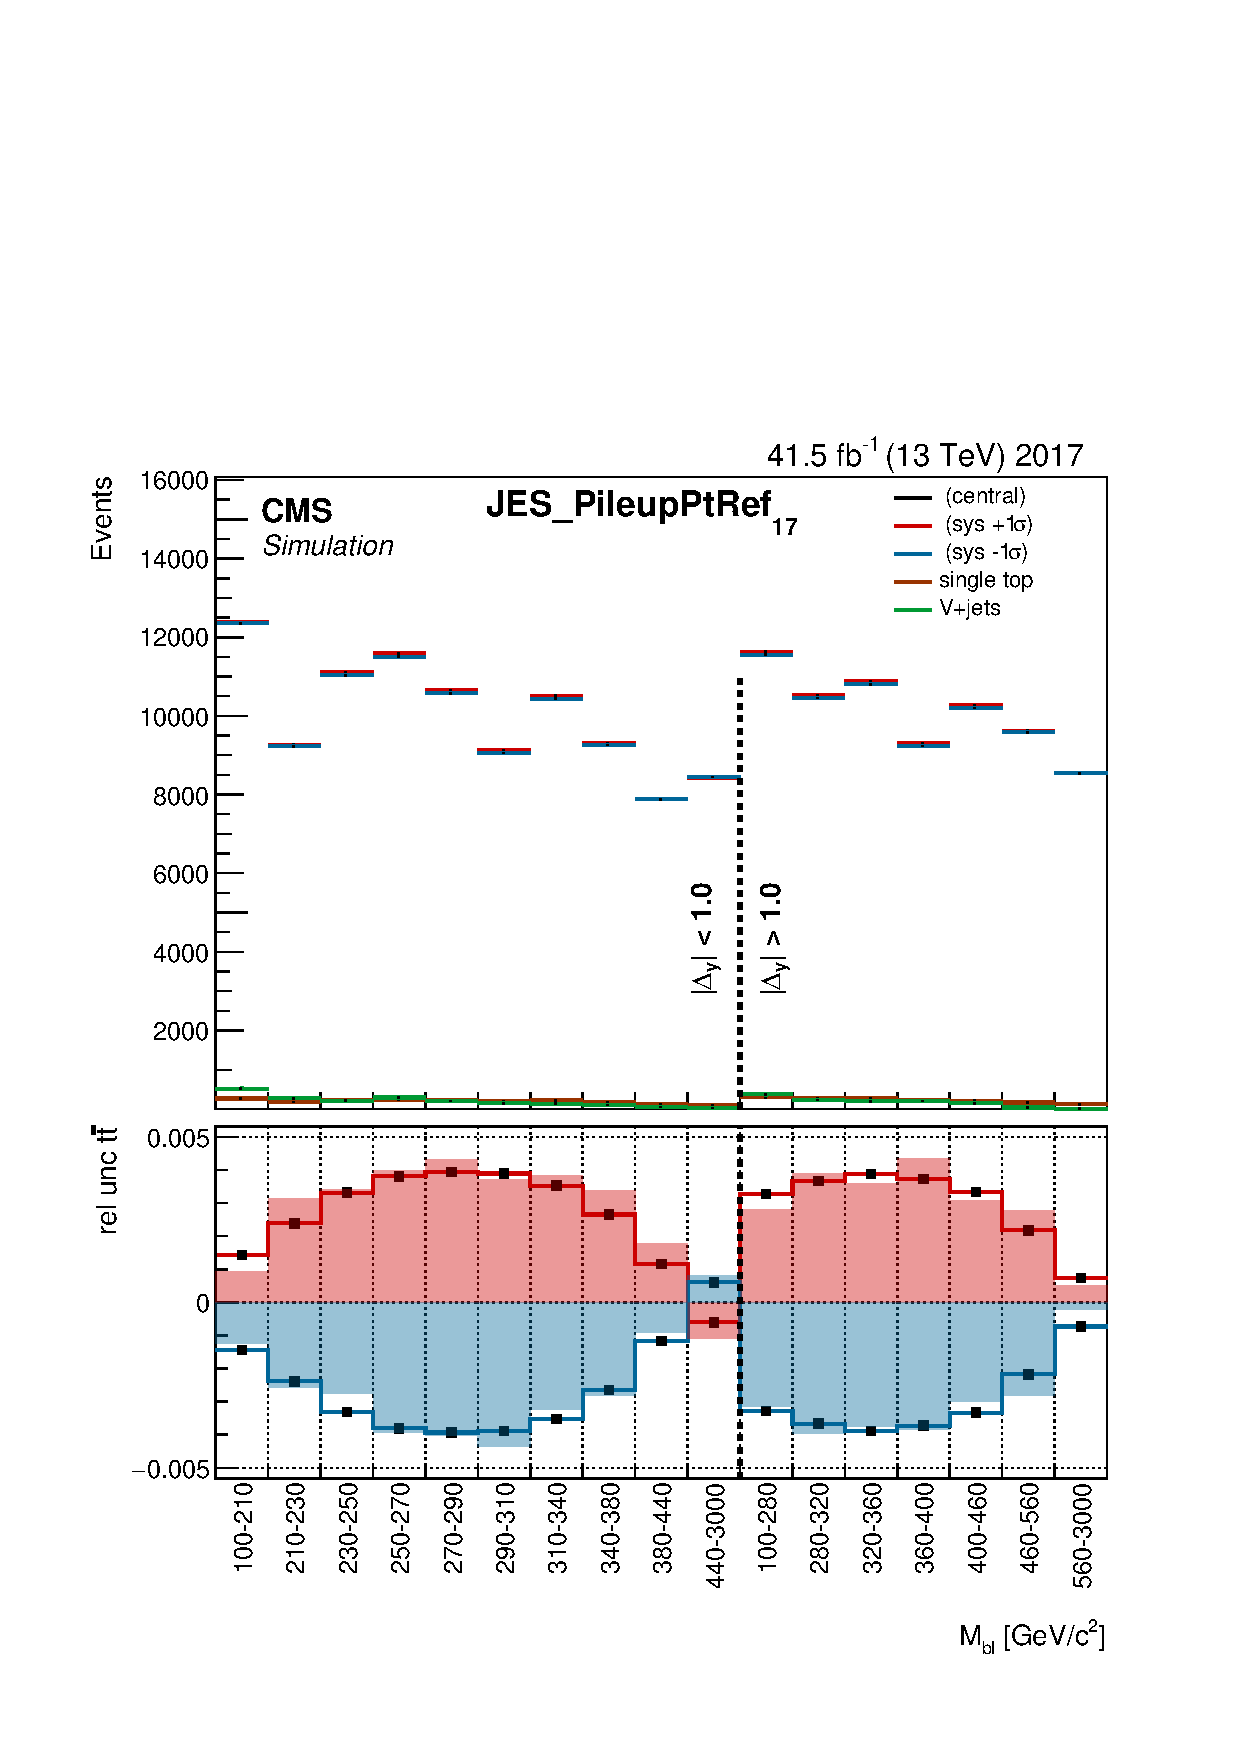
\includegraphics[width=.35\linewidth]{templates/JES_PileupPtRef_17}\hskip-.5cm
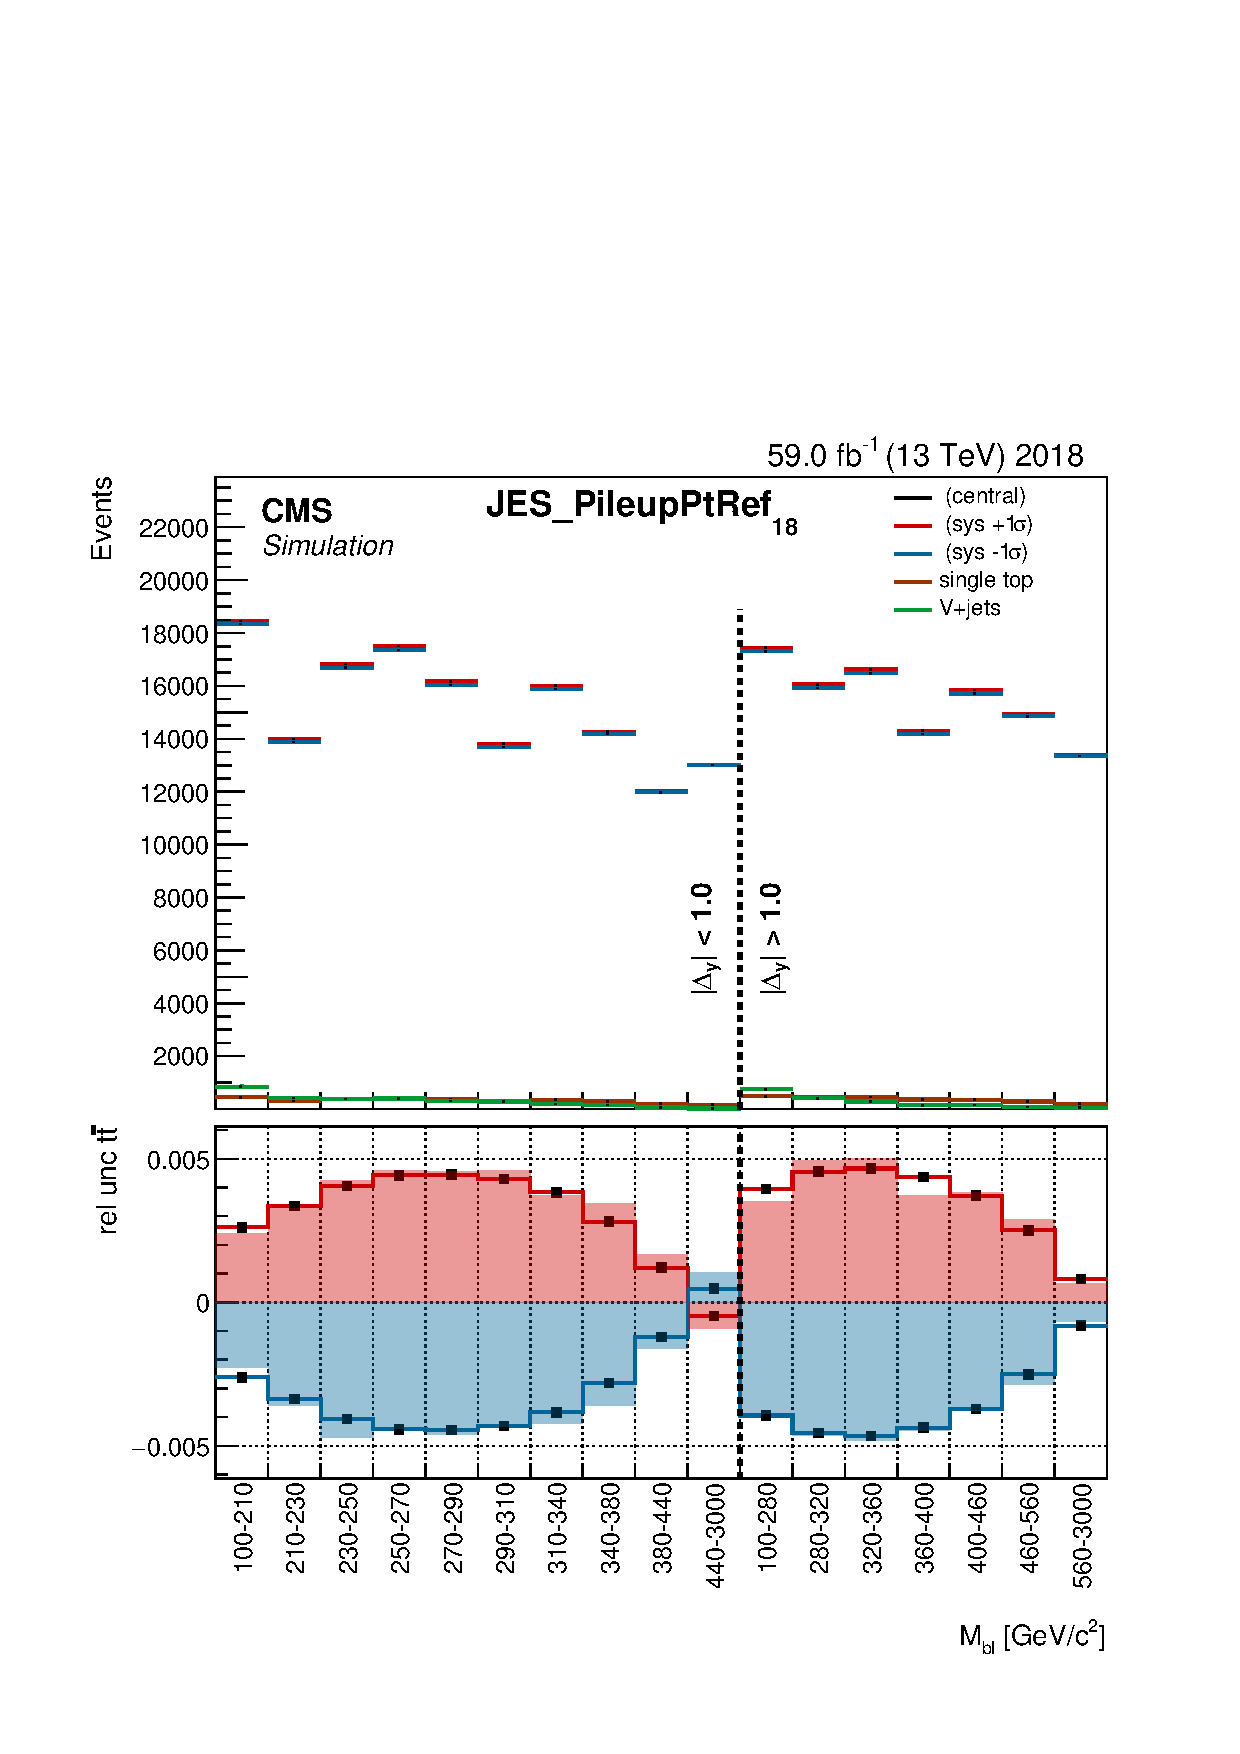
\includegraphics[width=.35\linewidth]{templates/JES_PileupPtRef_18}
\caption{JES\_PileupPtRef templates}
\label{fig:JES-PileupPtRef_template}
\end{figure}

\begin{figure} \centering
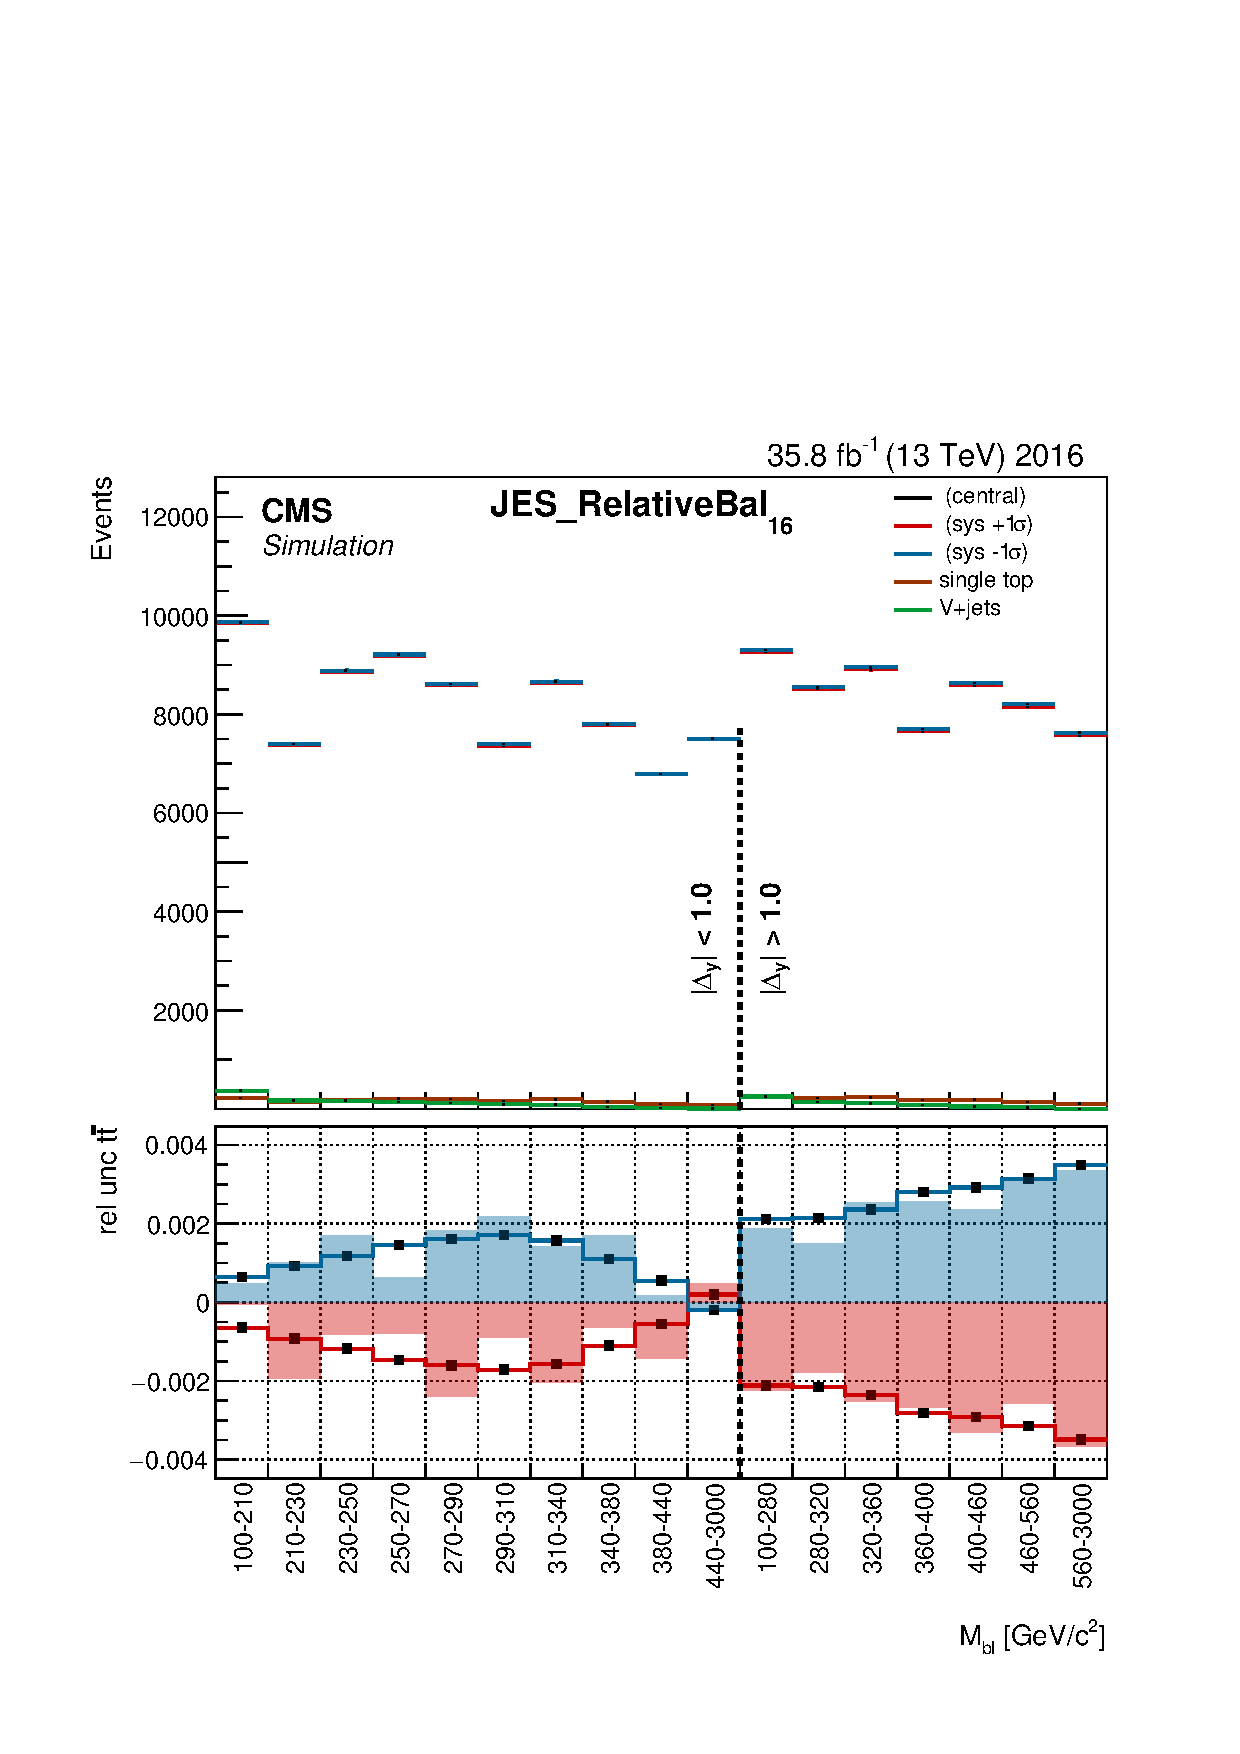
\includegraphics[width=.35\linewidth]{templates/JES_RelativeBal_16}\hskip-.5cm
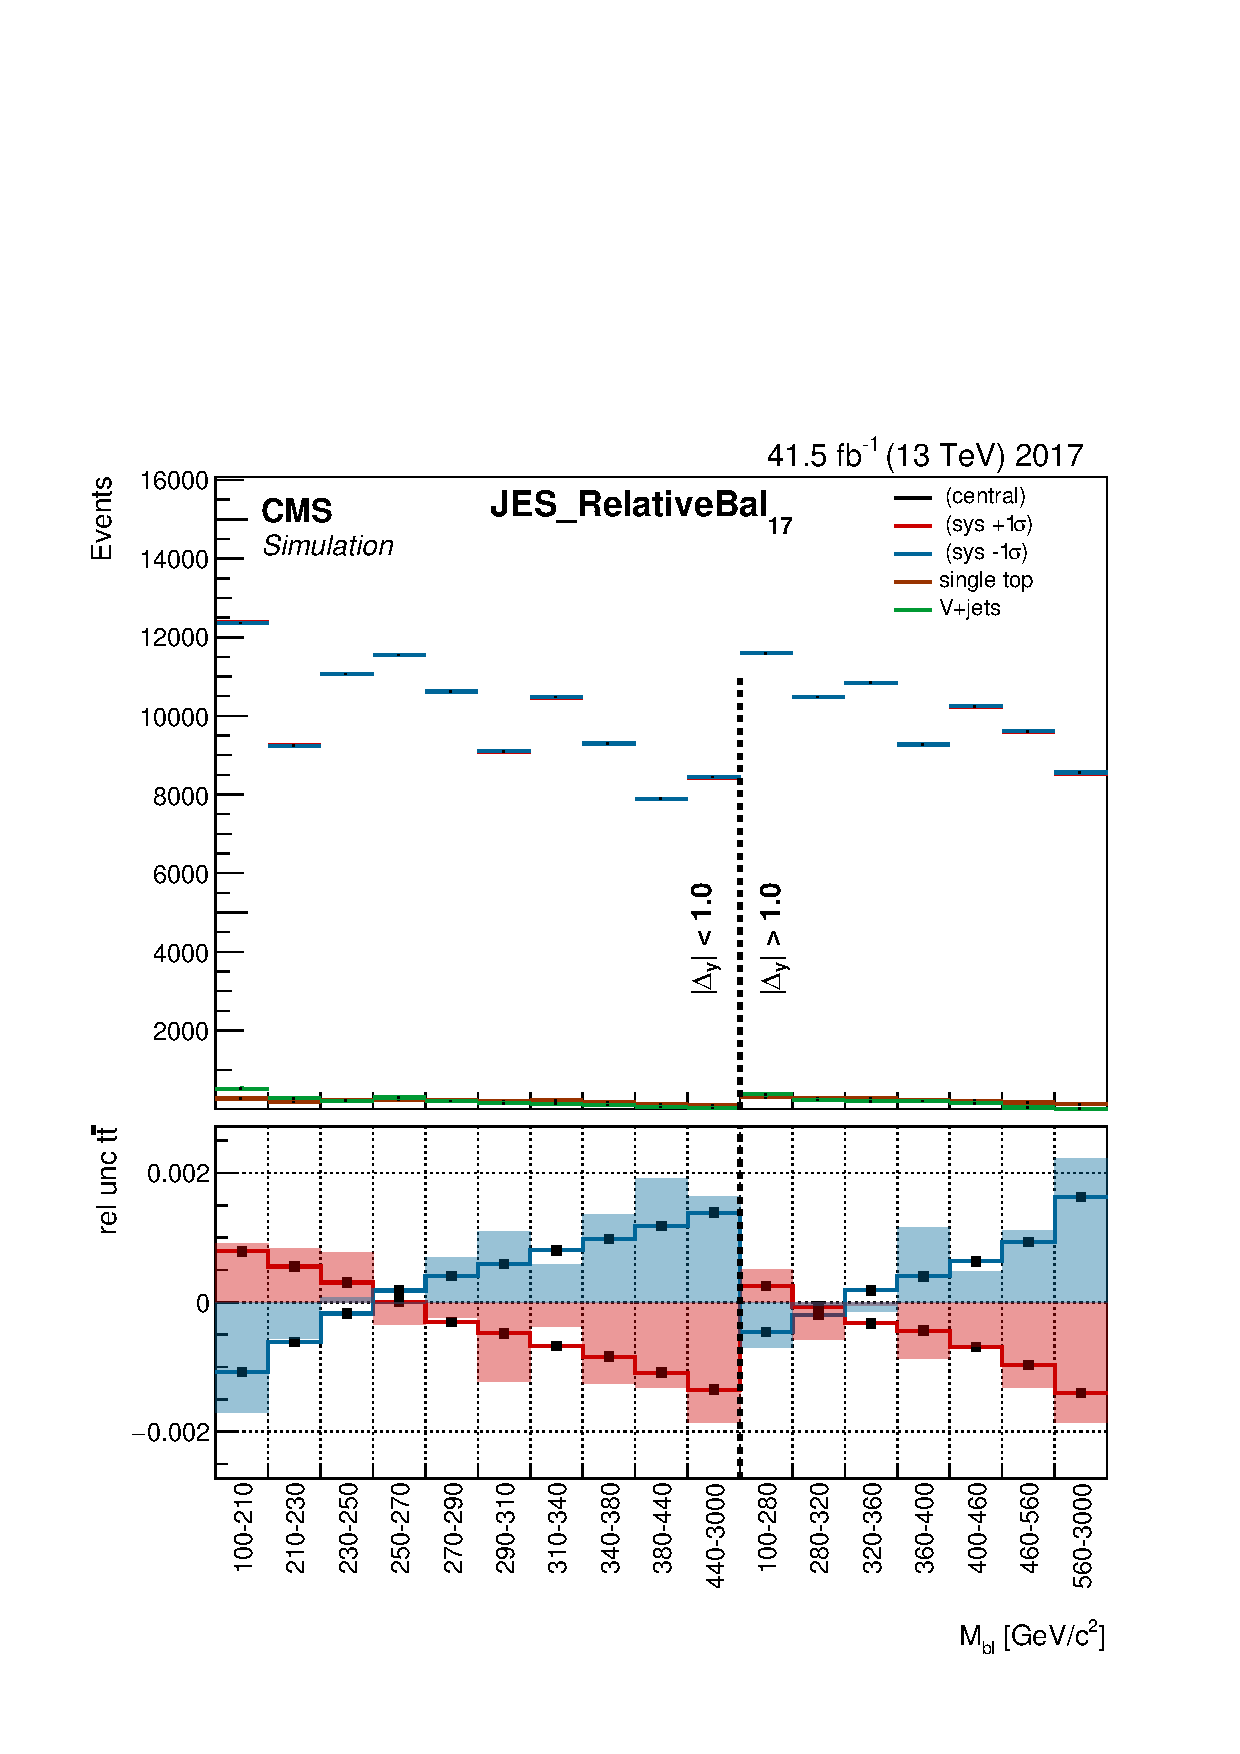
\includegraphics[width=.35\linewidth]{templates/JES_RelativeBal_17}\hskip-.5cm
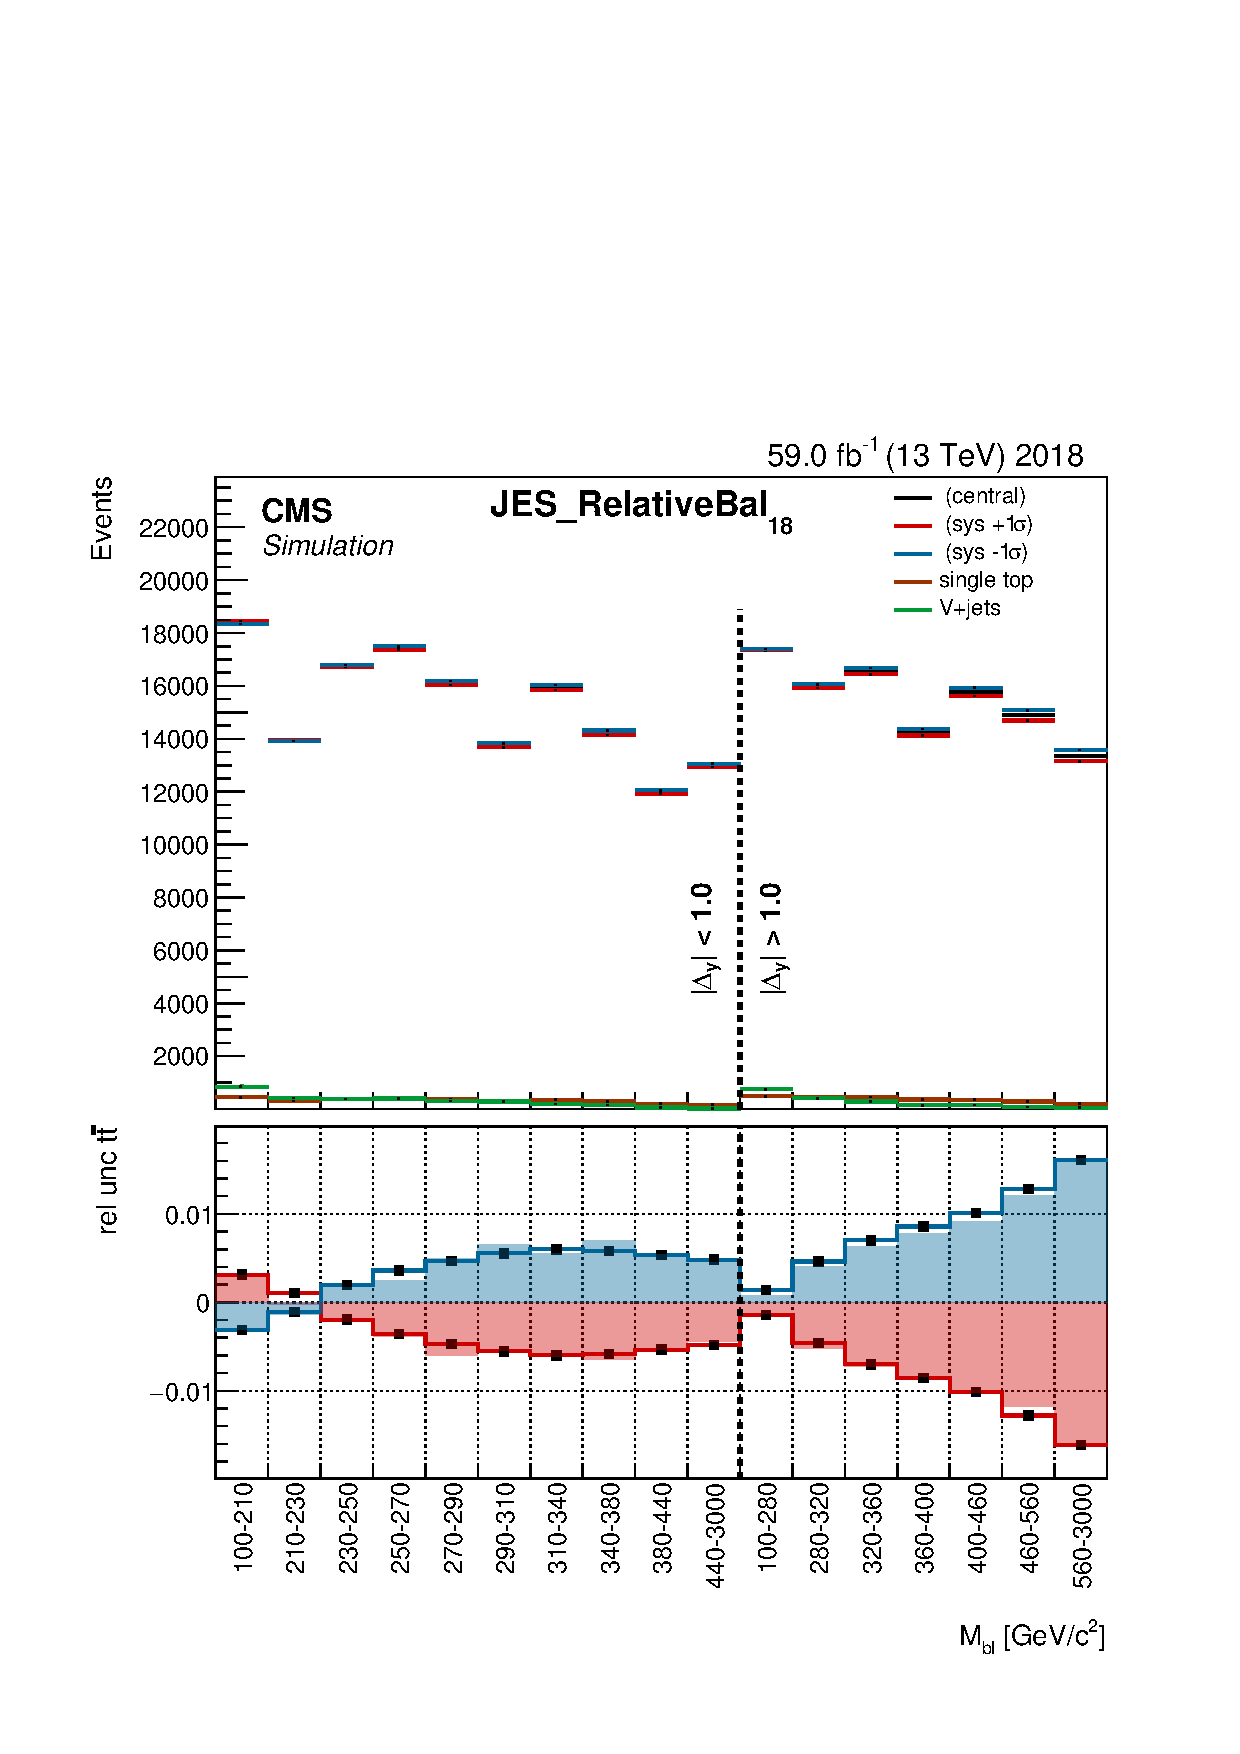
\includegraphics[width=.35\linewidth]{templates/JES_RelativeBal_18}
\caption{JES\_RelativeBal templates}
\label{fig:JES-RelativeBal_template}
\end{figure}

\begin{figure} \centering
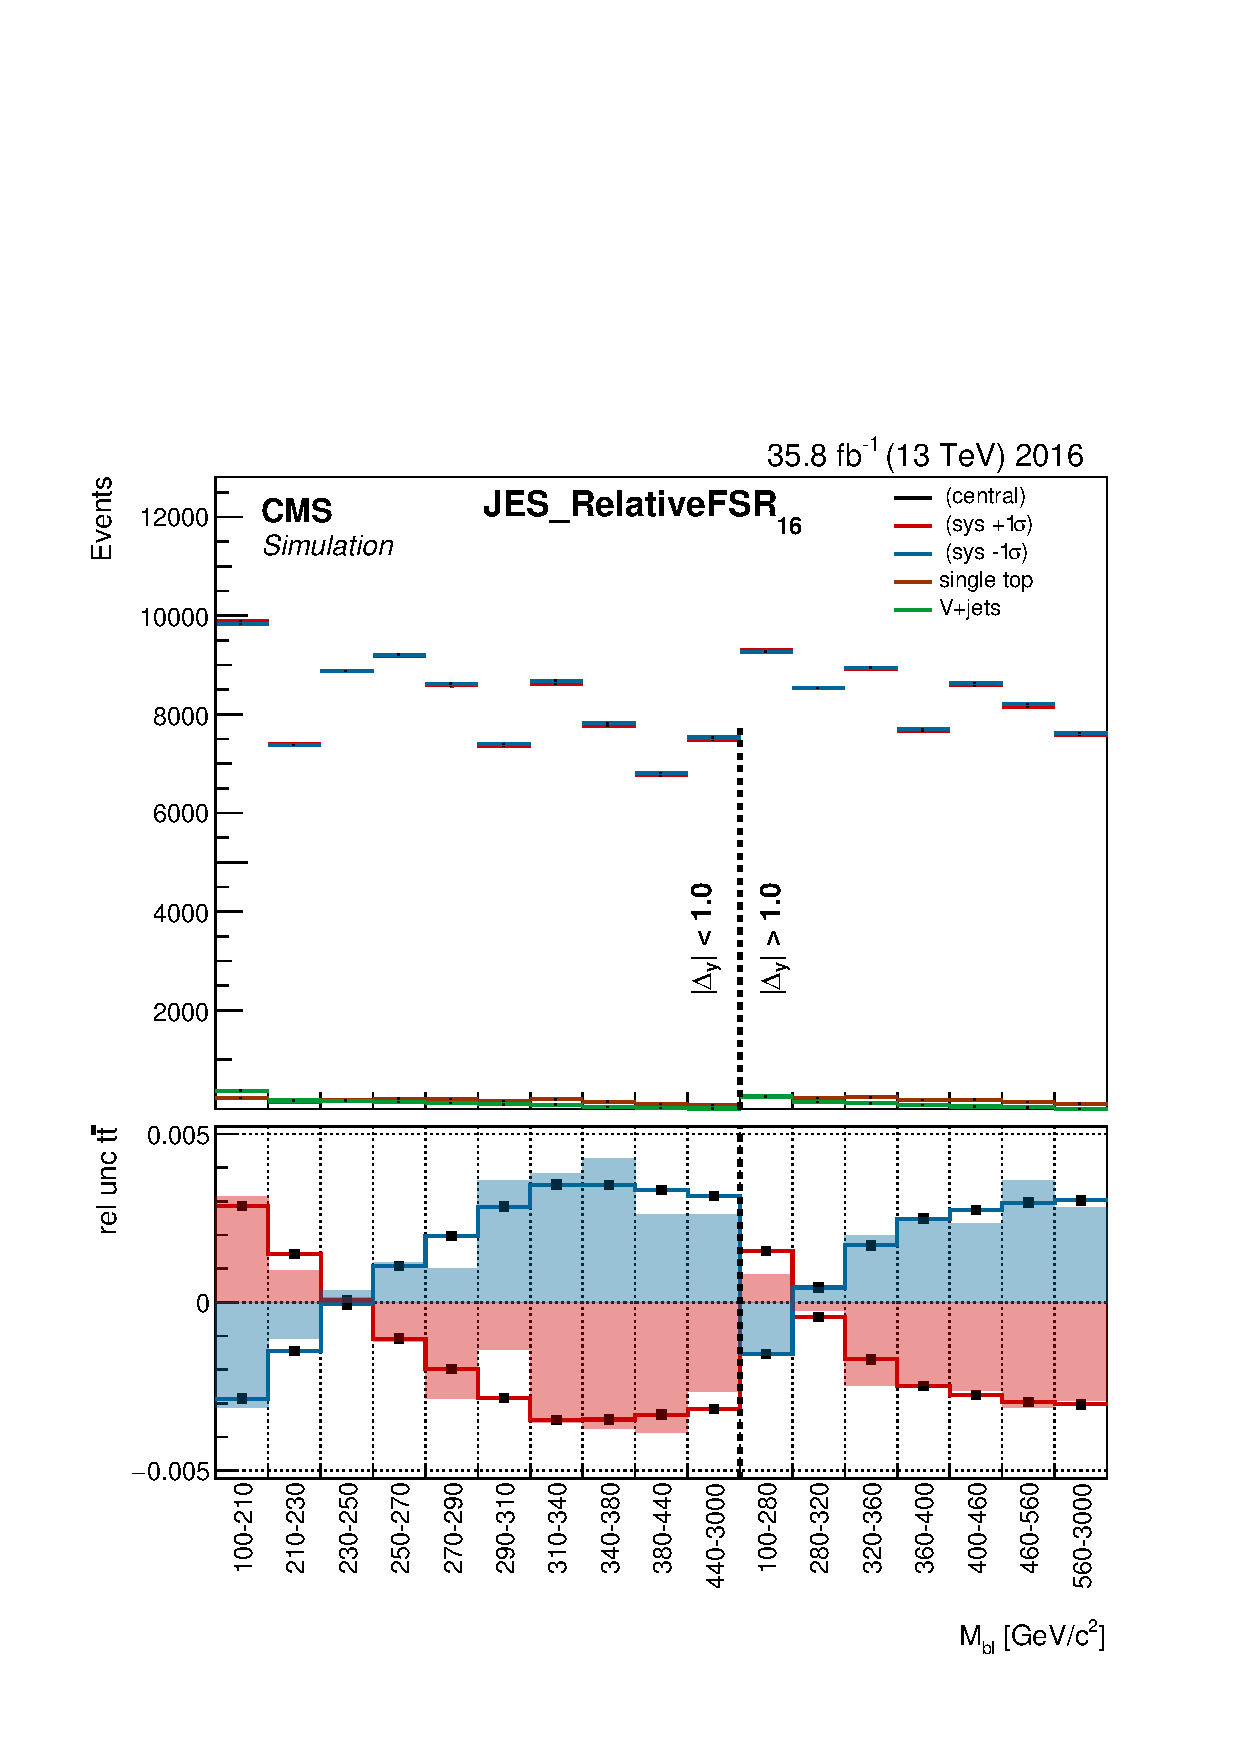
\includegraphics[width=.35\linewidth]{templates/JES_RelativeFSR_16}\hskip-.5cm
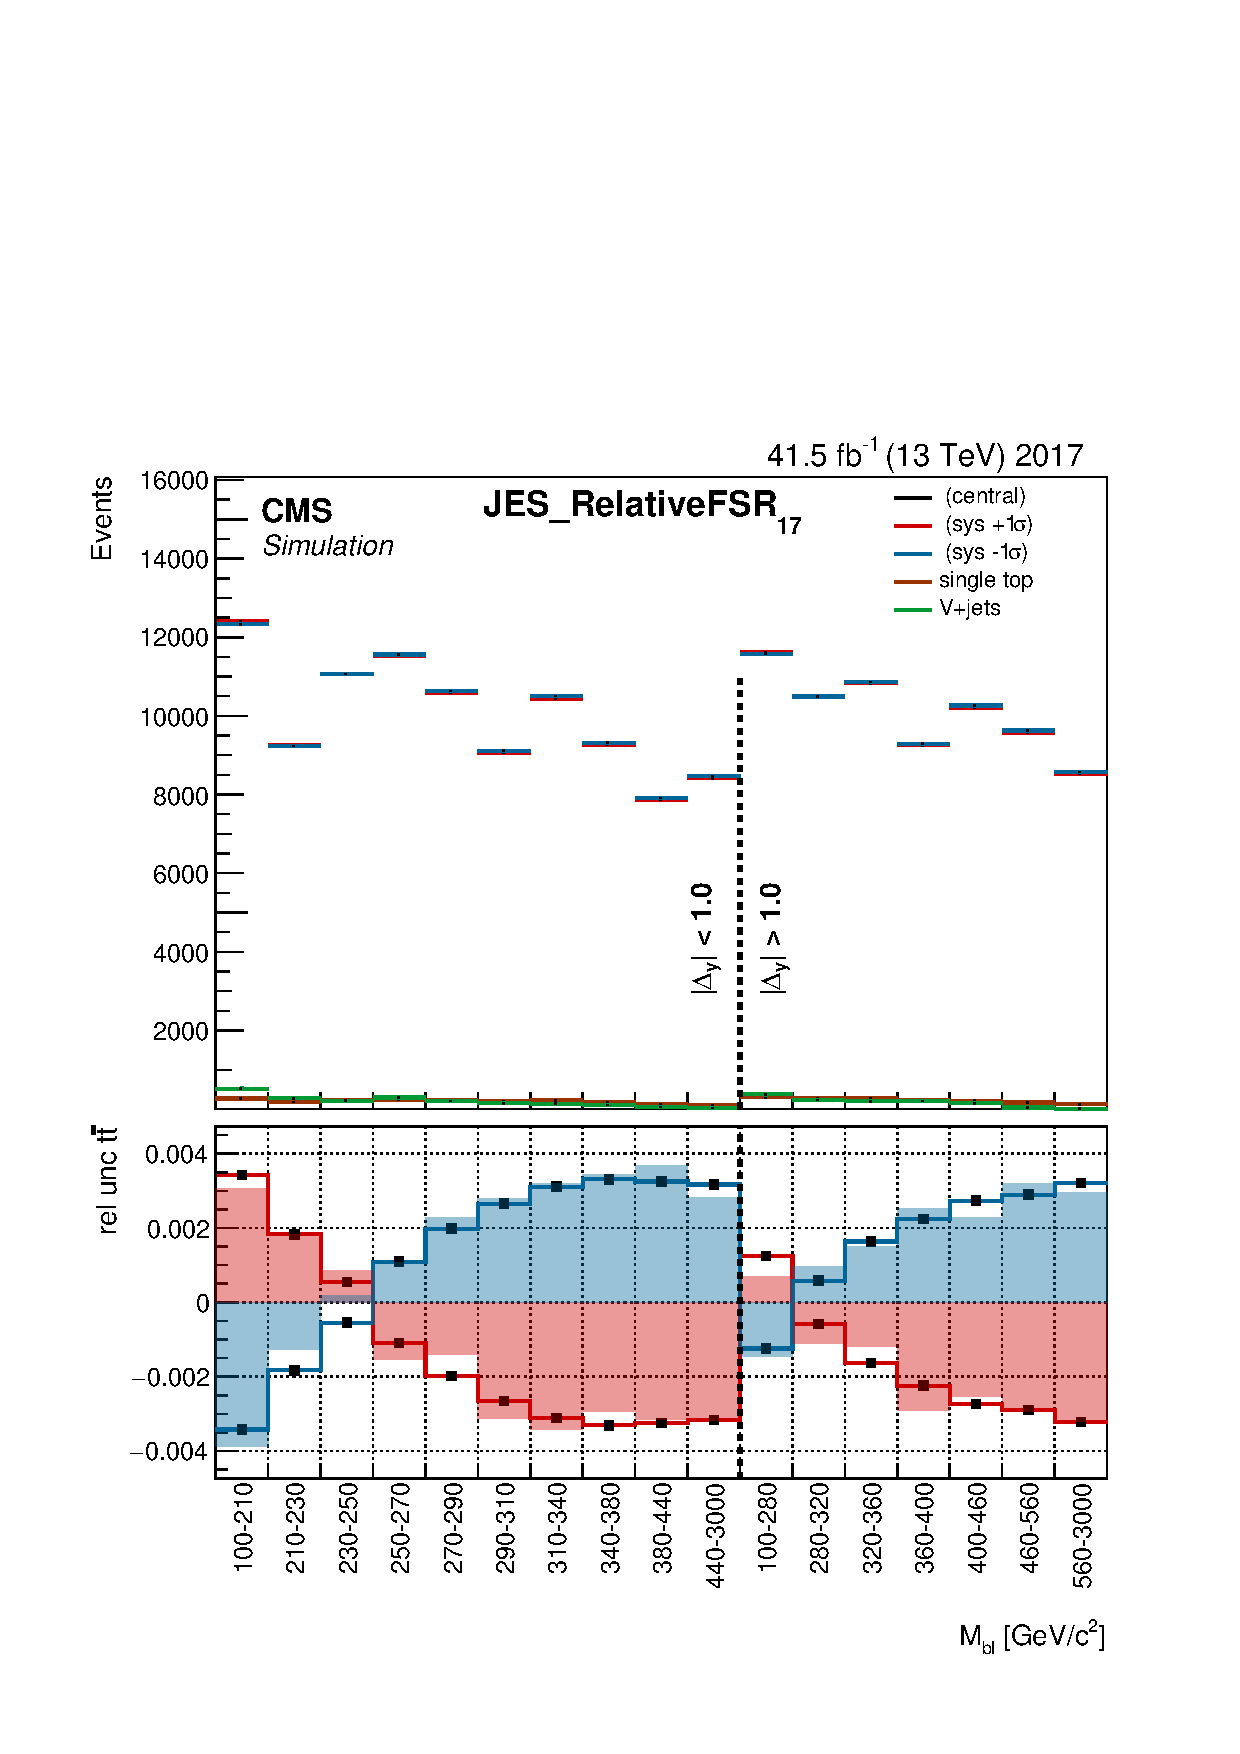
\includegraphics[width=.35\linewidth]{templates/JES_RelativeFSR_17}\hskip-.5cm
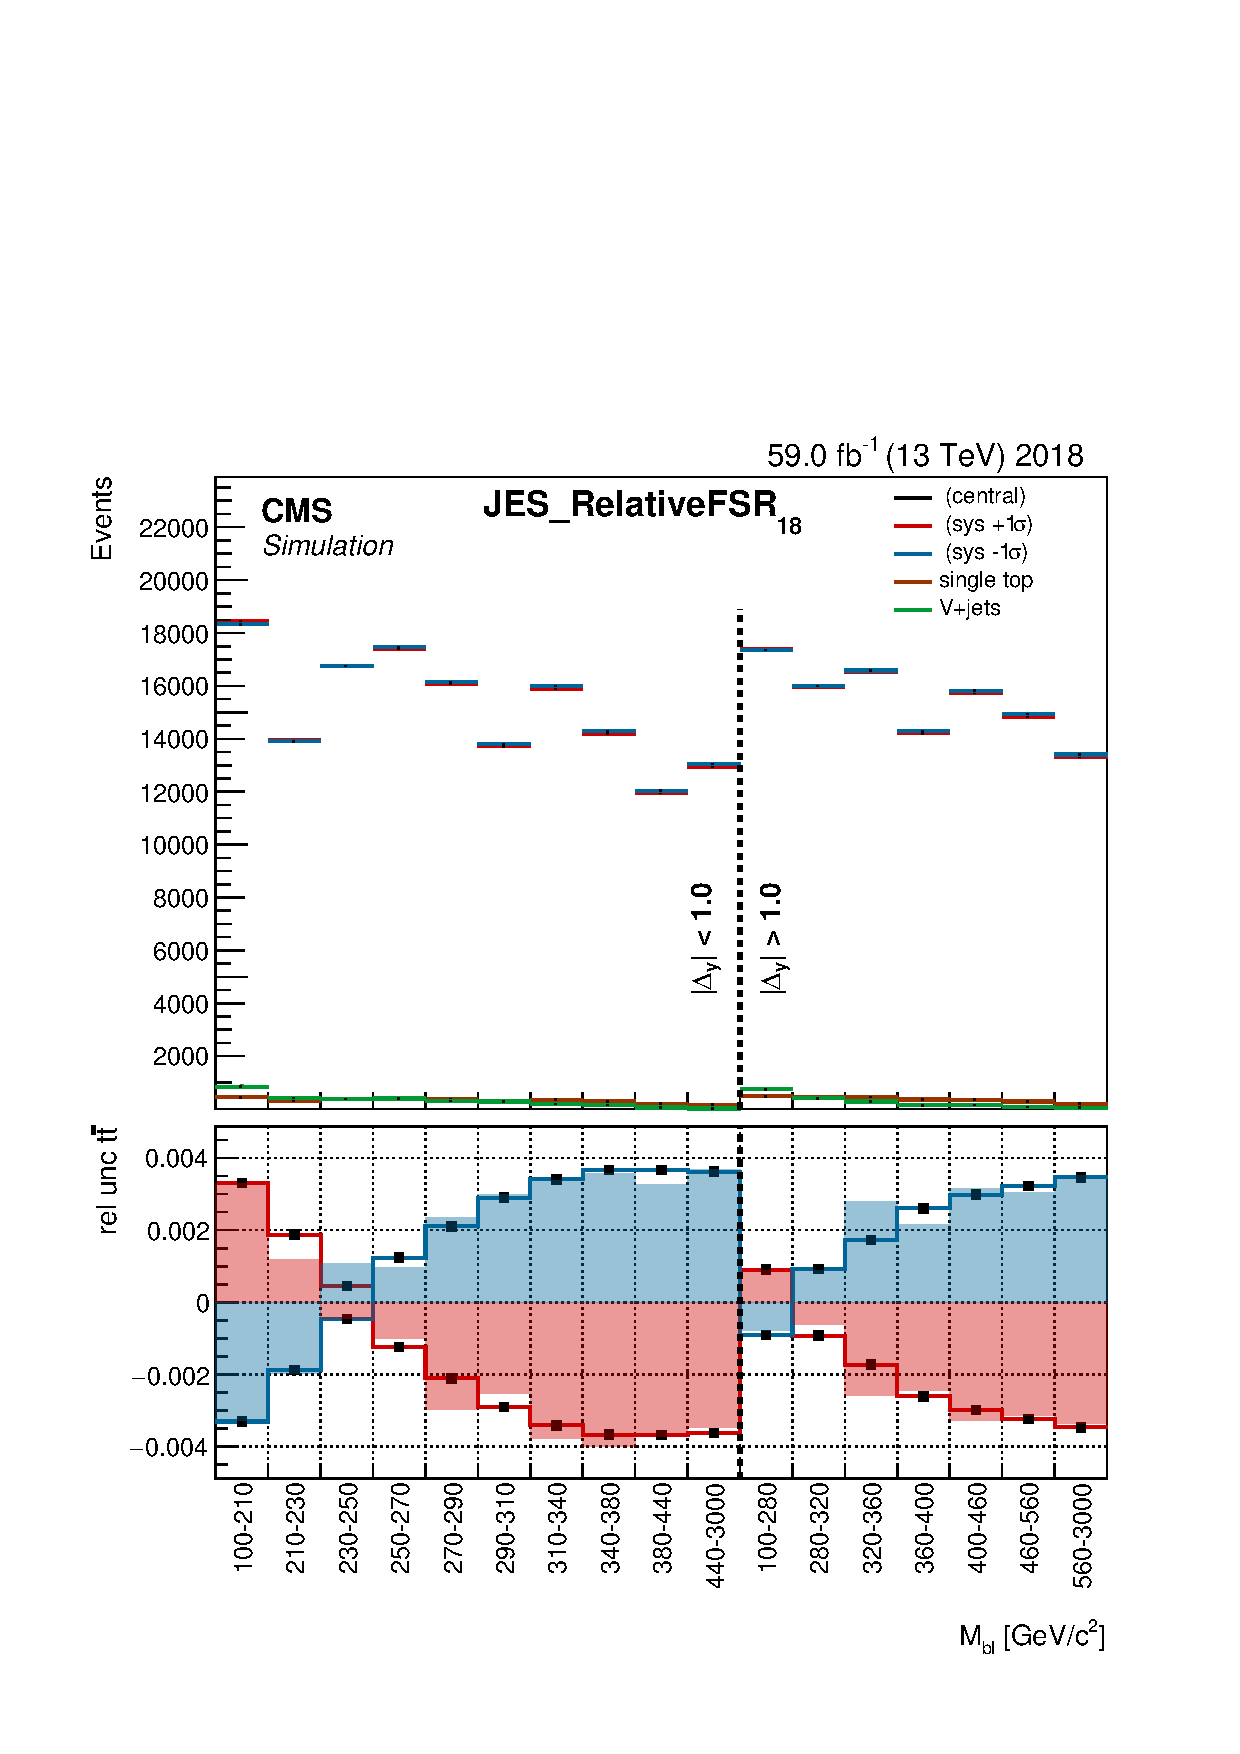
\includegraphics[width=.35\linewidth]{templates/JES_RelativeFSR_18}
\caption{JES\_RelativeFSR templates}
\label{fig:JES-RelativeFSR_template}
\end{figure}

\begin{figure} \centering
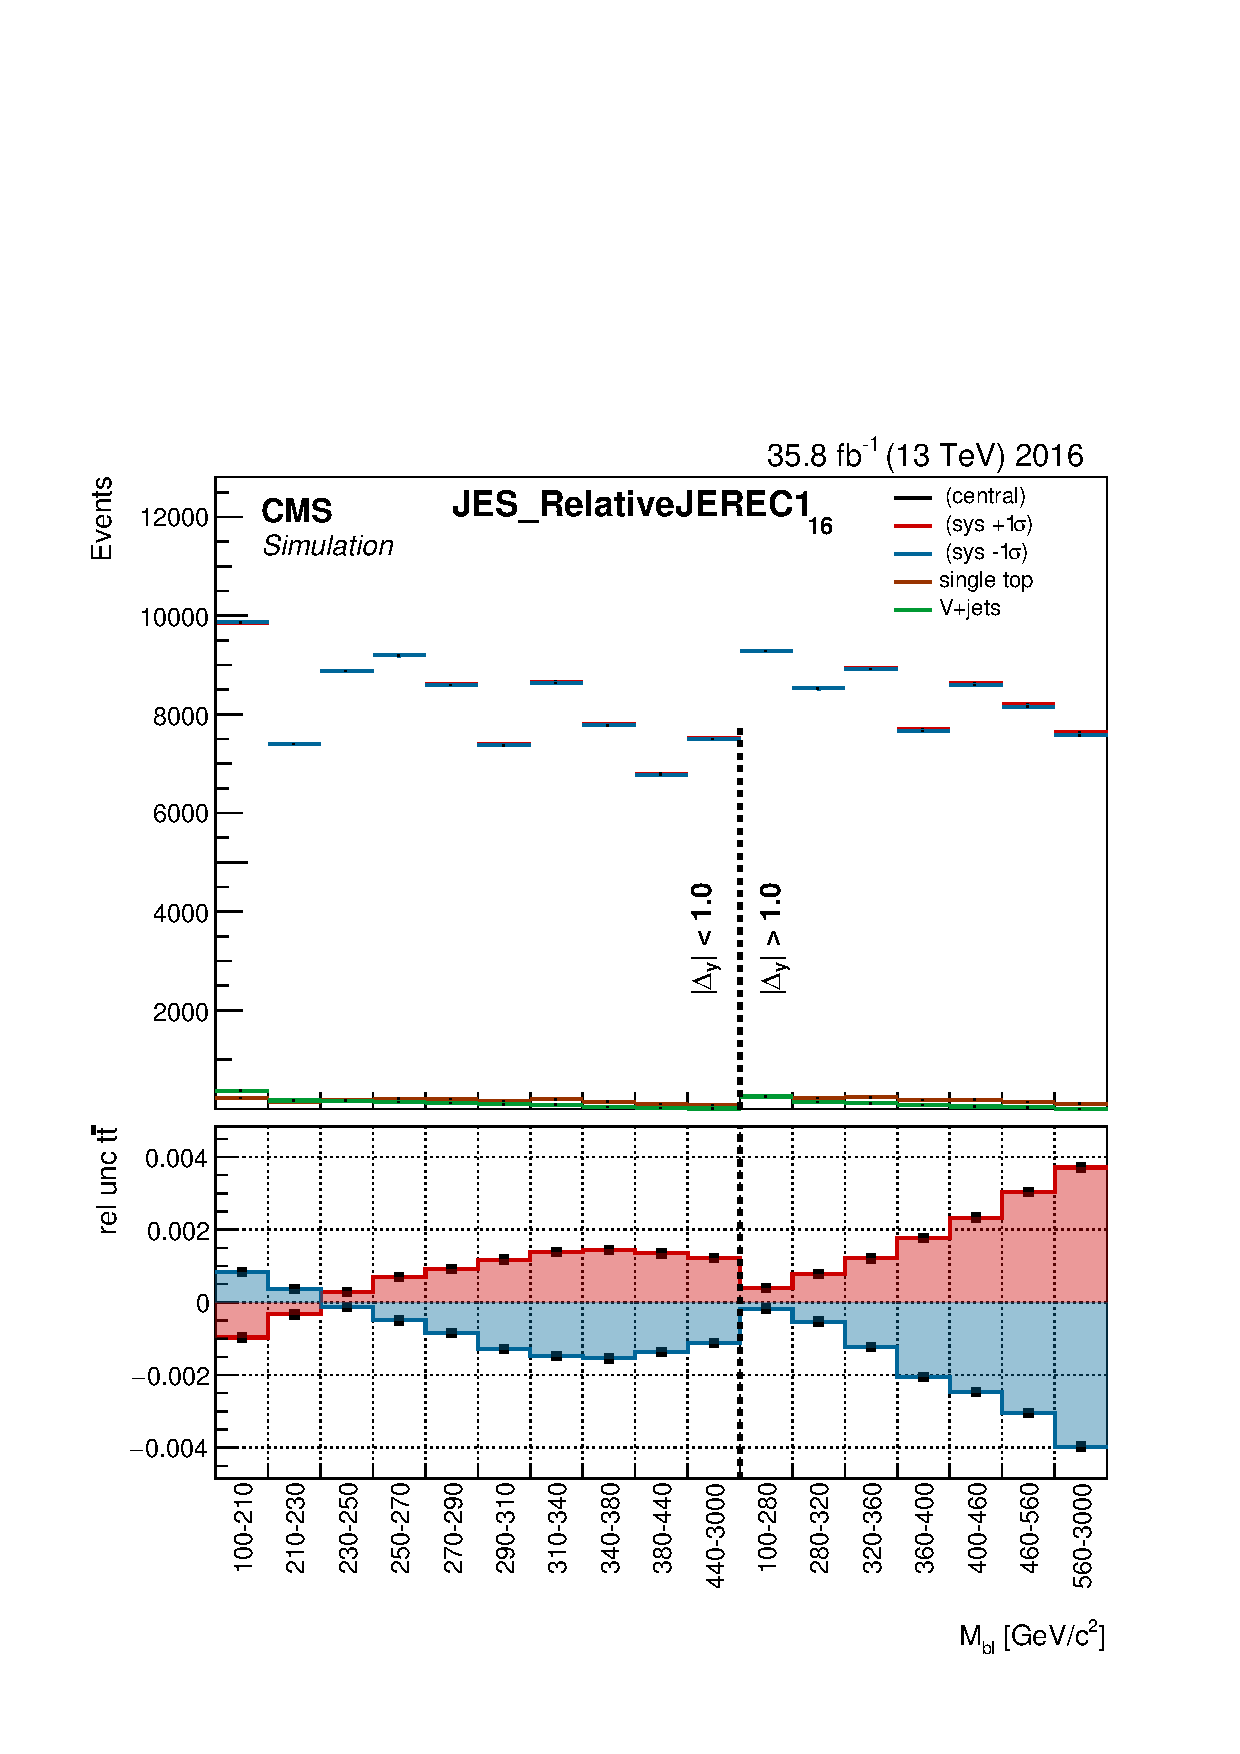
\includegraphics[width=.35\linewidth]{templates/JES_RelativeJEREC1_16}\hskip-.5cm
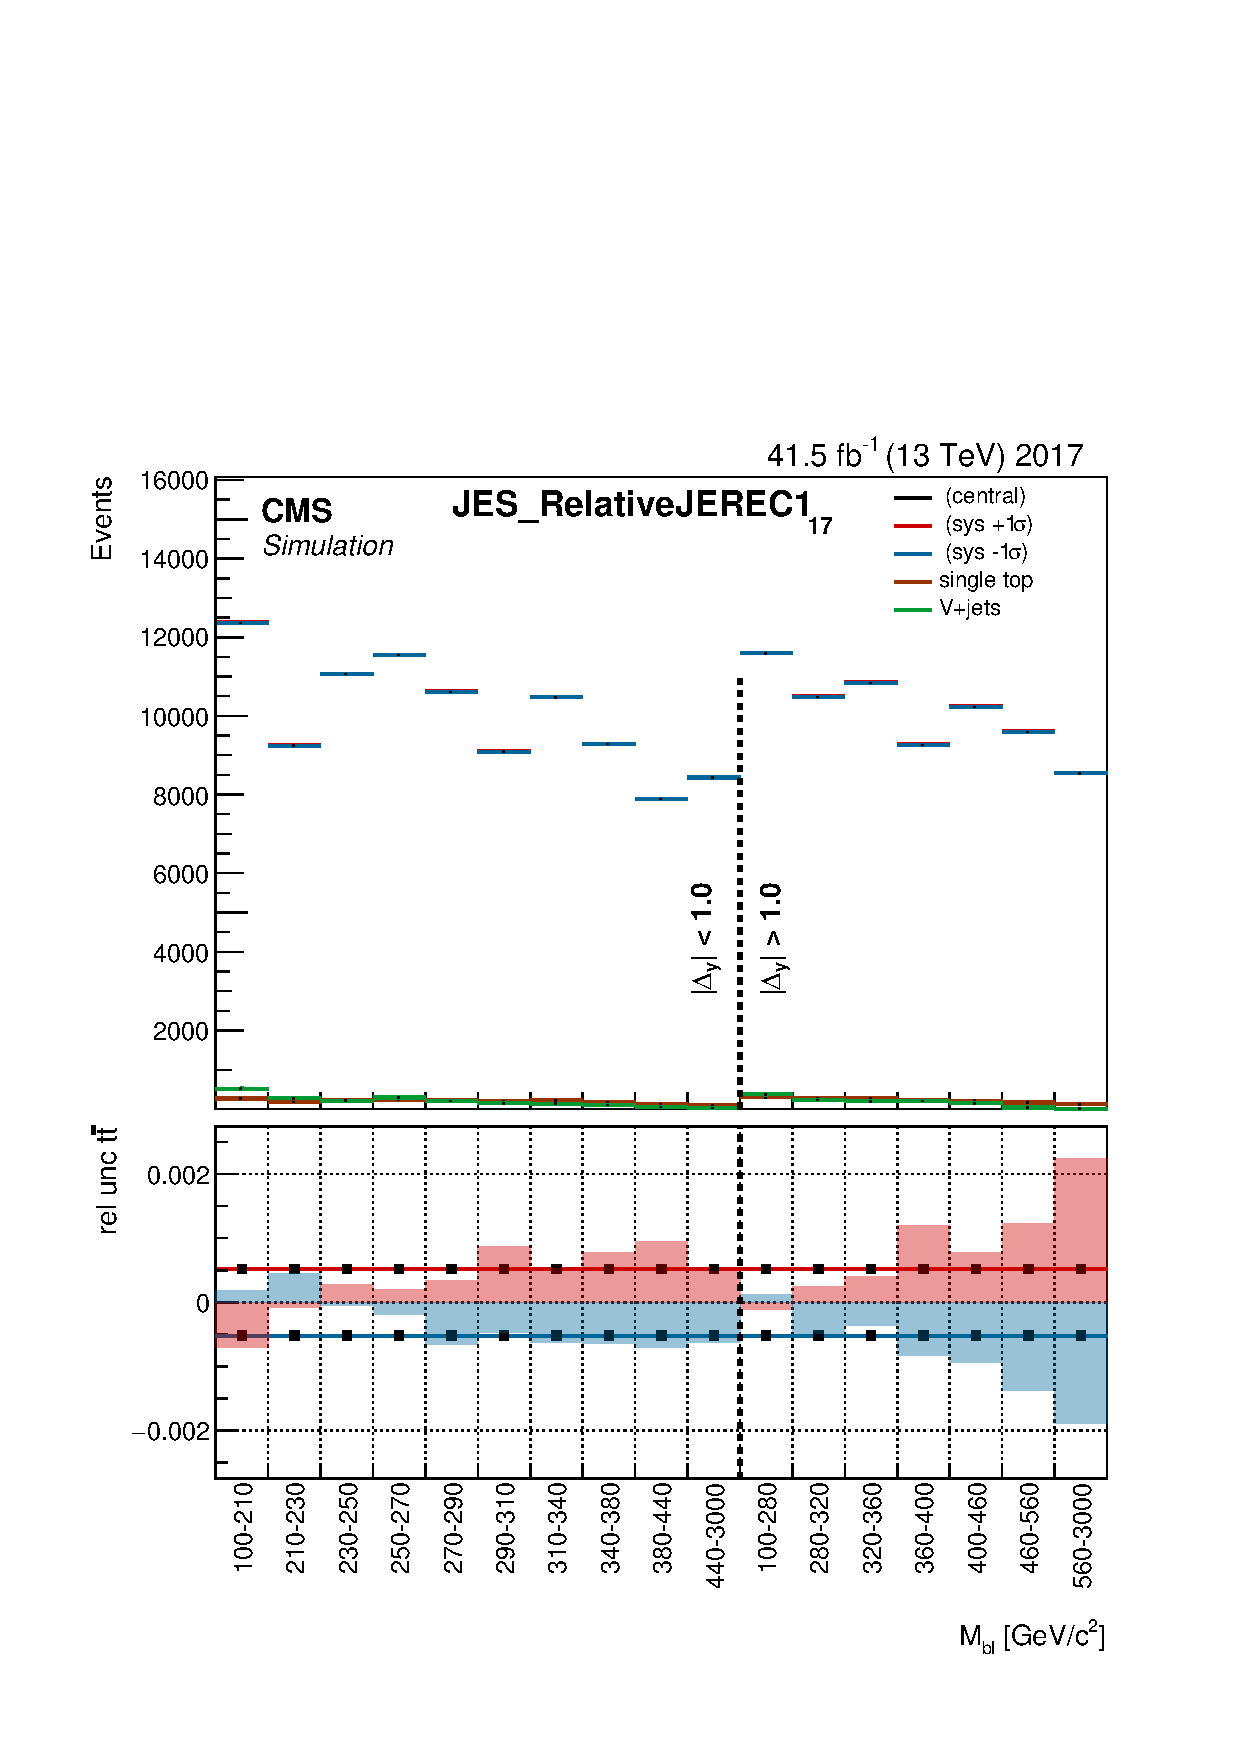
\includegraphics[width=.35\linewidth]{templates/JES_RelativeJEREC1_17}\hskip-.5cm
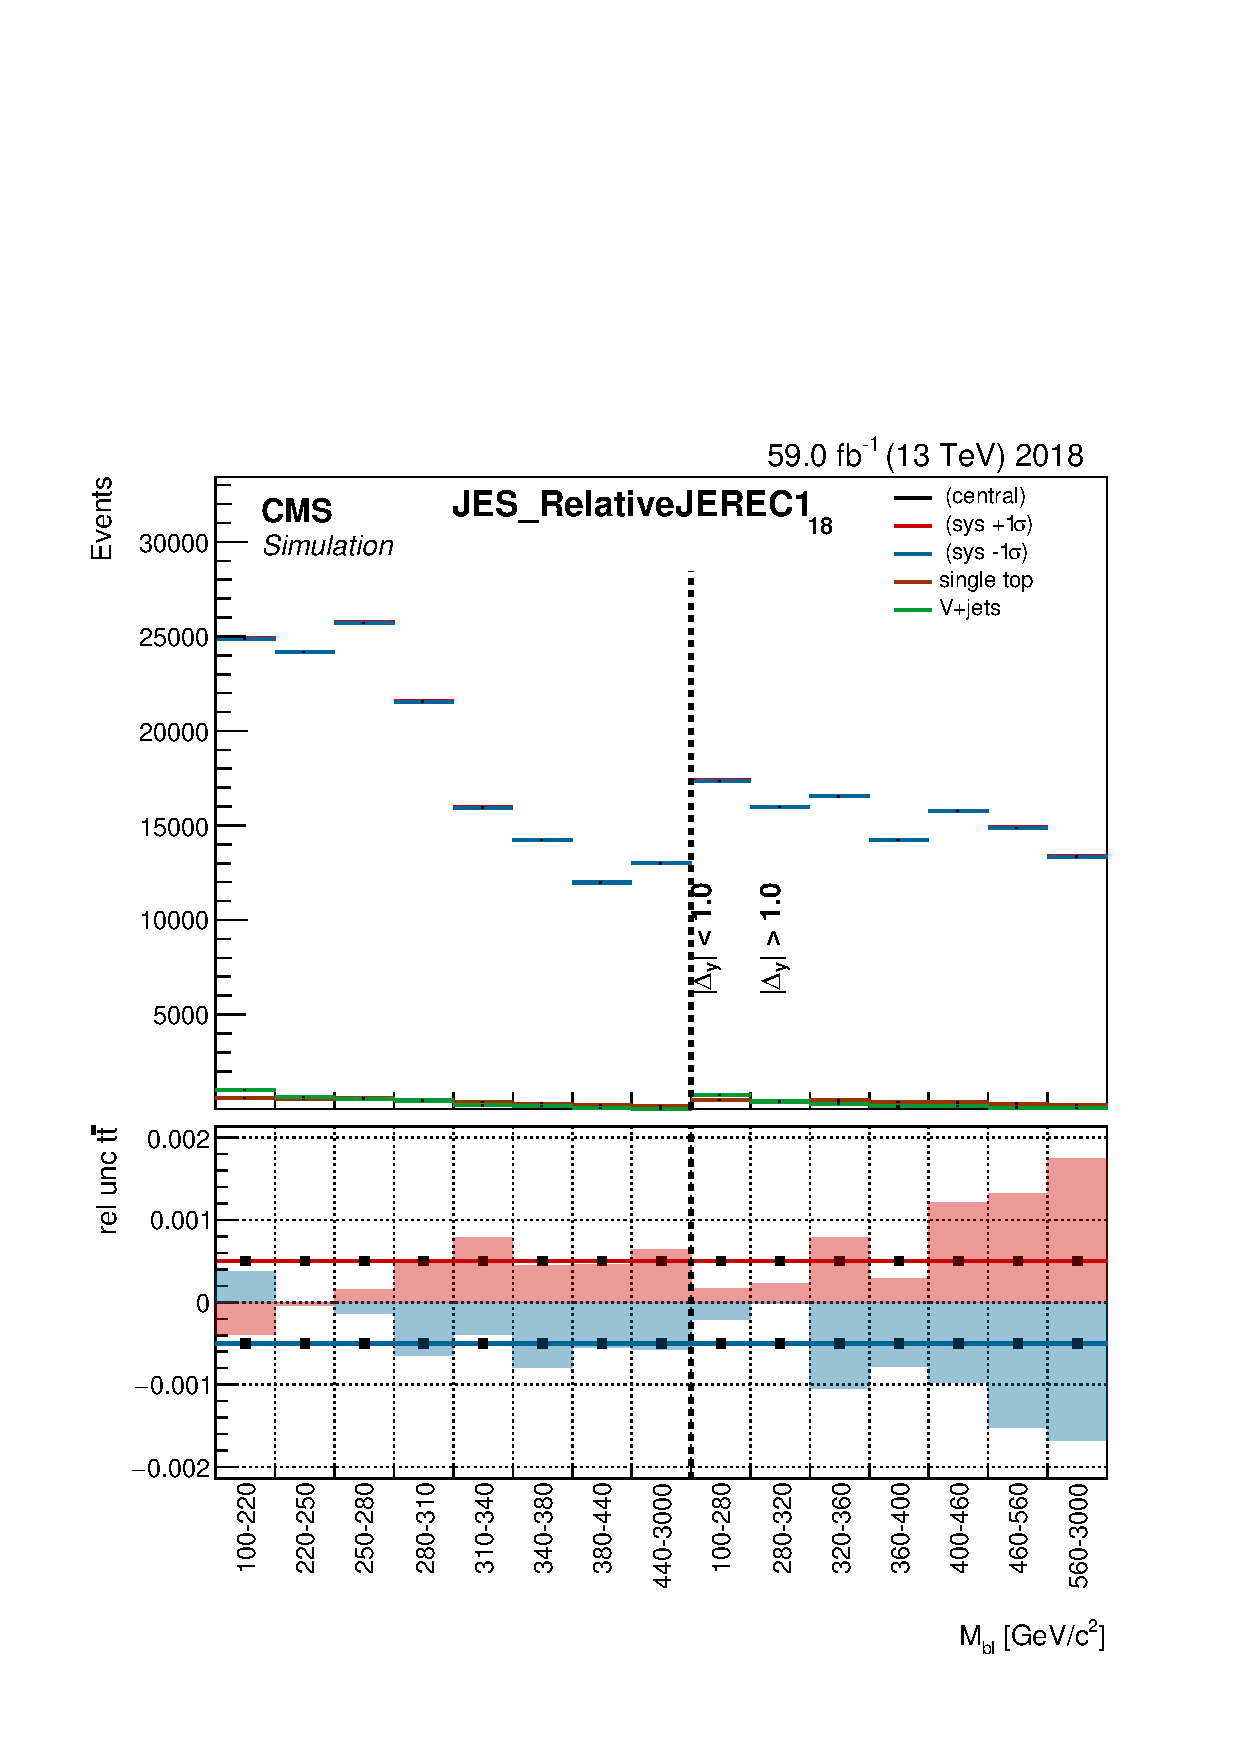
\includegraphics[width=.35\linewidth]{templates/JES_RelativeJEREC1_18}
\caption{JES\_RelativeJEREC1 templates}
\label{fig:JES-RelativeJEREC1_template}
\end{figure}

\begin{figure} \centering
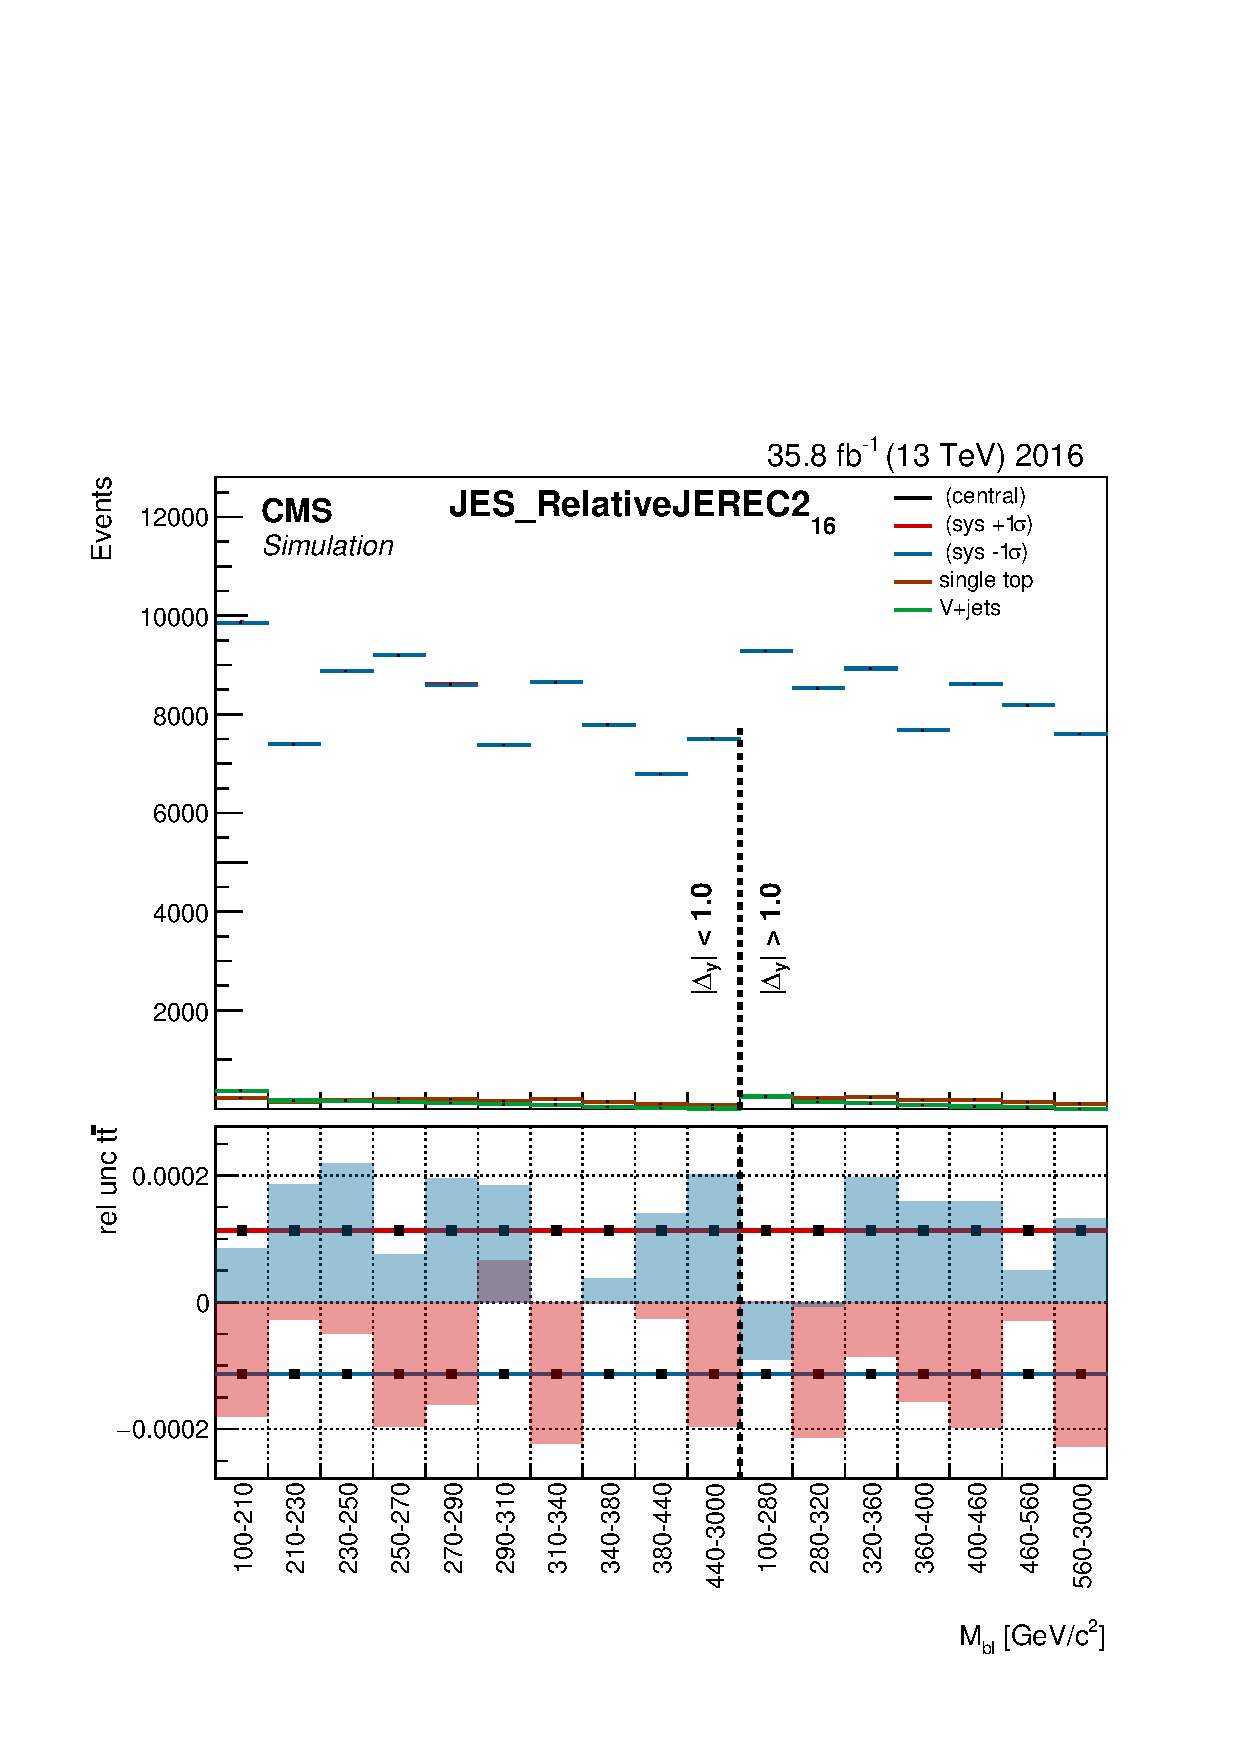
\includegraphics[width=.35\linewidth]{templates/JES_RelativeJEREC2_16}\hskip-.5cm
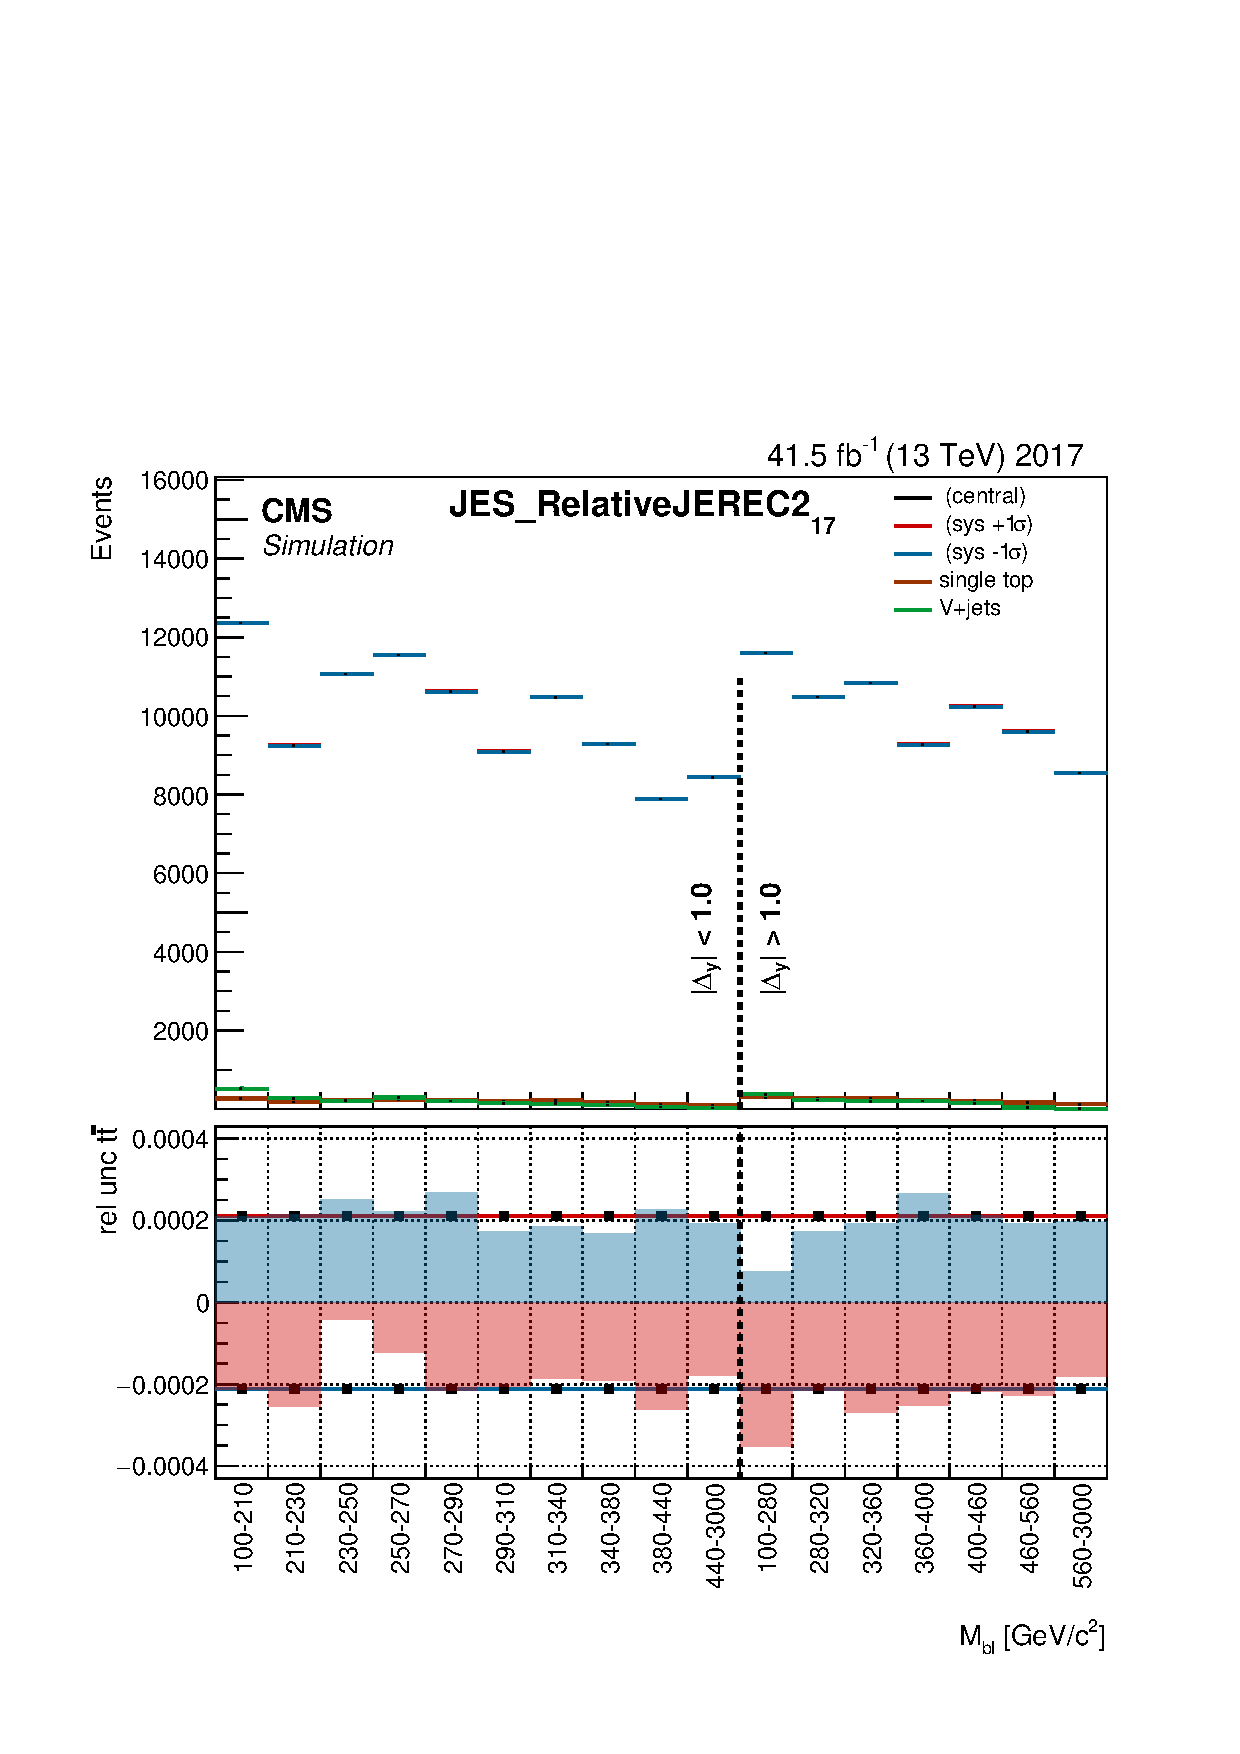
\includegraphics[width=.35\linewidth]{templates/JES_RelativeJEREC2_17}\hskip-.5cm
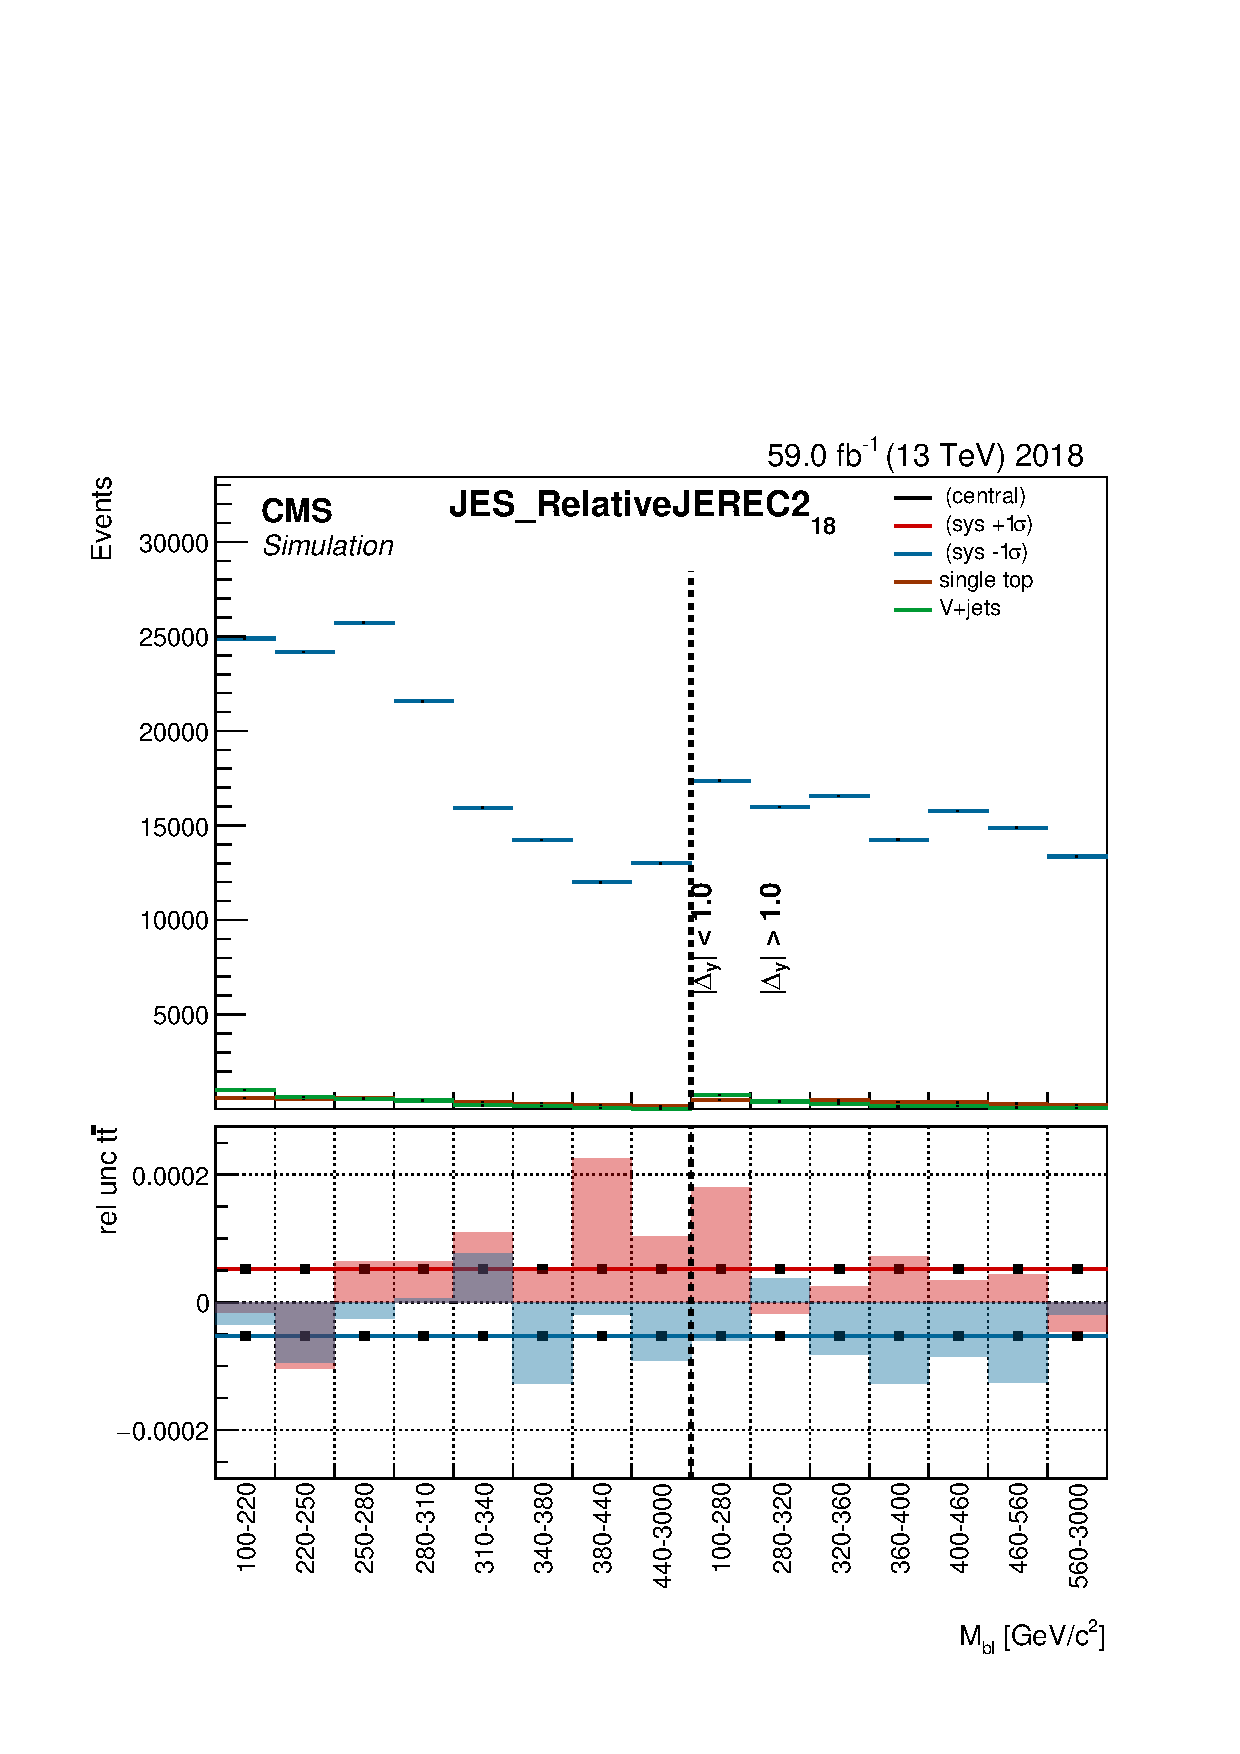
\includegraphics[width=.35\linewidth]{templates/JES_RelativeJEREC2_18}
\caption{JES\_RelativeJEREC2 templates}
\label{fig:JES-RelativeJEREC2_template}
\end{figure}

\begin{figure} \centering
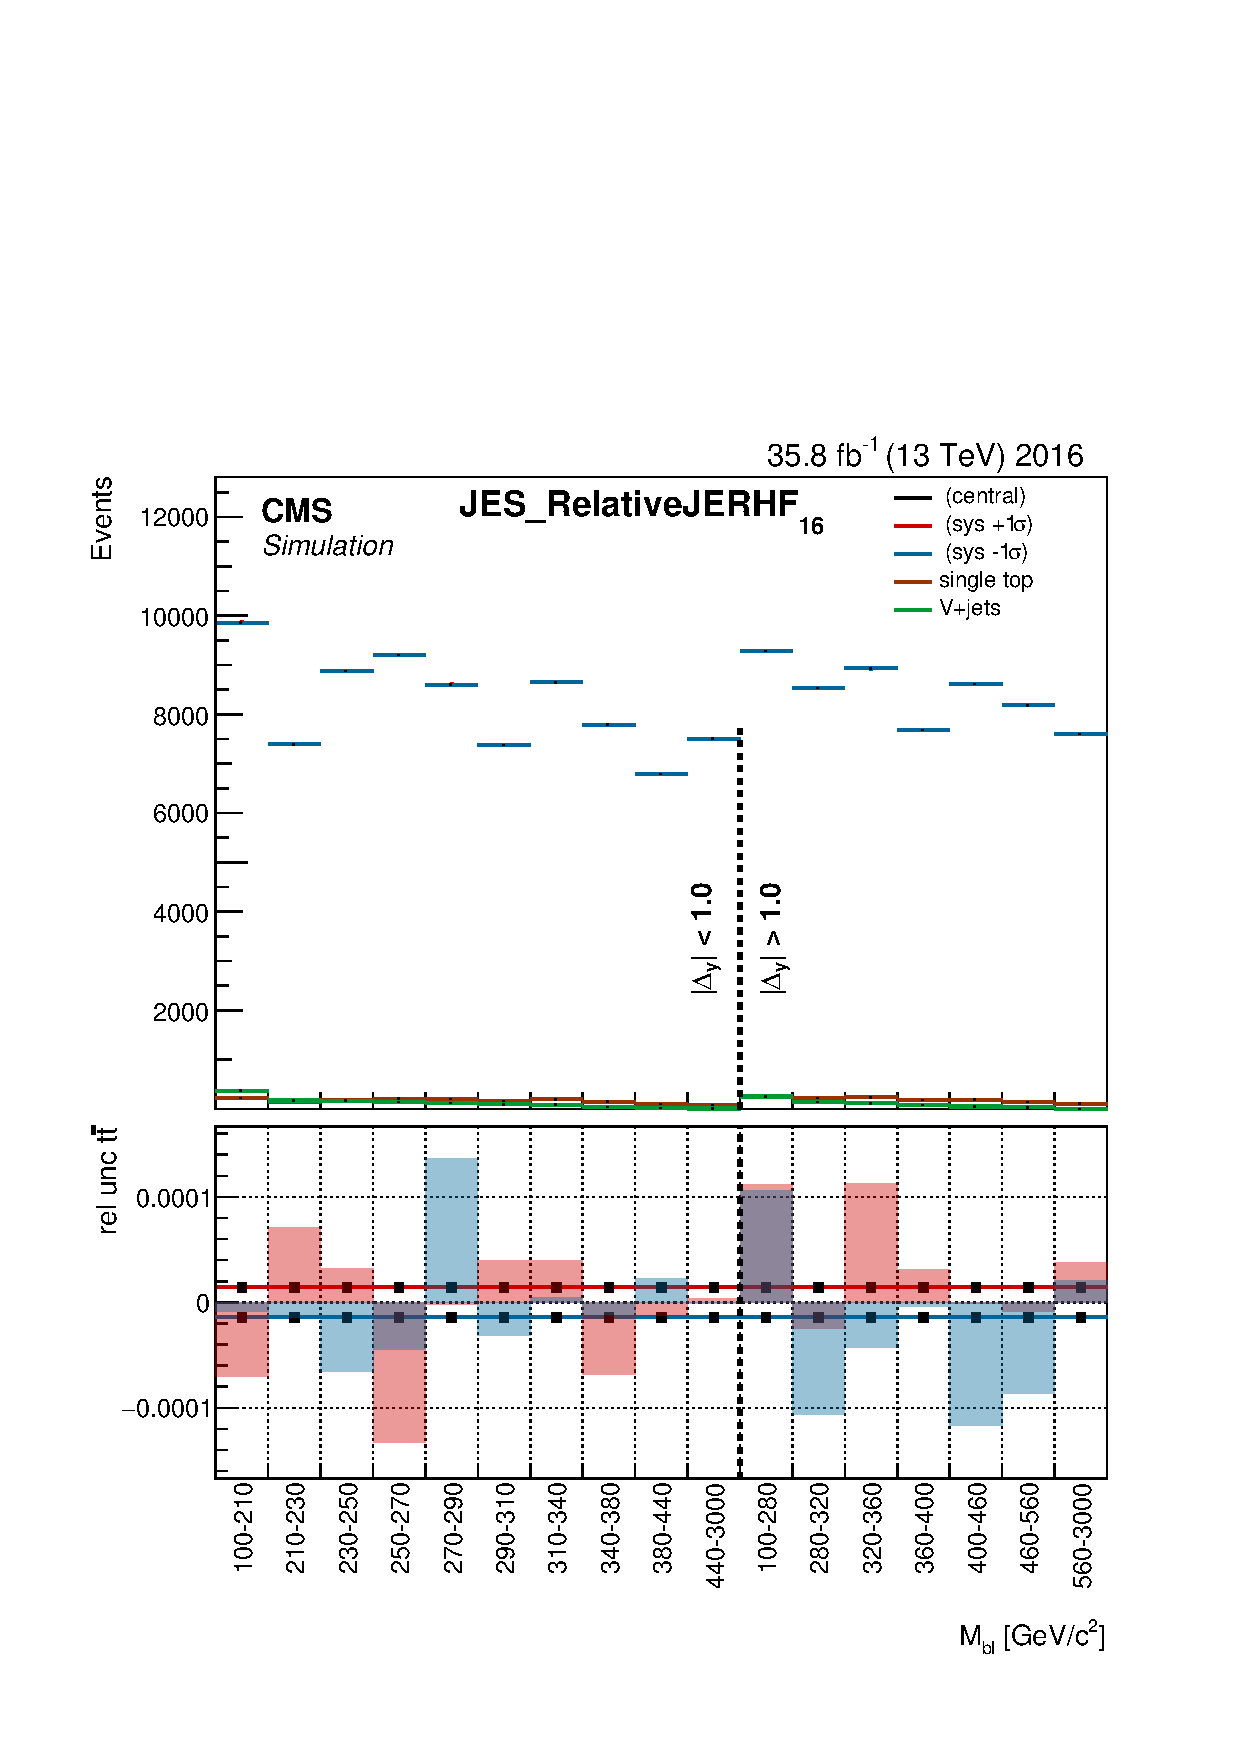
\includegraphics[width=.35\linewidth]{templates/JES_RelativeJERHF_16}\hskip-.5cm
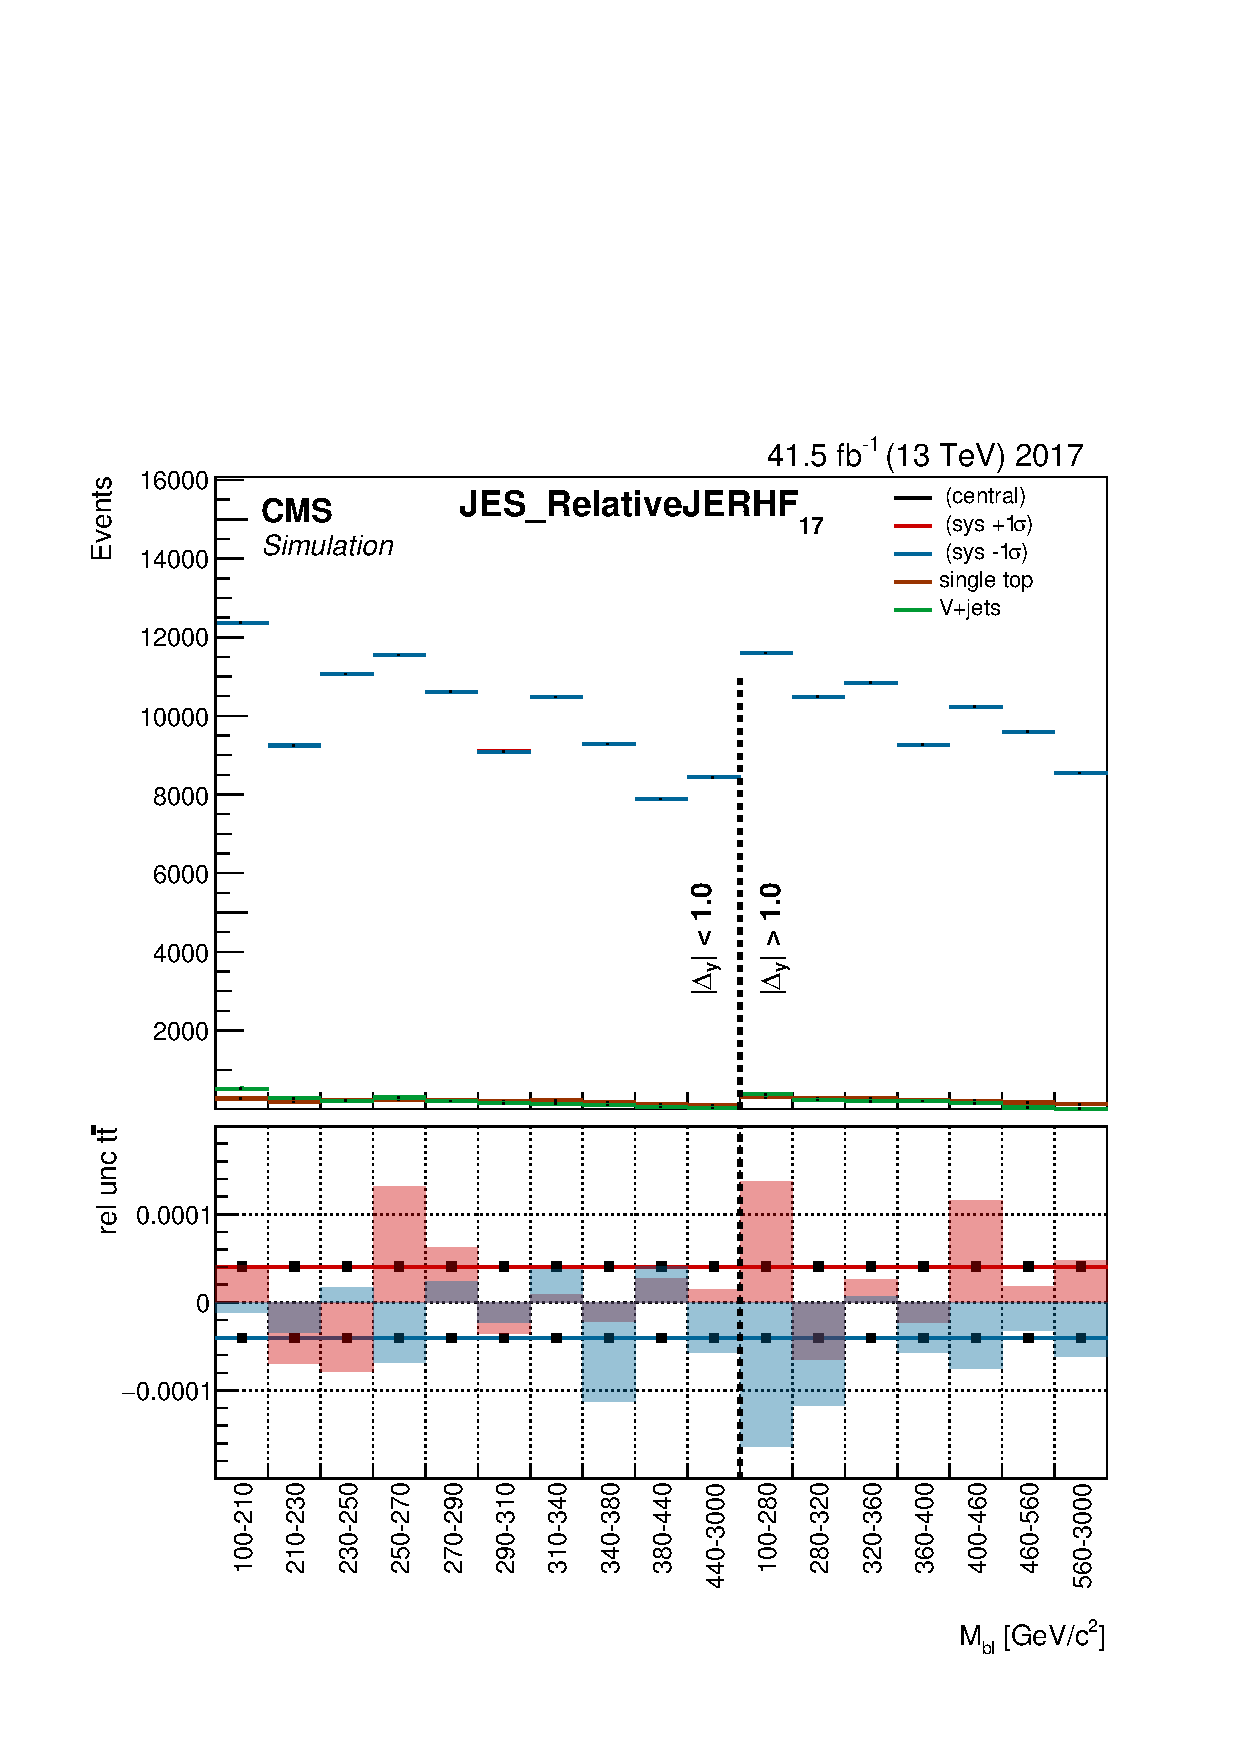
\includegraphics[width=.35\linewidth]{templates/JES_RelativeJERHF_17}\hskip-.5cm
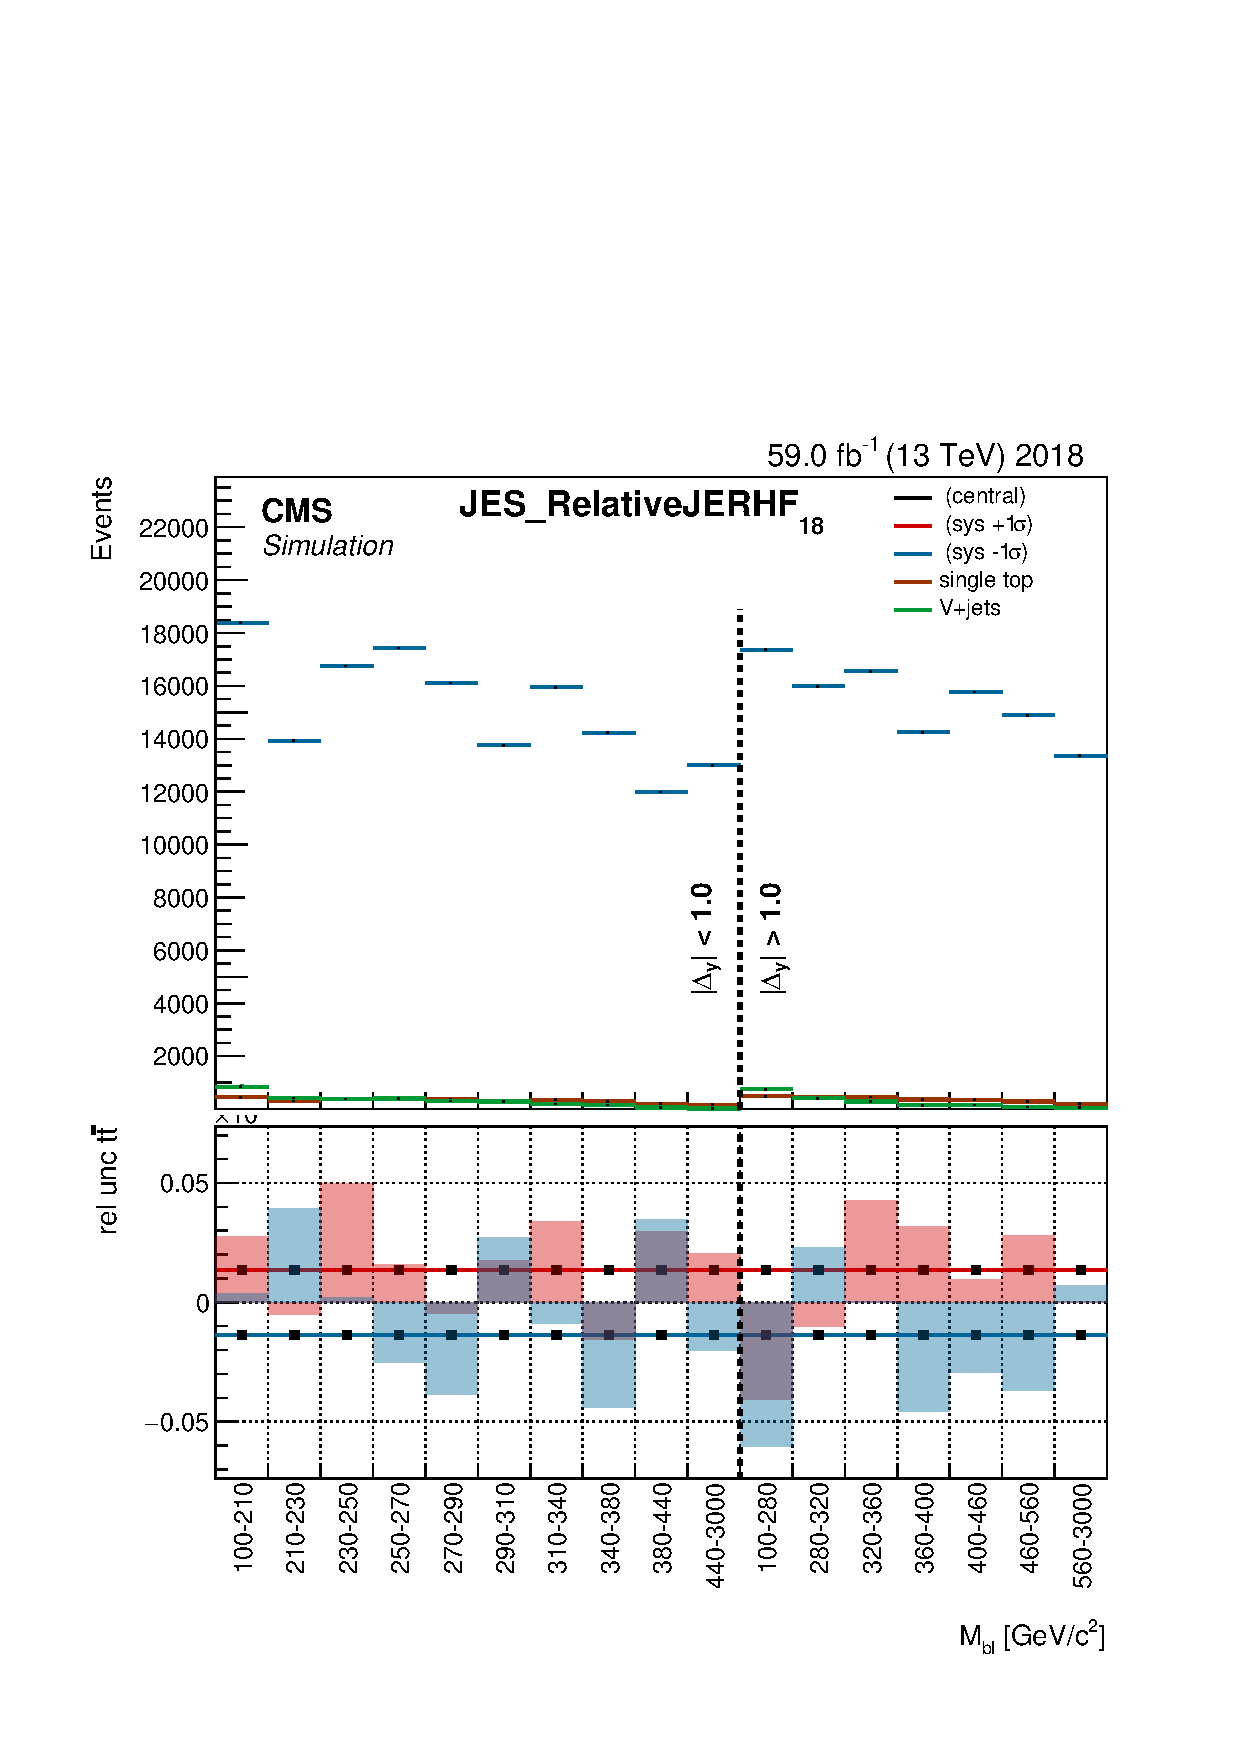
\includegraphics[width=.35\linewidth]{templates/JES_RelativeJERHF_18}
\caption{JES\_RelativeJERHF templates}
\label{fig:JES-RelativeJERHF_template}
\end{figure}

\begin{figure} \centering
\includegraphics[width=.35\linewidth]{templates/JES_RelativePtBB_16}\hskip-.5cm
\includegraphics[width=.35\linewidth]{templates/JES_RelativePtBB_17}\hskip-.5cm
\includegraphics[width=.35\linewidth]{templates/JES_RelativePtBB_18}
\caption{JES\_RelativePtBB templates}
\label{fig:JES-RelativePtBB_template}
\end{figure}

\begin{figure} \centering
\includegraphics[width=.35\linewidth]{templates/JES_RelativePtEC1_16}\hskip-.5cm
\includegraphics[width=.35\linewidth]{templates/JES_RelativePtEC1_17}\hskip-.5cm
\includegraphics[width=.35\linewidth]{templates/JES_RelativePtEC1_18}
\caption{JES\_RelativePtEC1 templates}
\label{fig:JES-RelativePtEC1_template}
\end{figure}

\begin{figure} \centering
\includegraphics[width=.35\linewidth]{templates/JES_RelativePtEC2_16}\hskip-.5cm
\includegraphics[width=.35\linewidth]{templates/JES_RelativePtEC2_17}\hskip-.5cm
\includegraphics[width=.35\linewidth]{templates/JES_RelativePtEC2_18}
\caption{JES\_RelativePtEC2 templates}
\label{fig:JES-RelativePtEC2_template}
\end{figure}

\begin{figure} \centering
\includegraphics[width=.35\linewidth]{templates/JES_RelativePtHF_16}\hskip-.5cm
\includegraphics[width=.35\linewidth]{templates/JES_RelativePtHF_17}\hskip-.5cm
\includegraphics[width=.35\linewidth]{templates/JES_RelativePtHF_18}
\caption{JES\_RelativePtHF templates}
\label{fig:JES-RelativePtHF_template}
\end{figure}

\begin{figure} \centering
\includegraphics[width=.35\linewidth]{templates/JES_RelativeSample_16}\hskip-.5cm
\includegraphics[width=.35\linewidth]{templates/JES_RelativeSample_17}\hskip-.5cm
\includegraphics[width=.35\linewidth]{templates/JES_RelativeSample_18}
\caption{JES\_RelativeSample templates}
\label{fig:JES-RelativeSample_template}
\end{figure}

\begin{figure} \centering
\includegraphics[width=.35\linewidth]{templates/JES_SinglePionECAL_16}\hskip-.5cm
\includegraphics[width=.35\linewidth]{templates/JES_SinglePionECAL_17}\hskip-.5cm
\includegraphics[width=.35\linewidth]{templates/JES_SinglePionECAL_18}
\caption{JES\_SinglePionECAL templates}
\label{fig:JES-SinglePionECAL_template}
\end{figure}

\begin{figure} \centering
\includegraphics[width=.35\linewidth]{templates/JES_SinglePionHCAL_16}\hskip-.5cm
\includegraphics[width=.35\linewidth]{templates/JES_SinglePionHCAL_17}\hskip-.5cm
\includegraphics[width=.35\linewidth]{templates/JES_SinglePionHCAL_18}
\caption{JES\_SinglePionHCAL templates}
\label{fig:JES-SinglePionHCAL_template}
\end{figure}

\begin{figure} \centering
\includegraphics[width=.35\linewidth]{templates/JES_TimePtEta_16}\hskip-.5cm
\includegraphics[width=.35\linewidth]{templates/JES_TimePtEta_17}\hskip-.5cm
\includegraphics[width=.35\linewidth]{templates/JES_TimePtEta_18}
\caption{JES\_TimePtEta templates}
\label{fig:JES-TimePtEta_template}
\end{figure}

\begin{figure} \centering
\includegraphics[width=.35\linewidth]{templates/JER_16}\hskip-.5cm
\includegraphics[width=.35\linewidth]{templates/JER_17}\hskip-.5cm
\includegraphics[width=.35\linewidth]{templates/JER_18}
\caption{JER templates}
\label{fig:JER_template}
\end{figure}


\begin{figure} \centering
\includegraphics[width=.35\linewidth]{templates/bdec_16}\hskip-.5cm
\includegraphics[width=.35\linewidth]{templates/bdec_17}\hskip-.5cm
\includegraphics[width=.35\linewidth]{templates/bdec_18}
\caption{bdec templates}
\label{fig:bdec_template}
\end{figure}

\begin{figure} \centering
\includegraphics[width=.35\linewidth]{templates/bfrag_16}\hskip-.5cm
\includegraphics[width=.35\linewidth]{templates/bfrag_17}\hskip-.5cm
\includegraphics[width=.35\linewidth]{templates/bfrag_18}
\caption{bfrag templates}
\label{fig:bfrag_template}
\end{figure}

\begin{figure} \centering
\includegraphics[width=.35\linewidth]{templates/btag_16}\hskip-.5cm
\includegraphics[width=.35\linewidth]{templates/btag_17}\hskip-.5cm
\includegraphics[width=.35\linewidth]{templates/btag_18}
\caption{btag templates}
\label{fig:btag_template}
\end{figure}

\begin{figure} \centering
\includegraphics[width=.35\linewidth]{templates/elrec_16}\hskip-.5cm
\includegraphics[width=.35\linewidth]{templates/elrec_17}\hskip-.5cm
\includegraphics[width=.35\linewidth]{templates/elrec_18}
\caption{elrec templates}
\label{fig:elrec_template}
\end{figure}

\begin{figure} \centering
\includegraphics[width=.35\linewidth]{templates/eltrg_16}\hskip-.5cm
\includegraphics[width=.35\linewidth]{templates/eltrg_17}\hskip-.5cm
\includegraphics[width=.35\linewidth]{templates/eltrg_18}
\caption{eltrg templates}
\label{fig:eltrg_template}
\end{figure}

% \begin{figure} \centering
% \includegraphics[width=.35\linewidth]{templates/flatsys18_16}\hskip-.5cm
% \includegraphics[width=.35\linewidth]{templates/flatsys18_17}\hskip-.5cm
% \includegraphics[width=.35\linewidth]{templates/flatsys18_18}
% \caption{flatsys18 templates}
% \label{fig:flatsys18_template}
% \end{figure}

\begin{figure} \centering
\includegraphics[width=.35\linewidth]{templates/fs_16}\hskip-.5cm
\includegraphics[width=.35\linewidth]{templates/fs_17}\hskip-.5cm
\includegraphics[width=.35\linewidth]{templates/fs_18}
\caption{fs templates}
\label{fig:fs_template}
\end{figure}

\begin{figure} \centering
\includegraphics[width=.35\linewidth]{templates/fsr_16}\hskip-.5cm
\includegraphics[width=.35\linewidth]{templates/fsr_17}\hskip-.5cm
\includegraphics[width=.35\linewidth]{templates/fsr_18}
\caption{fsr templates}
\label{fig:fsr_template}
\end{figure}

\begin{figure} \centering
\includegraphics[width=.35\linewidth]{templates/hd_16}\hskip-.5cm
\includegraphics[width=.35\linewidth]{templates/hd_17}\hskip-.5cm
\includegraphics[width=.35\linewidth]{templates/hd_18}
\caption{hd templates}
\label{fig:hd_template}
\end{figure}

\begin{figure} \centering
\includegraphics[width=.35\linewidth]{templates/isr_16}\hskip-.5cm
\includegraphics[width=.35\linewidth]{templates/isr_17}\hskip-.5cm
\includegraphics[width=.35\linewidth]{templates/isr_18}
\caption{isr templates}
\label{fig:isr_template}
\end{figure}

\begin{figure} \centering
\includegraphics[width=.35\linewidth]{templates/ltag_16}\hskip-.5cm
\includegraphics[width=.35\linewidth]{templates/ltag_17}\hskip-.5cm
\includegraphics[width=.35\linewidth]{templates/ltag_18}
\caption{ltag templates}
\label{fig:ltag_template}
\end{figure}




\begin{figure} \centering
\includegraphics[width=.32\linewidth]{templates/mtop_16_old}
\includegraphics[width=.32\linewidth]{templates/mtop_17_old}
\includegraphics[width=.32\linewidth]{templates/mtop_18_old}
\caption{mtop original templates. One can see common features, but the templates are too noisy for the smoothing to yield a reasonable shape. These are NOT included in the fit}
\label{fig:mtop_template_old}
\end{figure}

\begin{figure} \centering
\includegraphics[width=.32\linewidth]{templates/mtop_16}
\includegraphics[width=.32\linewidth]{templates/mtop_17}
\includegraphics[width=.32\linewidth]{templates/mtop_18}
\caption{mtop templates after combining all 3 years to make a single template. After combining and smoothing, we see a reasonable shape effect which captures the features shared between the 3 templates in Fig. \ref{fig:mtop_template_old}. Thus, one shape is used for all 3 years.}

\label{fig:mtop_template}
\end{figure}

\begin{figure} \centering
\includegraphics[width=.35\linewidth]{templates/murec_16}\hskip-.5cm
\includegraphics[width=.35\linewidth]{templates/murec_17}\hskip-.5cm
\includegraphics[width=.35\linewidth]{templates/murec_18}
\caption{murec templates}
\label{fig:murec_template}
\end{figure}

\begin{figure} \centering
\includegraphics[width=.35\linewidth]{templates/mutrg_16}\hskip-.5cm
\includegraphics[width=.35\linewidth]{templates/mutrg_17}\hskip-.5cm
\includegraphics[width=.35\linewidth]{templates/mutrg_18}
\caption{mutrg templates}
\label{fig:mutrg_template}
\end{figure}

\begin{figure} \centering
\includegraphics[width=.35\linewidth]{templates/prefire_16}\hskip-.5cm
\includegraphics[width=.35\linewidth]{templates/prefire_17}\hskip-.5cm
\caption{prefire templates}
\label{fig:pprefire_template}
\end{figure}

\begin{figure} \centering
\includegraphics[width=.35\linewidth]{templates/pdf0_16}\hskip-.5cm
\includegraphics[width=.35\linewidth]{templates/pdf0_17}\hskip-.5cm
\includegraphics[width=.35\linewidth]{templates/pdf0_18}
\caption{pdf0 templates}
\label{fig:pdf0_template}
\end{figure}

\begin{figure} \centering
\includegraphics[width=.35\linewidth]{templates/pdf1_16}\hskip-.5cm
\includegraphics[width=.35\linewidth]{templates/pdf1_17}\hskip-.5cm
\includegraphics[width=.35\linewidth]{templates/pdf1_18}
\caption{pdf1 templates}
\label{fig:pdf1_template}
\end{figure}

\begin{figure} \centering
\includegraphics[width=.35\linewidth]{templates/pdf2_16}\hskip-.5cm
\includegraphics[width=.35\linewidth]{templates/pdf2_17}\hskip-.5cm
\includegraphics[width=.35\linewidth]{templates/pdf2_18}
\caption{pdf2 templates}
\label{fig:pdf2_template}
\end{figure}

\begin{figure} \centering
\includegraphics[width=.35\linewidth]{templates/pdf3_16}\hskip-.5cm
\includegraphics[width=.35\linewidth]{templates/pdf3_17}\hskip-.5cm
\includegraphics[width=.35\linewidth]{templates/pdf3_18}
\caption{pdf3 templates}
\label{fig:pdf3_template}
\end{figure}

\begin{figure} \centering
\includegraphics[width=.35\linewidth]{templates/pdf4_16}\hskip-.5cm
\includegraphics[width=.35\linewidth]{templates/pdf4_17}\hskip-.5cm
\includegraphics[width=.35\linewidth]{templates/pdf4_18}
\caption{pdf4 templates}
\label{fig:pdf4_template}
\end{figure}

\begin{figure} \centering
\includegraphics[width=.35\linewidth]{templates/pdf5_16}\hskip-.5cm
\includegraphics[width=.35\linewidth]{templates/pdf5_17}\hskip-.5cm
\includegraphics[width=.35\linewidth]{templates/pdf5_18}
\caption{pdf5 templates}
\label{fig:pdf5_template}
\end{figure}

\begin{figure} \centering
\includegraphics[width=.35\linewidth]{templates/pdf6_16}\hskip-.5cm
\includegraphics[width=.35\linewidth]{templates/pdf6_17}\hskip-.5cm
\includegraphics[width=.35\linewidth]{templates/pdf6_18}
\caption{pdf6 templates}
\label{fig:pdf6_template}
\end{figure}

\begin{figure} \centering
\includegraphics[width=.35\linewidth]{templates/pdf7_16}\hskip-.5cm
\includegraphics[width=.35\linewidth]{templates/pdf7_17}\hskip-.5cm
\includegraphics[width=.35\linewidth]{templates/pdf7_18}
\caption{pdf7 templates}
\label{fig:pdf7_template}
\end{figure}

\begin{figure} \centering
\includegraphics[width=.35\linewidth]{templates/pdf8_16}\hskip-.5cm
\includegraphics[width=.35\linewidth]{templates/pdf8_17}\hskip-.5cm
\includegraphics[width=.35\linewidth]{templates/pdf8_18}
\caption{pdf8 templates}
\label{fig:pdf8_template}
\end{figure}

\begin{figure} \centering
\includegraphics[width=.35\linewidth]{templates/pdf9_16}\hskip-.5cm
\includegraphics[width=.35\linewidth]{templates/pdf9_17}\hskip-.5cm
\includegraphics[width=.35\linewidth]{templates/pdf9_18}
\caption{pdf9 templates}
\label{fig:pdf9_template}
\end{figure}


\begin{figure} \centering
\includegraphics[width=.35\linewidth]{templates/pdf_as_16}\hskip-.5cm
\includegraphics[width=.35\linewidth]{templates/pdf_as_17}\hskip-.5cm
\includegraphics[width=.35\linewidth]{templates/pdf_as_18}
\caption{pdf-as template }
\label{fig:pdfas_template}
\end{figure}


\clearpage



\begin{figure} \centering
\includegraphics[width=.35\linewidth]{templates/pu_16}\hskip-.5cm
\includegraphics[width=.35\linewidth]{templates/pu_17}\hskip-.5cm
\includegraphics[width=.35\linewidth]{templates/pu_18}
\caption{pu templates}
\label{fig:pu_template}
\end{figure}

\begin{figure} \centering
\includegraphics[width=.35\linewidth]{templates/rs_16}\hskip-.5cm
\includegraphics[width=.35\linewidth]{templates/rs_17}\hskip-.5cm
\includegraphics[width=.35\linewidth]{templates/rs_18}
\caption{rs templates}
\label{fig:rs_template}
\end{figure}

\begin{figure} \centering
\includegraphics[width=.35\linewidth]{templates/rsfs_16}\hskip-.5cm
\includegraphics[width=.35\linewidth]{templates/rsfs_17}\hskip-.5cm
\includegraphics[width=.35\linewidth]{templates/rsfs_18}
\caption{rsfs templates}
\label{fig:rsfs_template}
\end{figure}





\begin{figure} \centering
\includegraphics[width=.35\linewidth]{templates/tune_16}\hskip-.5cm
\includegraphics[width=.35\linewidth]{templates/tune_17}\hskip-.5cm
\includegraphics[width=.35\linewidth]{templates/tune_18}
\caption{tune templates}
\label{fig:tune_template}
\end{figure}



\clearpage

\bibliography{auto_generated}


